\documentclass[11pt,a4paper]{article}

% --------------------------------------------------
% Encoding and typography
% --------------------------------------------------
\usepackage[T1]{fontenc}
\usepackage[utf8]{inputenc}
% \usepackage{tgschola}
% \usepackage{libertinus}
%\usepackage{tgtermes}
\usepackage{tgpagella}
\usepackage[T1]{fontenc}
\usepackage{lmodern}
\usepackage{microtype}
\usepackage{tikz}
\usetikzlibrary{shapes.geometric, arrows.meta, positioning}

% --------------------------------------------------
% Page layout
% --------------------------------------------------
\usepackage[
a4paper,
margin=2.5cm
]{geometry}

\usepackage{setspace}
\setstretch{1.15}

\usepackage{float}

% --------------------------------------------------
% Mathematics and scientific notation
% --------------------------------------------------
\usepackage{amsmath}
\usepackage{amssymb}
\usepackage{siunitx}

% --------------------------------------------------
% Figures and tables
% --------------------------------------------------
\usepackage{graphicx}
\usepackage{booktabs}
\usepackage{caption}
\usepackage{subcaption}
\usepackage{tabularx}
\usepackage{etoolbox}

\graphicspath{{figures/}}

% --------------------------------------------------
% Colors and hyperlinks
% --------------------------------------------------
\usepackage{xcolor}

\definecolor{geosoilgreen}{HTML}{285943}

\usepackage[
colorlinks=true,
linkcolor=geosoilgreen,
citecolor=geosoilgreen,
urlcolor=blue
]{hyperref}

\usepackage{cleveref}

% Figure and table captions
\captionsetup{
	font={sf,small},
	labelfont={bf},
	justification=centering
}

% Table contents
\AtBeginEnvironment{tabular}{\sffamily\small}

% --------------------------------------------------
% Bibliography
% --------------------------------------------------
\usepackage[
backend=biber,
style=authoryear,
sorting=nyt
]{biblatex}

\addbibresource{references.bib}


\DeclareFieldFormat{labelname}{\mkbibbrackets{#1}}
\DeclareFieldFormat{labeldate}{\mkbibbrackets{#1}}



% --------------------------------------------------
% Document metadata
% --------------------------------------------------
\title{
	\textbf{GeoSoil-Cuba}\\[0.3cm]
	\large
	Integrating Soil Mapping, Land Cover, and
	Sentinel-2 Imagery for Geospatial Analysis in Cuba
}

\author{Ben Tamayo}

\date{October 2026}

% --------------------------------------------------
% Document
% --------------------------------------------------
\begin{document}
	
	\maketitle
	
	% --------------------------------------------------
	% Abstract
	% --------------------------------------------------
\begin{abstract}
	
	GeoSoil-Cuba is an open-source geospatial analysis project
	that integrates soil mapping, land-cover information, and
	Sentinel-2 satellite imagery within a reproducible
	Python-based workflow. The study focuses on Jaruco,
	Mayabeque Province, Cuba, and combines soil-map preparation
	and spatial validation with satellite-derived vegetation
	monitoring. A 1:25,000-scale soil dataset was evaluated
	within an Area of Interest (AOI) covering approximately
	178.47~km$^2$. Soil polygons covered 162.85~km$^2$
	(91.25\% of the AOI), while 4.20~km$^2$ (2.35\%) remained
	uncovered outside the mapped water-related gaps. Topological
	assessment identified 90 pairs of soil polygons with
	positive-area overlaps, highlighting issues requiring
	further validation. For vegetation monitoring, Sentinel-2
	Level-2A imagery acquired between November 2025 and June
	2026 was processed to calculate the Normalized Difference
	Vegetation Index (NDVI). Fifteen acquisitions met a
	regional cloud-coverage criterion of less than 10\% within
	a unified agricultural region of approximately 16.22~km$^2$.
	Mean NDVI declined from 0.688 in November 2025 to 0.466
	in March 2026, before increasing to 0.737 in June 2026.
	A complementary analysis examined NDVI variability in
	three locally verified potato fields using circular
	sampling polygons digitized in QGIS. The results
	demonstrate the utility of integrating historical soil
	information, land-cover data, and satellite observations
	in a documented geospatial workflow. However, the observed
	vegetation-index patterns do not establish causal
	relationships between soil properties, crop development,
	and agricultural management.
	
\end{abstract}
	
	\noindent
	\textbf{Keywords:}
	Geospatial Analysis;
	Soil Mapping;
	Remote Sensing;
	Sentinel-2;
	NDVI;
	Python;
	GIS.
	
	\vspace{0.5cm}
	
	% --------------------------------------------------
	% Main sections
	% --------------------------------------------------
	
\section{Introduction}
\label{sec:introduction}

Soil characteristics and vegetation conditions are closely related
components of terrestrial ecosystems. Understanding their spatial
relationships is important for agricultural assessment, land-resource
management, and environmental monitoring. Geographic Information
Systems (GIS) and satellite remote sensing provide complementary
sources of information for investigating these relationships across
different spatial and temporal scales.

Conventional soil maps describe the spatial distribution of soil
types and associated characteristics. However, integrating these
datasets with contemporary geospatial information may require
coordinate reference system harmonization, geometry validation,
spatial clipping, attribute interpretation, and assessment of
mapping completeness. These operations are particularly relevant
when working with historical cartographic datasets that were
originally developed using formats and classification systems
different from those commonly employed in modern geospatial
workflows.

Satellite observations complement soil mapping by providing
repeated measurements of land-surface conditions. In particular,
the Sentinel-2 mission supplies multispectral imagery suitable
for vegetation monitoring. The Normalized Difference Vegetation
Index (NDVI), calculated from red and near-infrared reflectance,
provides an indirect indicator of vegetation greenness and canopy
development. Temporal NDVI observations can characterize changes
in vegetation conditions, although their interpretation depends
on land cover, acquisition quality, and agricultural context.

GeoSoil-Cuba is an open-source geospatial analysis project
developed to integrate soil mapping, land-cover information,
and Sentinel-2 satellite imagery within a reproducible
Python-based workflow. The project focuses on a study area
in Jaruco, Mayabeque Province, Cuba, using a 1:25,000-scale
soil map as the primary spatial framework for subsequent
soil--vegetation analysis.

The workflow has two complementary analytical components. The
first prepares and evaluates the soil dataset through geometry
validation and repair, coordinate reference system harmonization,
spatial intersection and clipping, classification interpretation,
and soil-map coverage assessment. Water-body information helps
distinguish areas excluded from terrestrial soil mapping from
unresolved gaps in the source dataset. The second component
processes Sentinel-2 observations to examine temporal NDVI
variability in a selected agricultural region and in three
locally verified potato-field samples. Together, these components
provide spatially organized datasets and exploratory vegetation
observations without presuming a causal relationship between
mapped soil classes and vegetation dynamics.

The main objectives of this study are to:

\begin{enumerate}
	
	\item Prepare and validate the existing soil cartographic
	information for geospatial analysis within the selected
	Area of Interest (AOI).
	
	\item Evaluate the spatial completeness and classification
	consistency of the soil dataset, distinguishing mapped
	water bodies from unresolved soil-data gaps.
	
	\item Integrate the processed soil information with
	land-cover classifications and organize it for analysis
	alongside Sentinel-2 observations.
	
	\item Process Sentinel-2 imagery and characterize temporal
	NDVI variability within a selected agricultural region.
	
	\item Compare NDVI observations from three locally verified
	potato-field samples, recognizing the limits of inferring
	crop development from satellite reflectance alone.
	
\end{enumerate}

The contribution of GeoSoil-Cuba lies primarily in the
integration, validation, and documentation of heterogeneous
geospatial datasets through an open-source analytical workflow.
Rather than proposing a new soil classification system or
establishing causal relationships between soil properties and
vegetation performance, the project provides a documented
framework for exploratory soil--vegetation analysis that can
be extended through additional satellite observations,
field measurements, and spatial datasets.

	\section{Study Area}
\label{sec:study-area}

The GeoSoil-Cuba study area is located in Jaruco,
Mayabeque Province, western Cuba. The Area of Interest
(AOI) covers approximately
\SI{178.47}{\square\kilo\metre} and encompasses
agricultural landscapes, natural and semi-natural
vegetation, and the Mampostón reservoir (\Cref{fig:study_area_location}). Administrative boundaries were obtained from
the GADM database, version 4.1, using the
Cuba GeoPackage dataset
(\texttt{gadm41\_CUB.gpkg})
\parencite{gadm2022}. Both location maps were prepared in QGIS.
Cartographic elements, including coordinate
grids, scale bars, north arrows, and geographic
labels, were configured using the QGIS
print layout. 

This geographic setting provides a basis for integrating
historical soil cartography, land-cover information,
and satellite-derived vegetation observations.

\begin{figure}[htbp]
	\centering
	
	% (a) Geographic location of Mayabeque, Cuba
	\begin{subfigure}[t]{0.48\textwidth}
		\centering
		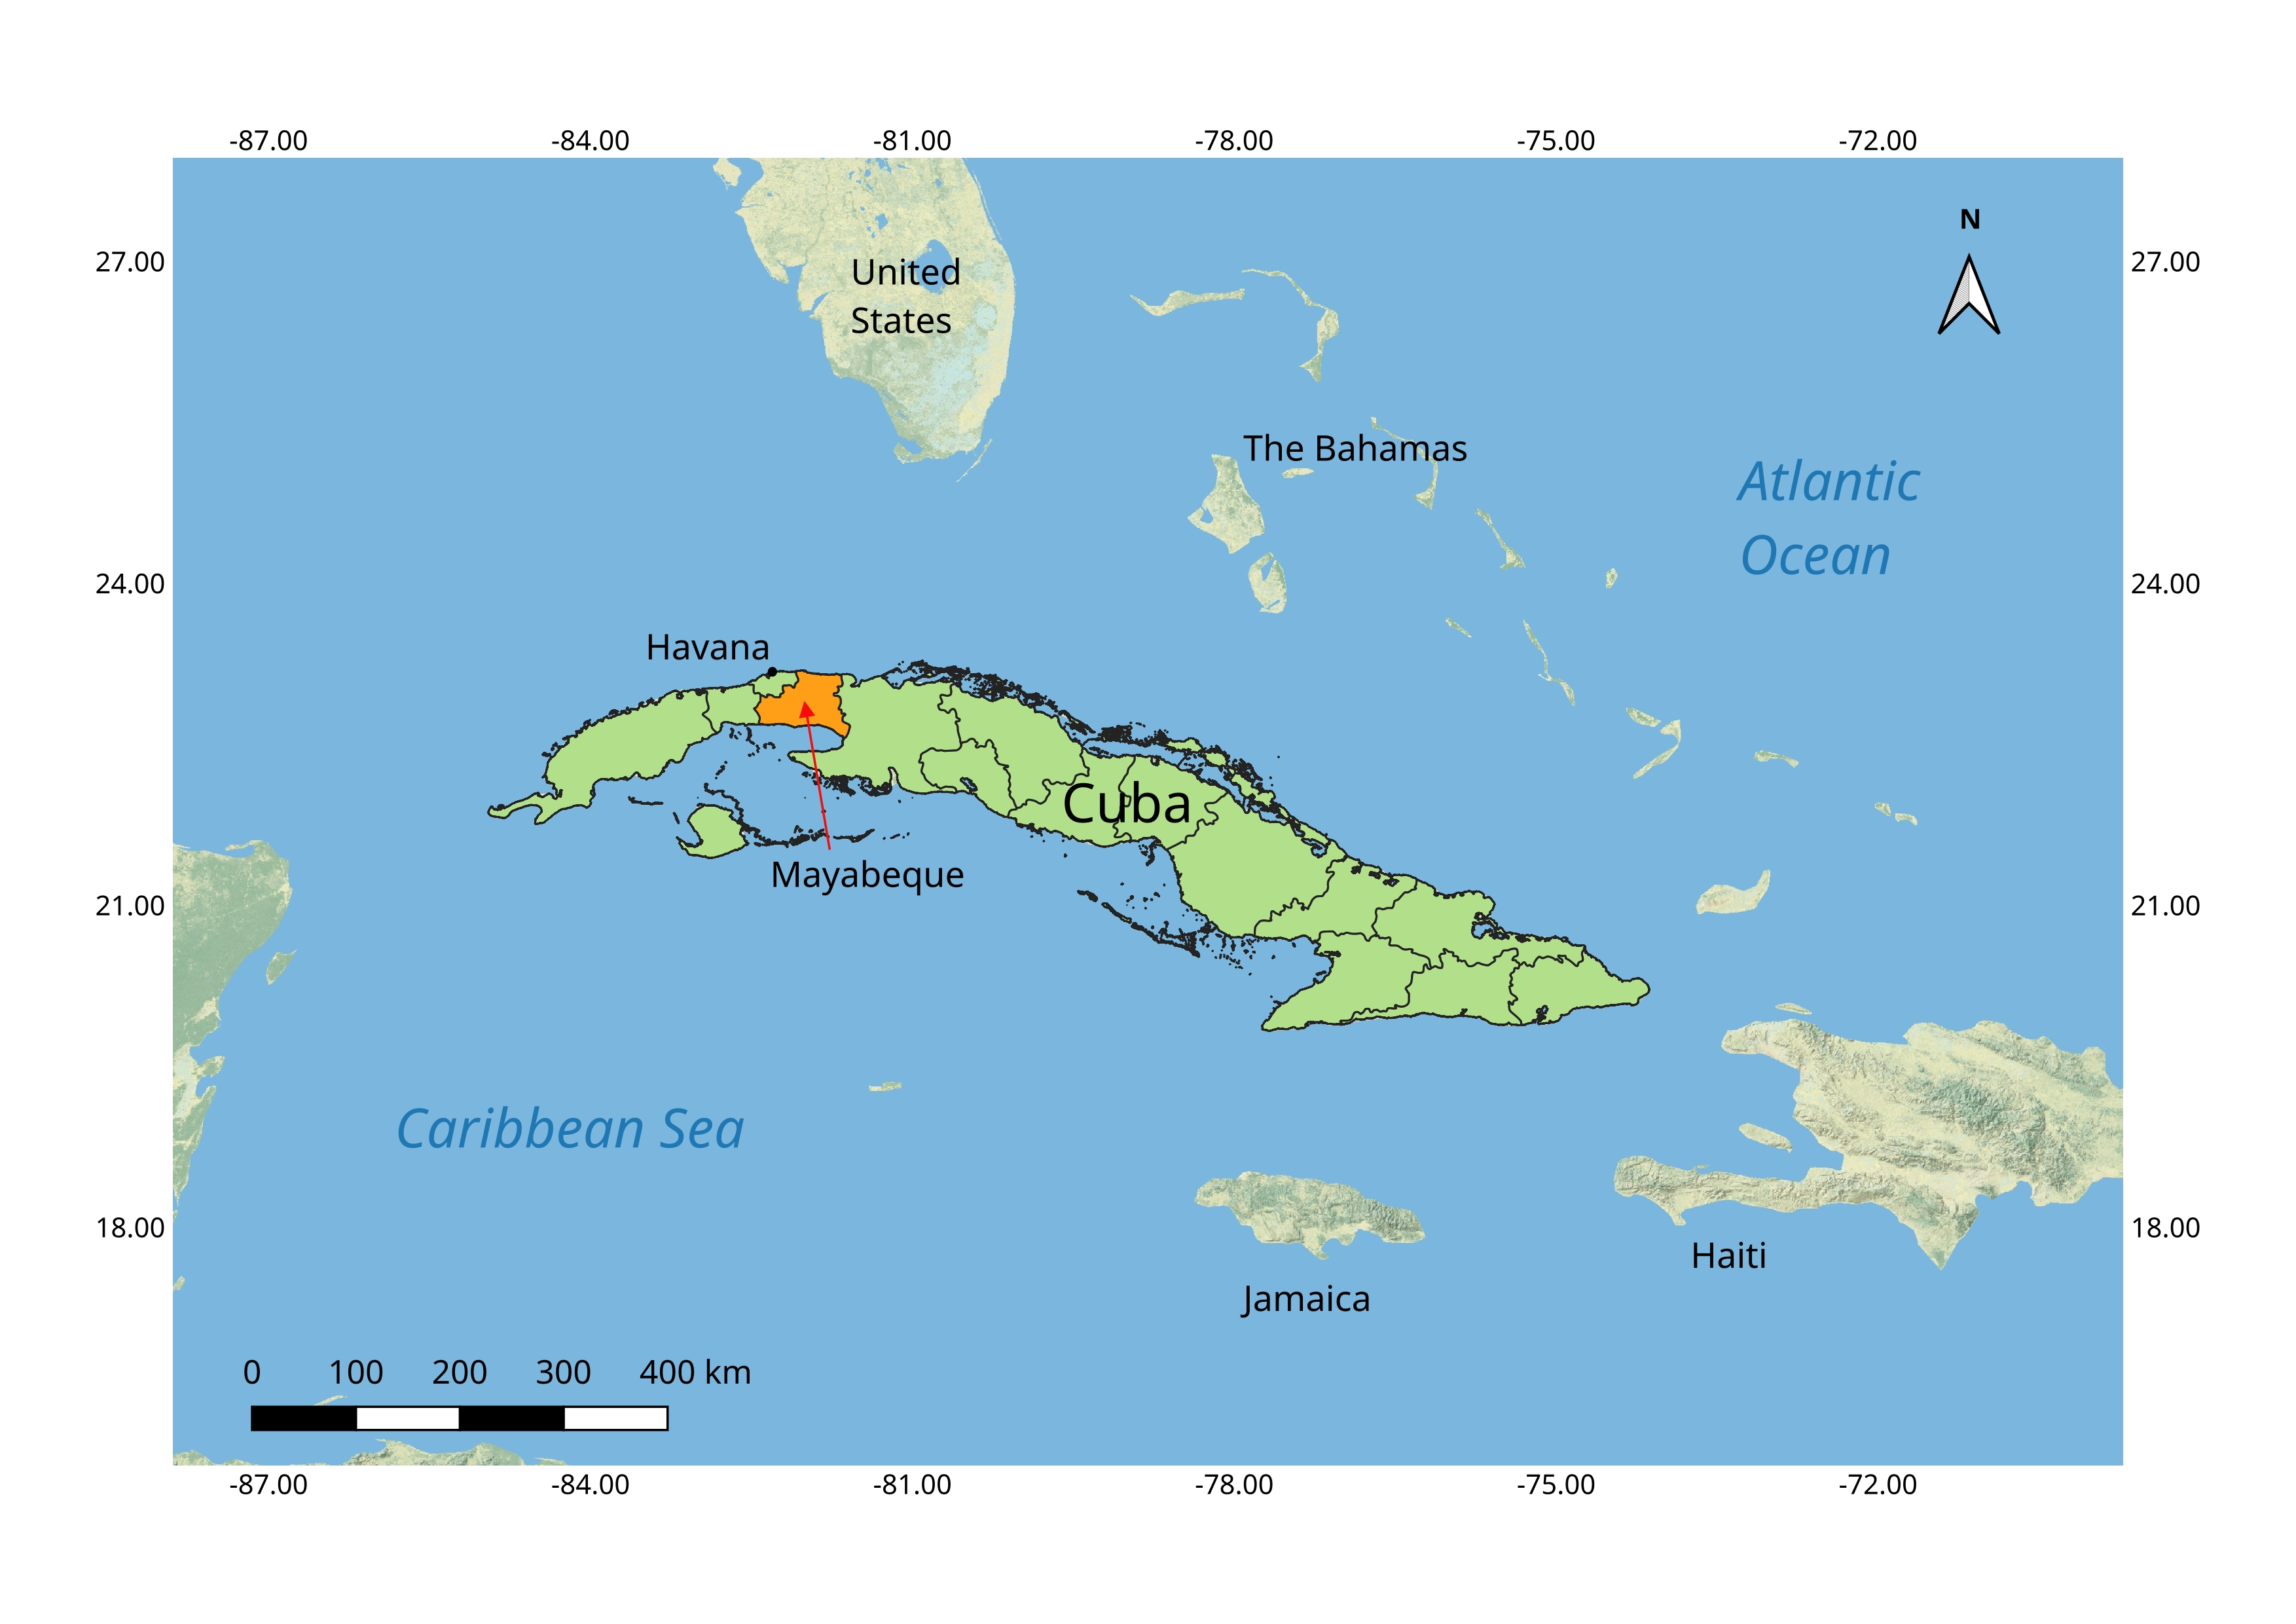
\includegraphics[
		width=\linewidth,
		height=5.5cm,
		keepaspectratio
		]{../figures/caribe-cuba.jpg}
		
		\caption{Geographic location of Mayabeque Province, Cuba.}
		\label{fig:mayabeque_location}
	\end{subfigure}
	\hfill
	% (b) Study area in Jaruco, Mayabeque
	\begin{subfigure}[t]{0.48\textwidth}
		\centering
		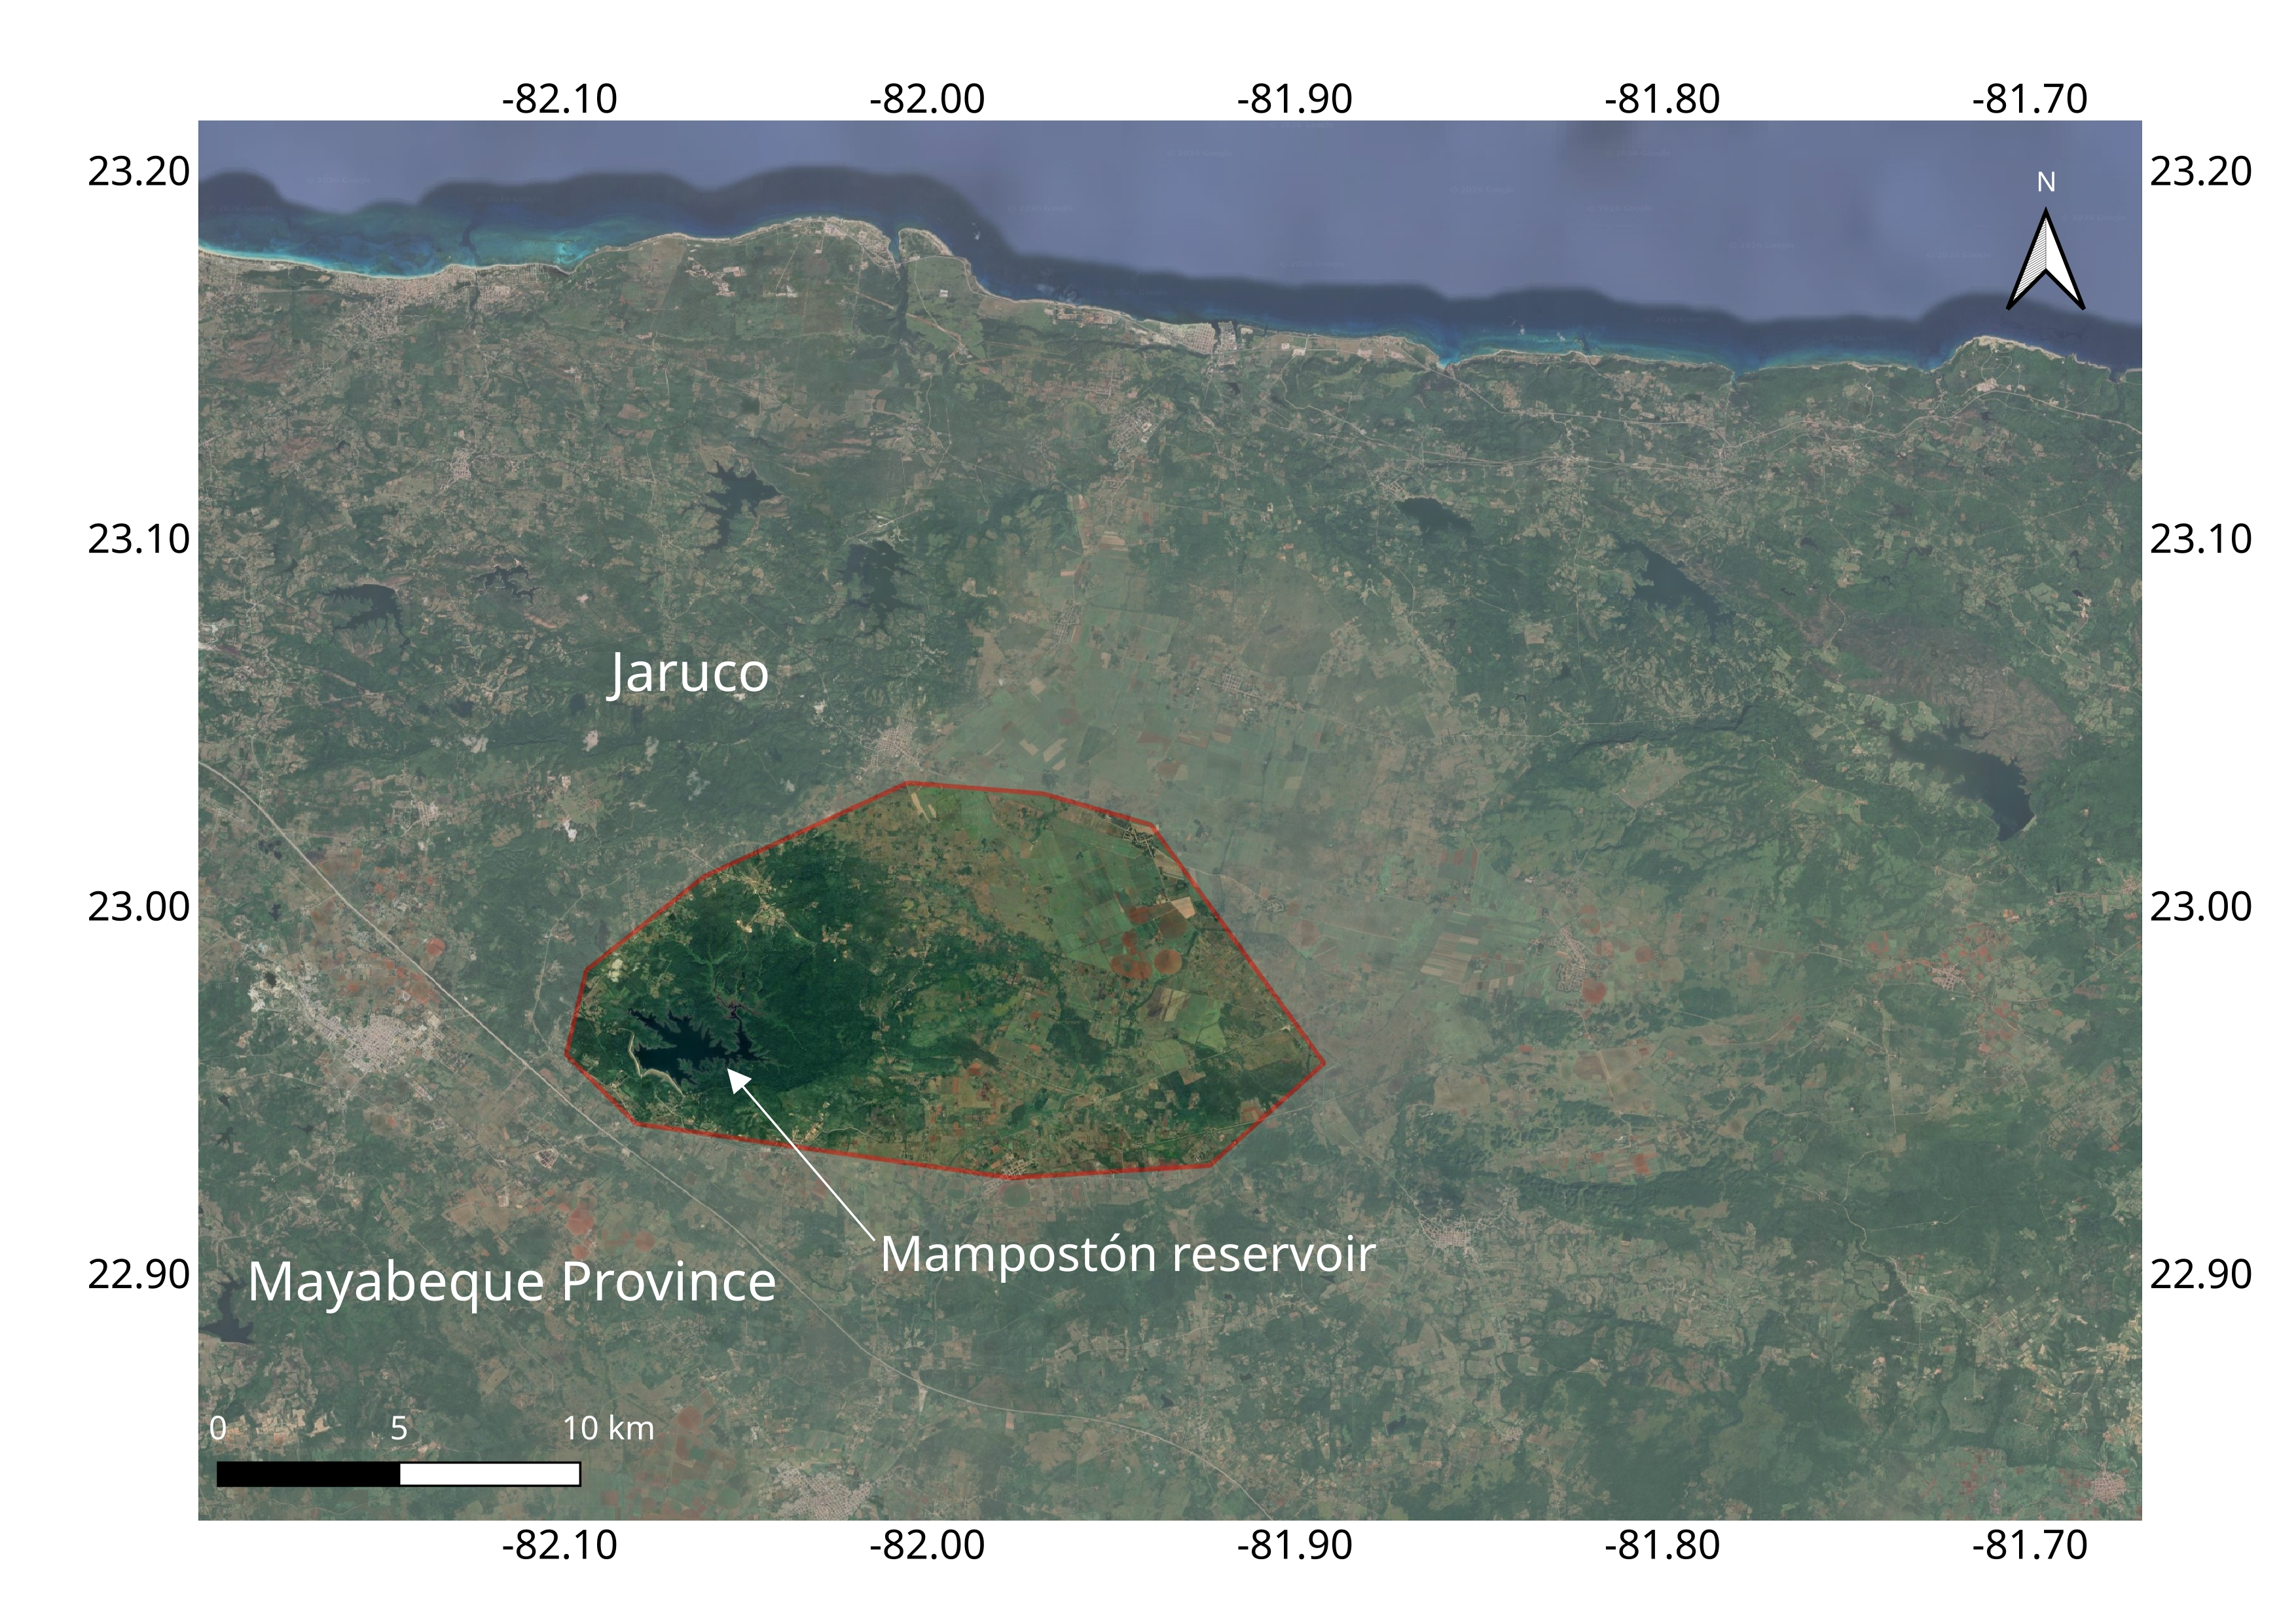
\includegraphics[
		width=\linewidth,
		height=5.5cm,
		keepaspectratio
		]{../figures/escala-mayabeque.jpg}
		
		\caption{Study area in Jaruco, Mayabeque Province.}
		\label{fig:jaruco_study_area}
	\end{subfigure}
	
	\caption{
		Geographic location of the study area:
		(a) Mayabeque Province within Cuba and
		(b) study area in Jaruco Municipality,
		Mayabeque Province.
		Maps prepared by the author using QGIS.
		Administrative boundaries derived from
		GADM version 4.1~\parencite{gadm2022}.
	}
	\label{fig:study_area_location}
\end{figure}

The AOI was defined using a geographic boundary
provided in Keyhole Markup Language (KML) format.
The original boundary uses the WGS 84 geographic
coordinate reference system (EPSG:4326). Its
approximate geographic extent ranges from
\ang{22.92585} to \ang{23.03332} north latitude
and from \ang{-82.09837} to \ang{-81.89215}
longitude.

For spatial analyses involving the historical soil
map, the AOI was transformed to NAD27 / Cuba Norte
(EPSG:3795), the projected coordinate reference
system used by the source cartographic dataset.
This transformation facilitates spatial
intersection, clipping, and area calculations
within a common coordinate reference system.

The Mampostón reservoir is a relevant geographic
feature within the AOI. Because open-water surfaces
are not expected to be represented by terrestrial
soil mapping units, their presence must be
considered when assessing soil-map coverage.
Accordingly, areas without mapped soil information
must be distinguished from water surfaces and
from other gaps that may remain within the
terrestrial analysis area.

Within the broader AOI, a unified agricultural
region was delineated for the regional NDVI
time-series analysis. A complementary analysis
examined vegetation-index observations within
three locally verified potato fields, represented
by sampling polygons digitized in QGIS. These
spatial units support different analytical
purposes: the AOI provides the overall context
for soil and land-cover integration, whereas the
agricultural region and field samples support
the examination of vegetation variability at
regional and field scales, respectively.

The study area was selected to evaluate the
integration and spatial consistency of existing
soil cartographic information, land-cover
classifications, and satellite observations.
The combined analyses provide a basis for
assessing soil-map coverage and examining
temporal vegetation-index patterns without
assuming that observed NDVI differences are
caused by soil properties or agricultural
management.


	\section{Data Sources and Technical Environment}
\label{sec:data-sources}

This study integrates existing soil and ancillary
spatial datasets with Sentinel-2 satellite imagery
to examine soil-map coverage, vegetation
distribution, and temporal vegetation dynamics
within the study area which were obtained
from the Sentinel-2 Level-2A product collection
through the Copernicus Data Space Ecosystem (CDSE) \mkbibbrackets{\cite{drusch2012sentinel2}}. The workflow combines
vector-data preparation and spatial analysis
with satellite image processing and NDVI-based
assessment.

The principal datasets, their spatial
characteristics, and their roles in the analysis
are summarized in
\Cref{tab:data-sources}.

\begin{table}[H]
	\centering
	\caption{Summary of spatial and satellite data
		sources used in the GeoSoil-Cuba workflow.}
	\label{tab:data-sources}
	\small
	\begin{tabularx}{\textwidth}{
			@{}
			p{2.6cm}
			p{2.5cm}
			p{2.8cm}
			X
			@{}
		}
		\toprule
		\textbf{Dataset} &
		\textbf{Source or format} &
		\textbf{Spatial reference} &
		\textbf{Role in the study} \\
		\midrule
		
		Soil map &
		Faculty of Geography, University of Havana;
		MapInfo TAB &
		NAD 27 Cuba datum; Lambert Conformal Conic;
		metres &
		Delineation and analysis of mapped soil units
		within the study area. Original scale:
		1:25,000. \\
		
		Area of Interest (AOI) &
		KML boundary &
		WGS 84 geographic coordinates
		(EPSG:4326) &
		Defines the study-area boundary and spatial
		extent of the analysis. \\
		
		Water bodies &
		Faculty of Geography, University of Havana;
		MapInfo TAB &
		As supplied; harmonized for spatial analysis &
		Identification of water surfaces and
		interpretation of apparent gaps in soil-map
		coverage. \\
		
		Vegetation and land cover &
		Faculty of Geography, University of Havana;
		vector dataset &
		As supplied; harmonized for spatial analysis &
		Integration of soil units with vegetation
		and land-cover attributes. \\
		
		Sentinel-2 imagery &
		Copernicus Data Space Ecosystem;
		Level-2A products &
		Tiles T17QLF and T17QMF;
		bands B04 and B08 at 10 m resolution;
		SCL at 20 m &
		Satellite-based vegetation analysis,
		including NDVI calculation and temporal
		assessment. Search period: November 2025
		to June 2026. \\
		
		\bottomrule
	\end{tabularx}
\end{table}


\subsection{Soil and Ancillary Spatial Data}
\label{subsec:soil-data}

The primary soil dataset consists of a
1:25,000-scale soil map of Mayabeque Province,
Cuba, distributed in MapInfo format. The dataset
contains polygon geometries representing mapped
soil units and associated attributes describing
soil types and subtypes according to the
classification system used in the source database.

The soil map uses the NAD27 / Cuba Norte
projected coordinate reference system
(EPSG:3795). Its original projection definition
was examined and standardized before spatial
processing.

The Area of Interest (AOI) was defined using a
polygon provided in Keyhole Markup Language
(KML) format, originally referenced to WGS 84
(EPSG:4326). The AOI was transformed to the
soil map's projected coordinate reference system
for the relevant spatial operations.

An additional water-body dataset, also supplied
in MapInfo format, was incorporated to identify
the Mampostón reservoir and distinguish mapped
water surfaces from areas lacking soil-map
coverage.

The original spatial datasets were preserved
unchanged. Derived geometries and attributes
were stored separately to maintain traceability
throughout the analytical workflow.

The original production dates and authorship
of the soil and ancillary datasets have not
been independently verified. Their spatial
and thematic interpretation must therefore
account for the characteristics and limitations
of the supplied source data.


\subsection{Vegetation and Land-Cover Data}
\label{subsec:land-cover-data}

Vegetation and land-cover information was obtained
from an existing vector dataset containing
categorical descriptions of vegetation and
land-cover units.

The dataset includes the attributes
\texttt{LCNAME}, \texttt{NEWVEG}, and
\texttt{TNC\_CLASS}, which provide complementary
classification information.

These attributes were examined and incorporated
into the spatial integration workflow to
characterize vegetation and land-cover
categories associated with the mapped soil units.

The vegetation dataset was processed independently
from the Sentinel-2 imagery. Its categorical
classifications therefore represent information
from an existing spatial dataset rather than
land-cover classes derived from the satellite
observations analyzed in this study.

The production date and original classification
methodology of the vegetation dataset have not
been independently verified. Consequently,
its temporal correspondence with the
2025--2026 satellite observations cannot be
assumed.

The soil, water-body, and vegetation-cover
datasets were provided courtesy of the Faculty
of Geography, University of Havana, Cuba
(Facultad de Geografía, Universidad de La Habana),
with permission for research, analysis, and
public redistribution. The institution is
acknowledged as the data provider; the original
production dates and authorship of these datasets
have not been independently verified.


\subsection{Sentinel-2 Satellite Imagery}
\label{subsec:sentinel-data}

Multispectral satellite observations were obtained
from the Sentinel-2 Level-2A product collection
through the Copernicus Data Space Ecosystem
(CDSE).

Satellite products were discovered using the
SpatioTemporal Asset Catalog (STAC) interface,
which supports searches based on geographic
extent, acquisition date, and product metadata.

The catalogue search covered the period from
November 2025 through June 2026. Products
associated with Sentinel-2 tiles T17QLF and
T17QMF were considered for the study area.

The analysis focused on the red (B04) and
near-infrared (B08) spectral bands, both provided
at a spatial resolution of 10 m. The Scene
Classification Layer (SCL), available at a
spatial resolution of 20 m, was used to support
quality screening and the assessment of
potential cloud and shadow contamination.

The initial satellite inventory contained
226 observations. Following image processing,
32 NDVI rasters were prepared for the selected
agricultural analysis region. A subsequent
regional cloud-screening procedure retained
15 acquisitions satisfying the criterion of
less than 10\% cloud coverage within that region.

This regional criterion reduced the influence
of cloud contamination but did not establish
that all pixels in the retained observations
were free of clouds, haze, or shadows.

Detailed acquisition selection, radiometric
correction, quality screening, and NDVI
calculation procedures are described in
\Cref{sec:methodology}.


\subsection{Software and Technical Environment}
\label{subsec:software}

GeoSoil-Cuba was developed using an open-source
Python geospatial environment managed through
Conda, with packages obtained primarily from
the \texttt{conda-forge} channel.

The documented environment uses Python 3.12.14
and GDAL 3.13.3.

Vector-data processing was performed using
GeoPandas 1.1.4 and Shapely 2.1.2, while
coordinate reference system transformations
were supported by PyProj 3.8.0.

Raster processing was supported by Rasterio
1.5.1, including the handling of georeferenced
satellite imagery and derived NDVI products.

NumPy 2.5.3 and Pandas 3.0.5 provided numerical
and tabular data processing capabilities,
respectively. Matplotlib 3.11.1 was used to
generate analytical figures and visualizations.

Sentinel-2 catalogue discovery was supported
by PySTAC Client 0.9.0, while Requests 2.34.2
provided HTTP communication functionality.

The analytical workflow was organized into
Jupyter notebooks, with JupyterLab 4.6.3
included in the documented environment.
QGIS 3.44.14-Solothurn was also used for the visual selection
and digitization of the three potato-field
sampling polygons.

The Conda environment specification and project
source code provide a record of the principal
software dependencies used in the analysis.
The software versions reported here correspond
to the documented environment and should be
verified against the final environment
specification before publication.


\subsection{Data Characteristics and Limitations}
\label{subsec:data-limitations}

The integration of historical soil cartography,
existing vegetation classifications, and
satellite observations introduces differences
in spatial representation, classification
structure, and temporal coverage.

The soil dataset represents mapped soil units
rather than direct measurements of contemporary
soil conditions. Its interpretation is therefore
constrained by the characteristics of the source
cartographic dataset, including its original
scale, soil classification system, and spatial
completeness. The dataset uses a Lambert
Conformal Conic projection referenced to the
NAD 27 Cuba datum, with coordinates expressed
in metres. The original map scale and
classification metadata should be considered
when interpreting the spatial detail and
thematic meaning of the mapped soil units.

The vegetation dataset provides categorical
land-cover information, whereas Sentinel-2
observations describe spectral conditions
at specific acquisition dates. Because the
original production date of the vegetation
dataset has not been verified, these sources
cannot be assumed to represent the same period.

Satellite-derived vegetation indices may also
be affected by atmospheric conditions, residual
cloud or shadow contamination, land-cover
heterogeneity, radiometric processing choices,
and the spatial resolution of the imagery.

In addition, radiometric parameters were not
independently verified for every processed
Sentinel-2 product. The use of common parameters
for products with unavailable metadata is
therefore a methodological assumption that
should be considered when interpreting the
derived NDVI values.

These characteristics were considered when
preparing the datasets and interpreting the
spatial coverage results and temporal NDVI
patterns. The combined workflow supports
geospatial integration and exploratory
vegetation monitoring but does not, by itself,
establish causal relationships between soil
properties, vegetation conditions, and
agricultural management.
	\section{Methodology}
\label{sec:methodology}

The GeoSoil-Cuba workflow integrates soil-map
preparation, vegetation and land-cover information,
and Sentinel-2 satellite observations through a
sequence of spatial processing and analytical
stages. The methodology addresses soil-map
coverage and topology, integration of soil and
vegetation attributes, satellite-image processing,
and temporal analysis of the Normalized Difference
Vegetation Index (NDVI).

\subsection{Workflow Overview}
\label{subsec:workflow-overview}

The main processing stages and their sequence
are illustrated in \cref{fig:workflow}.

\begin{figure}[H]
	\centering
	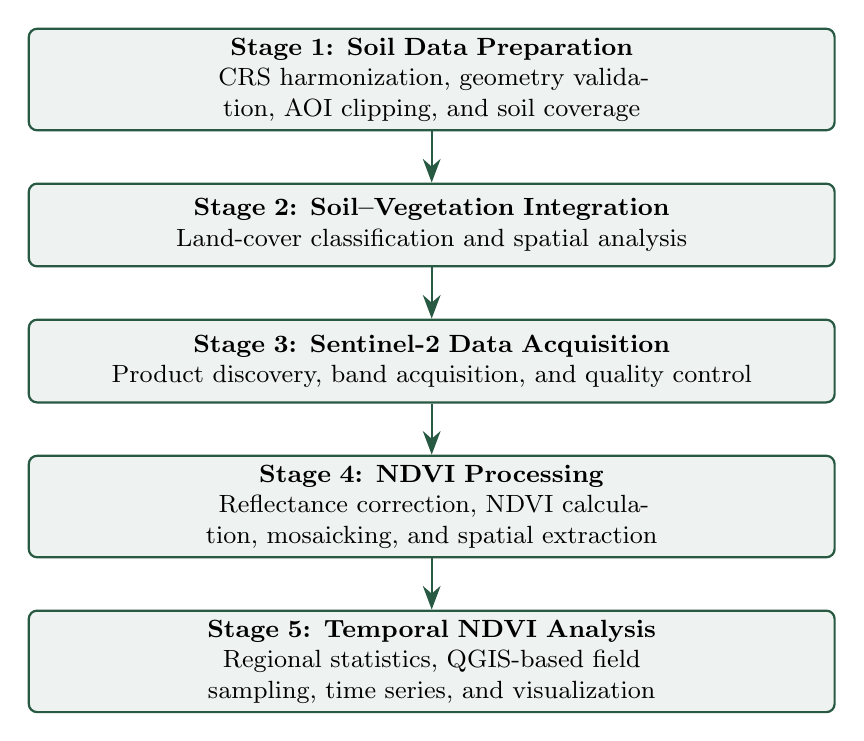
\begin{tikzpicture}[
	node distance=0.65cm,
	workflow/.style={
		rectangle,
		rounded corners=3pt,
		draw=geosoilgreen,
		fill=geosoilgreen!8,
		line width=0.8pt,
		text width=10cm,
		minimum height=1.05cm,
		align=center,
		font=\small
	},
	arrow/.style={
		-{Stealth[length=3mm]},
		thick,
		draw=geosoilgreen
	}
	]
	
	\node[workflow] (soil) {
		\textbf{Stage 1: Soil Data Preparation}\\
		CRS harmonization, geometry validation,
		AOI clipping, and soil coverage
	};
	
	\node[workflow, below=of soil] (vegetation) {
		\textbf{Stage 2: Soil--Vegetation Integration}\\
		Land-cover classification and spatial analysis
	};
	
	\node[workflow, below=of vegetation] (acquisition) {
		\textbf{Stage 3: Sentinel-2 Data Acquisition}\\
		Product discovery, band acquisition,
		and quality control
	};
	
	\node[workflow, below=of acquisition] (ndvi) {
		\textbf{Stage 4: NDVI Processing}\\
		Reflectance correction, NDVI calculation,
		mosaicking, and spatial extraction
	};
	
\node[workflow, below=of ndvi] (temporal) {
	\textbf{Stage 5: Temporal NDVI Analysis}\\
	Regional statistics, QGIS-based field sampling,
	time series, and visualization
};
	
	\draw[arrow] (soil) -- (vegetation);
	\draw[arrow] (vegetation) -- (acquisition);
	\draw[arrow] (acquisition) -- (ndvi);
	\draw[arrow] (ndvi) -- (temporal);
	
\end{tikzpicture}
	\caption{
		Simplified GeoSoil-Cuba workflow showing
		the principal stages of spatial data
		preparation, integration, and NDVI analysis.
	}
	\label{fig:workflow}
\end{figure}

The workflow comprises five principal stages:
soil-data inspection and preparation; soil-map
intersection with the Area of Interest (AOI);
integration of soil and vegetation information;
acquisition and quality screening of Sentinel-2
imagery; and calculation and analysis of NDVI.

The stages were implemented through a series
of Python notebooks, with QGIS used for the
visual selection of agricultural sampling areas.
Intermediate spatial datasets, tables, and
figures were exported to support quality control,
reproducibility, and subsequent analysis.


\subsection{Soil Data Preparation and AOI Intersection}
\label{subsec:soil-preparation}

The Mayabeque soil map at a scale of 1:25,000
was inspected before spatial analysis. The soil
dataset and the AOI were evaluated for their
coordinate reference systems and geometry
characteristics.

The AOI, originally supplied in WGS 84 geographic
coordinates (EPSG:4326), was transformed to
NAD27 / Cuba Norte (EPSG:3795), the projected
coordinate reference system used for soil-map
analysis.

Soil geometries were checked for validity.
Invalid geometries were repaired using
\texttt{make\_valid()}, and resulting geometry
collections were normalized to polygonal
geometries where necessary. The original source
data were preserved, and repaired geometries
were stored separately for analysis.

Soil features intersecting the AOI were selected
and clipped to its boundary. The resulting
dataset was used to assess soil-map coverage
and calculate the areas represented by mapped
soil units.

Spatial differences between the AOI and the
mapped soil coverage were examined alongside
the water-body dataset to distinguish
reservoir-related areas from other uncovered
locations.

Areas not represented by soil polygons and not
explained by the mapped reservoir were retained
as unresolved data gaps. No soil classifications
were assigned to these areas without supporting
information.

The resulting soil dataset was also examined
for undefined classification attributes and
overlapping polygon geometries. These conditions
were documented as data-quality findings.
Positive-area overlaps were identified but
were not automatically eliminated by modifying
the original soil-unit boundaries.


\subsection{Soil--Vegetation Integration}
\label{subsec:soil-vegetation-integration}

The processed soil layer was integrated with
existing vegetation and land-cover information
to support spatial analysis of mapped soil units
in their vegetation context.

The attributes \texttt{LCNAME}, \texttt{NEWVEG},
and \texttt{TNC\_CLASS} were retained for
analysis. Missing or undefined classification
values were identified during data preparation
rather than being replaced with unsupported
categories.

The integrated vector dataset provides a common
spatial framework for examining the distribution
of vegetation classifications across mapped
soil units. It also supports the preparation
of thematic maps and the examination of spatial
coverage and classification completeness.

The resulting dataset was exported in GeoPackage
format for subsequent analysis and cartographic
representation. The integration of these
datasets does not, by itself, establish
statistical or causal relationships between
soil properties and vegetation conditions.


\subsection{Sentinel-2 Acquisition and Quality Screening}
\label{subsec:sentinel-acquisition}

Sentinel-2 Level-2A imagery was obtained through
the Copernicus Data Space Ecosystem (CDSE) for
the period November 2025 to June 2026. Products
were discovered through the SpatioTemporal Asset
Catalog (STAC) interface using the geographic
extent and acquisition period relevant to the
study area.

The study area intersects Sentinel-2 tiles
T17QLF and T17QMF. The red band (B04) and
near-infrared band (B08), both provided at
10 m spatial resolution, were selected for
NDVI calculation.

Acquisition records were organized by date,
satellite, and tile to identify complete B04/B08
pairs. Incomplete band pairs were excluded
from NDVI processing.

The Scene Classification Layer (SCL), provided
at 20 m spatial resolution, was used to support
quality screening for potentially cloud- and
shadow-contaminated observations.

The initial satellite inventory contained
226 observations. Following tile-level processing
and preparation of the agricultural analysis
region, 32 acquisition dates were represented
by analysis-area NDVI rasters. A subsequent
regional cloud-screening procedure retained
15 acquisitions meeting the final criterion
of less than 10\% cloud coverage within the
agricultural analysis region.

The cloud-coverage threshold was used as an
acquisition-selection criterion. It does not
guarantee that all pixels in the retained
observations are free from clouds, haze, or
shadows. Cloud screening and numerical NDVI
validation were therefore treated as distinct
quality-control procedures.

Regional cloud coverage was calculated
using SCL classes 8, 9, and 10,
representing medium-probability clouds,
high-probability clouds, and thin cirrus,
respectively.

Cloud shadows, represented by SCL
class 3, were evaluated separately
and were not included in the reported
cloud-coverage percentage.

\subsection{Radiometric Correction and NDVI Calculation}
\label{subsec:ndvi-method}

Sentinel-2 Level-2A spectral bands are distributed
as integer digital numbers (DN). Bottom-of-atmosphere
(BOA) reflectance was calculated using the
radiometric quantification value and additive
offset associated with the satellite products:

\begin{equation}
	\rho_{\mathrm{BOA}} =
	\frac{DN + O_{\mathrm{BOA}}}{Q_{\mathrm{BOA}}},
	\label{eq:boa-reflectance}
\end{equation}

where $DN$ represents the stored pixel value,
$O_{\mathrm{BOA}}$ is the additive radiometric
offset, and $Q_{\mathrm{BOA}}$ is the reflectance
quantification value.

An examination of 111 available Sentinel-2
product XML metadata files identified a
quantification value of 10,000 and additive
offsets of $-1000$ for both B04 and B08.
The examined products corresponded to
processing baselines 05.11 and 05.12.

For consistency, these parameters were applied
to all images used in the analysis, including
products for which XML metadata were unavailable.
Consequently, the radiometric parameters were
not independently verified for every processed
image.

Under this assumption, reflectance was calculated
as:

\begin{equation}
	\rho_{\mathrm{BOA}} =
	\frac{DN - 1000}{10000}.
	\label{eq:boa-correction}
\end{equation}

The Normalized Difference Vegetation Index
(NDVI) was calculated from the corrected red
and near-infrared reflectance values:

\begin{equation}
	\mathrm{NDVI} =
	\frac{\rho_{\mathrm{B08}}-\rho_{\mathrm{B04}}}
	{\rho_{\mathrm{B08}}+\rho_{\mathrm{B04}}},
	\label{eq:ndvi}
\end{equation}

where $\rho_{\mathrm{B08}}$ represents
near-infrared BOA reflectance and
$\rho_{\mathrm{B04}}$ represents red BOA
reflectance.

The additive radiometric offsets were applied
before NDVI calculation. Although a common
multiplicative factor cancels in the normalized
difference, an additive offset does not.
Consequently, the treatment of the additive
offset affects the calculated NDVI values.

Pixels containing zero digital numbers,
nonfinite values, negative corrected reflectance,
or nonpositive reflectance sums were excluded.
Calculated NDVI values outside the theoretical
interval $[-1,1]$ were also rejected.

Invalid pixels were assigned a NoData value
of $-9999$. The resulting NDVI rasters were
exported as single-band, 32-bit floating-point
GeoTIFF files.


\subsection{NDVI Mosaicking and Spatial Extraction}
\label{subsec:ndvi-processing}

NDVI was initially calculated independently
for each complete Sentinel-2 B04/B08 tile pair.

For acquisition dates with both required tiles,
the corresponding tile-level NDVI rasters from
T17QLF and T17QMF were mosaicked to provide
spatial coverage across the analysis region.

The agricultural analysis region was defined
using five polygons from the integrated
soil--vegetation dataset.

Four polygons were associated with
Ferralítico Rojo Típico
(Typical Red Ferrallitic Soil), and
one was associated with
Ferralítico Amarillento Típico
(Typical Yellowish Ferrallitic Soil).

The selected polygons were combined
into a unified analysis geometry
covering approximately 16.22~km$^2$.
This geometry was used consistently
for regional NDVI extraction across
the selected Sentinel-2 acquisitions.

The geometry of the selected agricultural
analysis region was used to define the
extraction area. The relevant vector geometry
was transformed from EPSG:3795 to EPSG:32617,
the coordinate reference system of the
Sentinel-2 rasters, before spatial extraction.

The mosaics were cropped to the analysis
geometry and exported as GeoTIFF files at
10 m spatial resolution.

The processing inventory contained 64
tile-level NDVI rasters and 32 analysis-area
NDVI rasters, corresponding to 32 acquisition
dates. These counts describe the processed
inventory before the final regional cloud
screening used to select the 15 acquisitions
for temporal analysis.


\subsection{QGIS-Based Selection of Potato Fields}
\label{subsec:qgis-potato-fields}

QGIS was used to identify three potato fields
within the processed agricultural region.
The selected locations were verified using
local knowledge of the study area and were
used for a more focused examination of
vegetation-index variability.

The sampling areas were digitized as three
separate circular polygons and overlaid on
the processed NDVI rasters for visual
inspection. These polygons represent
selected sampling areas rather than surveyed
field boundaries.

The same three sampling polygons were used
to extract NDVI observations for the available
acquisition dates, allowing temporal
comparisons within and between the sampled
areas.

The field-level dataset contained 45
field-date observations, corresponding to
three sampling areas evaluated over 15
Sentinel-2 acquisition dates. For each
sampling area and date, the extracted data
were summarized using the number of valid
pixels, mean NDVI, median NDVI, and standard
deviation.

The resulting dataset supports comparisons
of temporal NDVI patterns among the three
sampled areas. Because the sampling polygons
represent selected locations rather than
a comprehensive survey of potato cultivation,
the results should not be interpreted as
representative of every potato field in
the study region.


\subsection{Raster Validation and Temporal Sampling}
\label{subsec:raster-validation}

The analysis-area NDVI rasters were validated
to assess their spatial and numerical
consistency.

Validation included checks of the coordinate
reference system, spatial resolution, raster
dimensions, data type, number of bands,
NoData representation, and range of valid
NDVI values.

The expected raster characteristics were
EPSG:32617, 10 m spatial resolution, a single
32-bit floating-point band, and a NoData
value of $-9999$. Valid NDVI values were
required to fall within the interval $[-1,1]$.

A 15-date temporal sampling design was used
to examine vegetation-index variability across
three broad periods: November--February,
March--April, and May--June. Candidate
acquisitions were evaluated according to
temporal distribution and the availability
of suitable observations.

Only dates represented by processed and
validated imagery were included in the
subsequent temporal analysis.


\subsection{Temporal and Agricultural-Region Analysis}
\label{subsec:temporal-analysis}

The accepted NDVI observations were analyzed
to characterize temporal variation in
vegetation-index values within the agricultural
analysis region and the three selected
sampling areas.

Regional NDVI summaries were used to examine
changes across acquisition dates. Field-level
summaries were used to compare the mean,
median, and variability of NDVI within each
sampling polygon over the same observation
period.

Tables and plots were generated to examine
temporal trends and differences among
the sampled areas. The analysis was
descriptive and focused on the distribution
and evolution of satellite-derived NDVI
values.

The resulting observations provide information
about vegetation-index variability during
the study period. They are not direct
measurements of crop yield, soil properties,
or agricultural management, and they do not
independently establish the causes of
observed temporal changes.
	\section{Results}
\label{sec:results}

The GeoSoil-Cuba workflow produced validated spatial
datasets, satellite-derived vegetation indices, and
statistical summaries describing soil-map coverage
and vegetation variability within the study area.

The results are organized into eight subsections
covering soil topology, spatial coverage, satellite
acquisition screening, preliminary NDVI inspection,
agricultural-region selection, temporal variability,
spatial NDVI distributions, and field-level observations.


\subsection{Soil Topology and Area-Accounting Validation}
\label{subsec:topology_validation}

The topology assessment identified differences between
the summed areas of individual clipped soil polygons
and the area of their geometric union. These
measurements were compared in the source coordinate
reference system (EPSG:3795) and after reprojection
to UTM Zone 17N (EPSG:32617).

In EPSG:3795, the sum of all clipped soil polygon
areas was 162.907~km$^2$, comprising
161.984~km$^2$ of classified soil polygons and
0.922~km$^2$ associated with an undefined
classification. The corresponding geometric union
covered 162.852~km$^2$, yielding a difference
of approximately 0.055~km$^2$.

After reprojection to EPSG:32617, the sum of all
polygon areas decreased to 162.820~km$^2$,
comprising 161.899~km$^2$ of classified soil
polygons and 0.922~km$^2$ associated with the
undefined classification. The geometric union
covered 162.766~km$^2$, again yielding a
difference of approximately 0.055~km$^2$.

The total polygon-area sum decreased by
0.086~km$^2$ (approximately 0.053\%)
between the two CRSs. The geometric union
area decreased by a similar amount, while
the difference between the polygon-area sum
and the geometric union remained nearly
unchanged. These results demonstrate the
sensitivity of planar area measurements to
coordinate reference system transformations,
while confirming that the overlap-related
area difference was consistent between
the two CRSs.

Pairwise intersection analysis identified
90 polygon pairs with positive-area overlaps.
Their cumulative pairwise overlap area was
0.054919~km$^2$, representing approximately
0.034\% of the summed polygon area in
EPSG:32617.

The largest individual overlap measured
0.046807~km$^2$ and occurred between
Aluvial Poco Diferenciado (2618) and
Pardo con Carbonatos Típico (1001).

The principal area-accounting and topology
results are summarized in
\Cref{tab:soil_topology_validation}.

\begin{table}[htbp]
	\centering
	\caption{
		Soil polygon area accounting and
		topology validation results.
	}
	\label{tab:soil_topology_validation}
	\small
	
	\begin{tabular}{lr}
		\hline
		\textbf{Metric} & \textbf{Value} \\
		\hline
		
		\multicolumn{2}{l}{
			\textit{Area measurements in EPSG:3795}
		} \\
		\hline
		
		Classified soil polygon-area sum (km$^2$)
		& 161.984 \\
		
		Undefined soil polygon area (km$^2$)
		& 0.922 \\
		
		Total polygon-area sum (km$^2$)
		& 162.907 \\
		
		Geometric union area (km$^2$)
		& 162.852 \\
		
		Sum minus union (km$^2$)
		& 0.055 \\
		
		\hline
		\multicolumn{2}{l}{
			\textit{Area measurements in EPSG:32617}
		} \\
		\hline
		
		Classified soil polygon-area sum (km$^2$)
		& 161.899 \\
		
		Undefined soil polygon area (km$^2$)
		& 0.922 \\
		
		Total polygon-area sum (km$^2$)
		& 162.820 \\
		
		Geometric union area (km$^2$)
		& 162.766 \\
		
		Sum minus union (km$^2$)
		& 0.055 \\
		
		\hline
		\multicolumn{2}{l}{
			\textit{CRS comparison}
		} \\
		\hline
		
		Change in polygon-area sum (km$^2$)
		& $-0.086$ \\
		
		Relative change in polygon-area sum (\%)
		& $-0.053$ \\
		
		\hline
		\multicolumn{2}{l}{
			\textit{Topology validation}
		} \\
		\hline
		
		Overlapping polygon pairs
		& 90 \\
		
		Total pairwise overlap area (km$^2$)
		& 0.054919 \\
		
		Largest individual overlap (km$^2$)
		& 0.046807 \\
		
		Pairwise overlap / total polygon area (\%)
		& 0.034 \\
		
		\hline
	\end{tabular}
\end{table}

The cumulative pairwise overlap area closely
matched the difference between the summed
polygon areas and their geometric union in
EPSG:32617. Specifically, the sum-minus-union
difference was 0.054919~km$^2$, matching the
reported cumulative pairwise overlap area
to six decimal places.

However, pairwise overlap calculations may
count the same location more than once where
three or more polygons intersect. Consequently,
the cumulative pairwise overlap area should
not be interpreted as an exact measure of
the geographic area affected by overlaps.
Likewise, the difference between the polygon-area
sum and the geometric union represents excess
area arising from overlapping polygons rather
than necessarily the unique geographic extent
of the overlapping regions.

The detected overlaps were retained as
data-quality findings. No source soil-unit
boundaries were modified or removed to
eliminate these intersections.

\subsection{Soil and Vegetation Spatial Coverage}
\label{subsec:spatial_results}

The Area of Interest (AOI) covers approximately
178.47~km$^2$. The spatial coverage assessment
reported soil-map coverage of approximately
162.85~km$^2$, equivalent to 91.25\% of the AOI.

The corresponding uncovered area was
15.62~km$^2$, representing approximately
8.75\% of the AOI.

Water bodies occupied approximately
14.49~km$^2$ within the AOI. Of this area,
approximately 3.07~km$^2$ overlapped
existing soil polygons, while
11.42~km$^2$ was not covered by the
soil dataset.

The remaining non-water gaps accounted for
approximately 4.20~km$^2$, equivalent
to 2.35\% of the AOI.

The principal spatial coverage measurements
are presented in \Cref{tab:spatial_coverage}.

\begin{table}[htbp]
	\centering
	\caption{
		Reported spatial coverage of soil,
		water-body, and vegetation datasets
		within the Area of Interest.
	}
	\label{tab:spatial_coverage}
	
	\begin{tabular}{lrr}
		\hline
		
		\textbf{Spatial component} &
		\textbf{Area (km$^2$)} &
		\textbf{AOI (\%)} \\
		
		\hline
		
		Area of Interest
		& 178.47 & 100.00 \\
		
		Soil-map coverage
		& 162.85 & 91.25 \\
		
		Total soil-data gap
		& 15.62 & 8.75 \\
		
		Water-body area
		& 14.49 & 8.12 \\
		
		Water area not covered by soil polygons
		& 11.42 & 6.40 \\
		
		Remaining non-water gaps
		& 4.20 & 2.35 \\
		
		Vegetation coverage
		& 161.93 & 90.73 \\
		
		\hline
	\end{tabular}
\end{table}

The soil-map coverage reported in
\Cref{tab:spatial_coverage} differs slightly
from the geometric union area reported in
\Cref{tab:soil_topology_validation}.

The two measurements are therefore retained
as distinct reported results. Their difference
requires verification against the processing
stages and geometry sets used to calculate
the respective areas.

The spatial distribution of the remaining
soil-data gaps is shown in
\Cref{fig:remaining_soil_gaps}.

\begin{figure}[htbp]
	\centering
	
	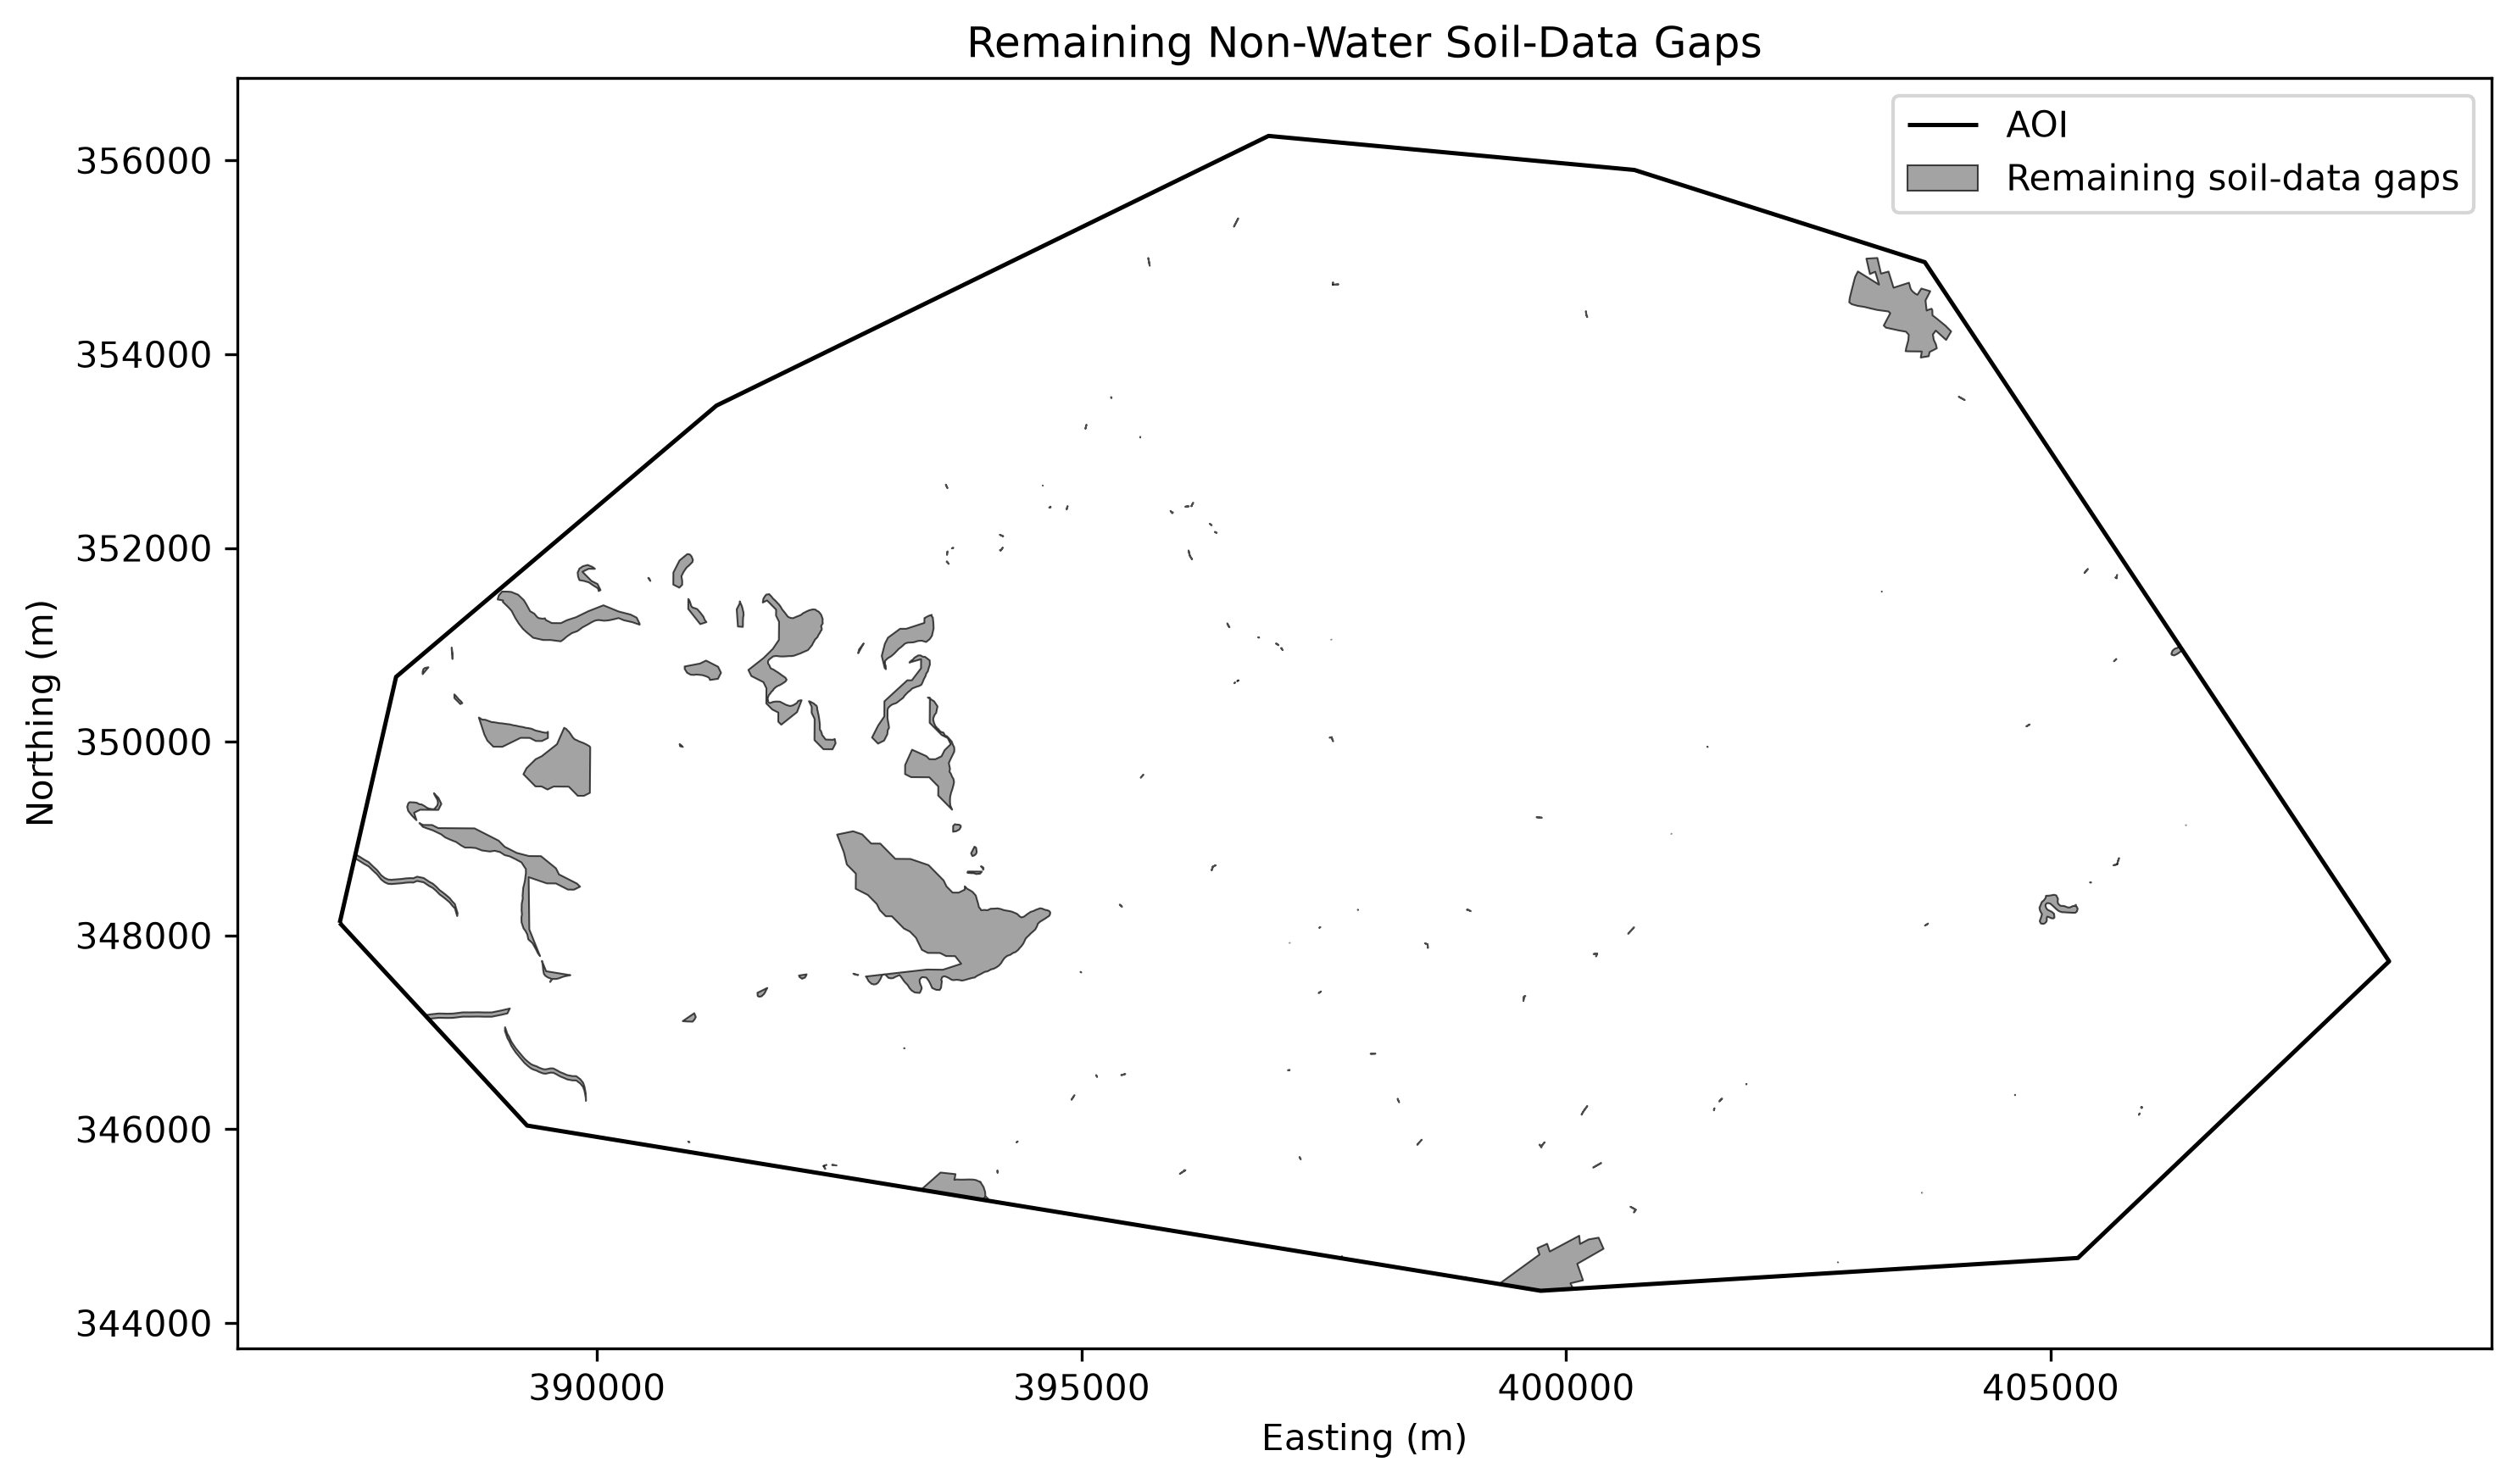
\includegraphics[
	width=0.90\linewidth
	]{../figures/remaining_soil_data_gaps.png}
	
	\caption{
		Spatial distribution of remaining
		areas without soil-map coverage
		within the AOI, following the
		identification of water-related
		gaps associated with the
		Mampostón reservoir.
	}
	
	\label{fig:remaining_soil_gaps}
\end{figure}

The clipped soil inventory contained one
polygon with the attribute combination
\texttt{Cód\_tipo = 0} and
\texttt{Cód\_stipo = 0}.

Because code zero was not defined as a
valid soil type or subtype in Anexo~6,
the polygon was classified as undefined
rather than assigned to an unsupported
soil category.

This polygon accounted for
0.922~km$^2$ of the summed soil
polygon area.

The spatial distribution of the mapped
soil units is presented in
\Cref{fig:soil_vegetation}.

\begin{figure}[htbp]
	\centering
	
	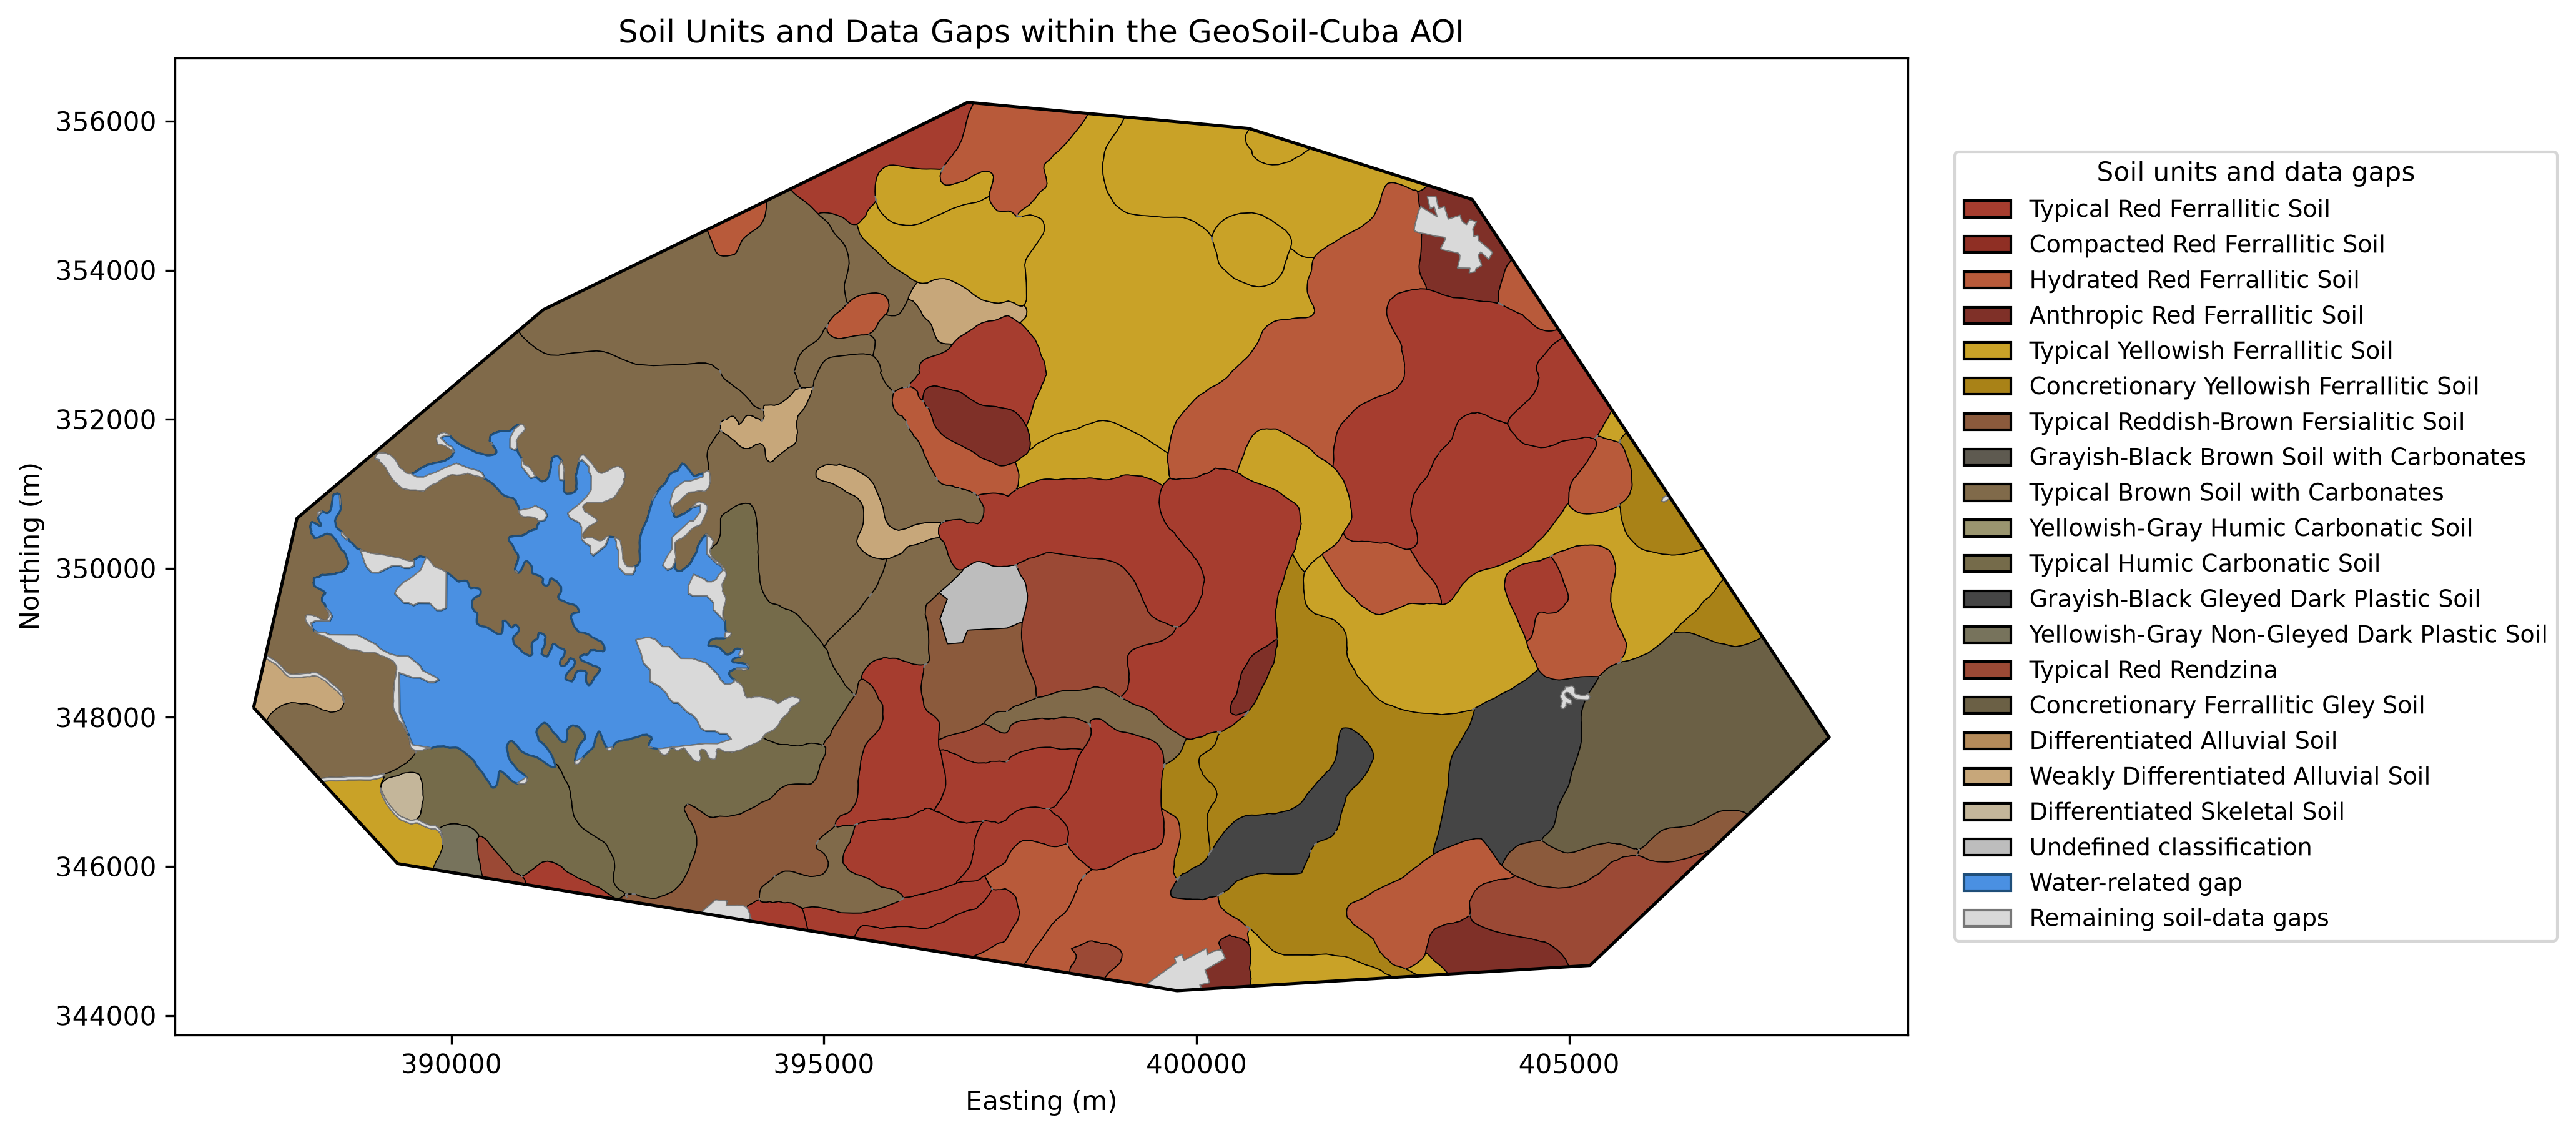
\includegraphics[
	width=\linewidth
	]{../figures/soil_units_aoi.png}
	
	\caption{
		Spatial distribution of mapped
		soil units within the AOI,
		including areas with undefined
		soil classification.
	}
	
	\label{fig:soil_vegetation}
\end{figure}

The vegetation and land-cover dataset
provided reported spatial coverage of
approximately 161.93~km$^2$.

The inventory included grasslands
(87.45~km$^2$), cultivated land
(75.86~km$^2$), secondary vegetation
(13.69~km$^2$), and flooded hydromorphic
areas (1.47~km$^2$).

The sum of these reported class areas
exceeds the stated vegetation coverage.
Consequently, these measurements cannot
be interpreted as a mutually exclusive
partition of the vegetation-covered area
without further verification of the
classification and area-accounting methods.

The spatial distribution of the vegetation
categories is illustrated in
\Cref{fig:vegetation_types}.

\begin{figure}[htbp]
	\centering
	
	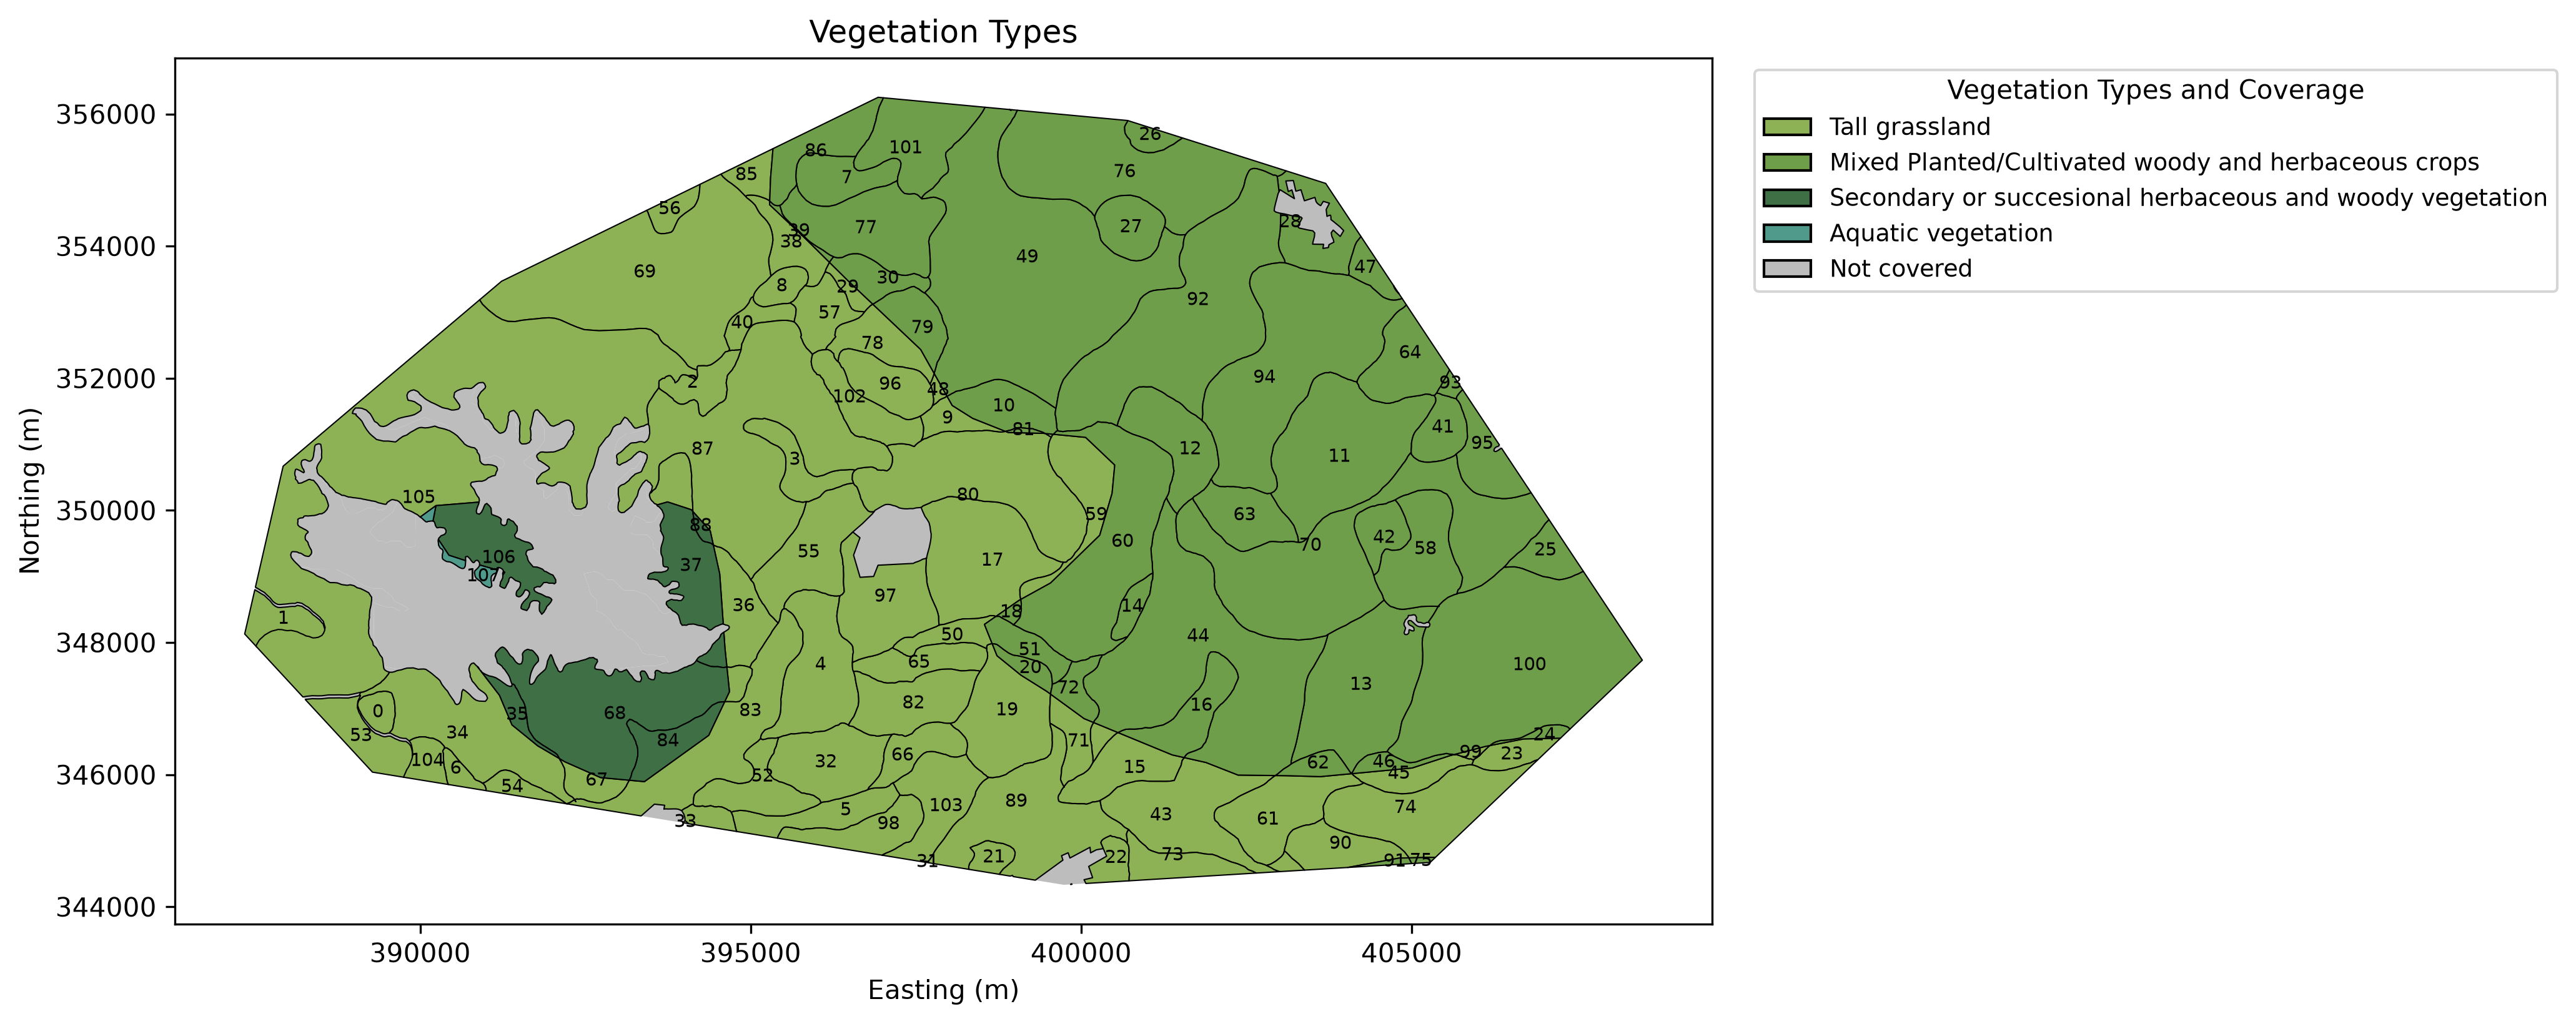
\includegraphics[
	width=\linewidth
	]{../figures/vegetation_types.png}
	
	\caption{
		Spatial distribution of mapped
		vegetation and land-cover
		categories within the AOI.
	}
	
	\label{fig:vegetation_types}
\end{figure}

These spatial datasets provided the basis
for integrating soil classifications with
existing vegetation and land-cover
information.


\subsection{Sentinel-2 Acquisition and Quality Screening}
\label{subsec:sentinel_results}

The Sentinel-2 inventory contained
226 observations acquired between
November 2025 and June 2026.

The mean catalogue-reported cloud-cover
percentage was 40.04\%, indicating
substantial variation in acquisition
conditions across the available imagery.

Following satellite processing,
32 NDVI rasters were generated for
the selected agricultural region.

The regional quality-screening procedure
retained 15 acquisitions with less
than 10\% cloud coverage within the
analysis region.

The accepted observations spanned
3 November 2025 to 16 June 2026.

The temporal distribution of these
acquisitions was not uniform, reflecting
the availability of observations meeting
the regional screening criterion.

Fourteen retained rasters contained
162,195 valid NDVI pixels, while one
contained 162,193 valid pixels.

The nearly constant valid-pixel counts
indicate that the accepted rasters
represented a stable spatial sampling
extent, although this numerical
consistency does not independently
establish the absence of residual
cloud or shadow contamination.


\subsection{Initial Inspection of NDVI Data}
\label{subsec:initial_ndvi_inspection}

A preliminary inspection was conducted
using 14 NDVI rasters from the available
Sentinel-2 observations.

The initial analysis examined spatial
NDVI patterns, temporal changes in
summary statistics, and differences
in pixel-level distributions.

A representative NDVI map from
3 November 2025 is presented in
\Cref{fig:initial_ndvi_map}.

\begin{figure}[htbp]
	\centering
	
	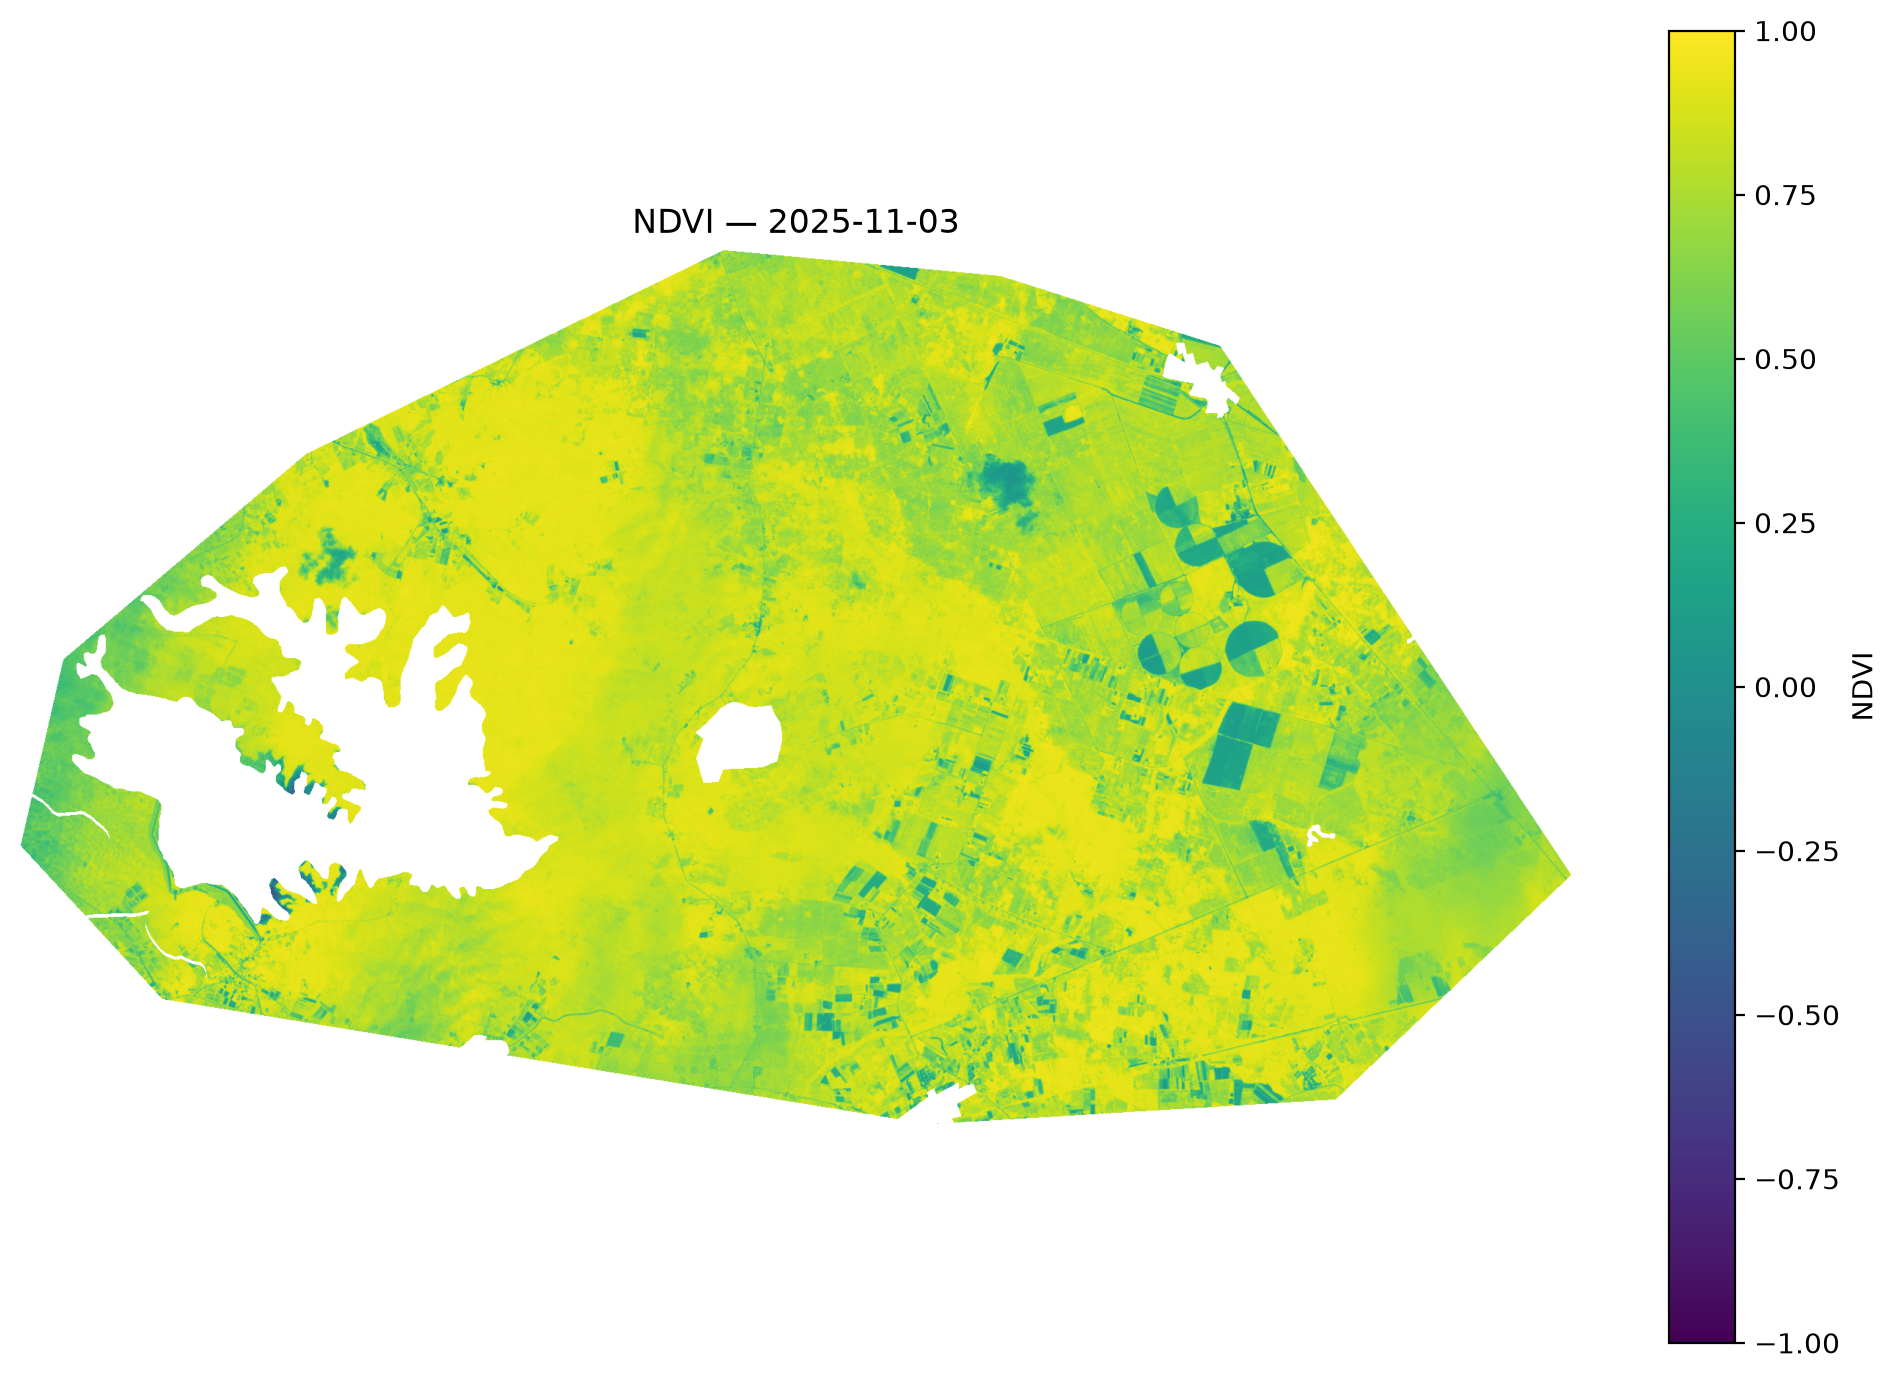
\includegraphics[
	width=0.90\linewidth
	]{../figures/stage5_figure_23.png}
	
	\caption{
		Preliminary NDVI map derived
		from Sentinel-2 imagery acquired
		on 3 November 2025.
	}
	
	\label{fig:initial_ndvi_map}
\end{figure}

The initial temporal summaries are
shown in \Cref{fig:initial_ndvi_timeseries},
while the corresponding pixel-level
distributions are presented in
\Cref{fig:initial_ndvi_boxplots}.

\begin{figure}[htbp]
	\centering
	
	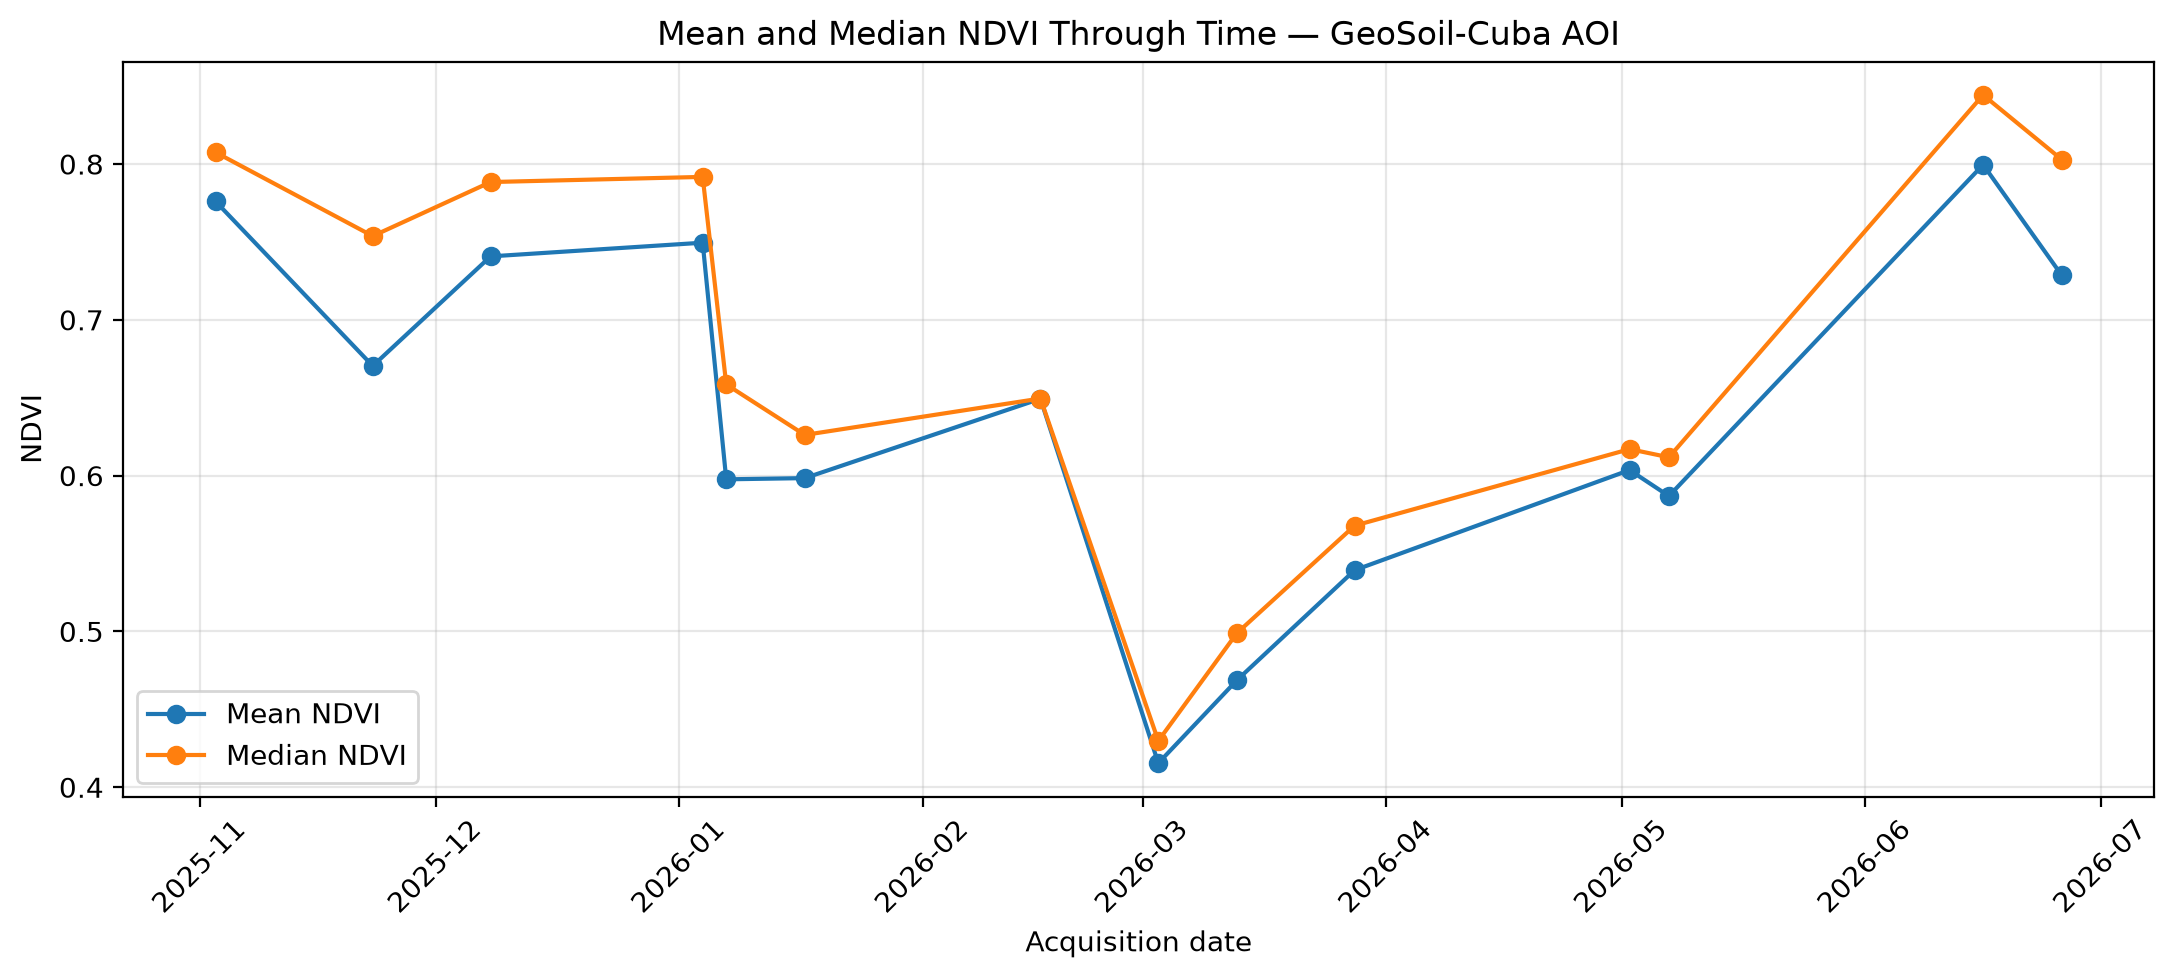
\includegraphics[
	width=0.90\linewidth
	]{../figures/stage5_figure_17.png}
	
	\caption{
		Preliminary temporal variation
		in mean and median NDVI across
		the initially selected raster
		observations.
	}
	
	\label{fig:initial_ndvi_timeseries}
\end{figure}

\begin{figure}[htbp]
	\centering
	
	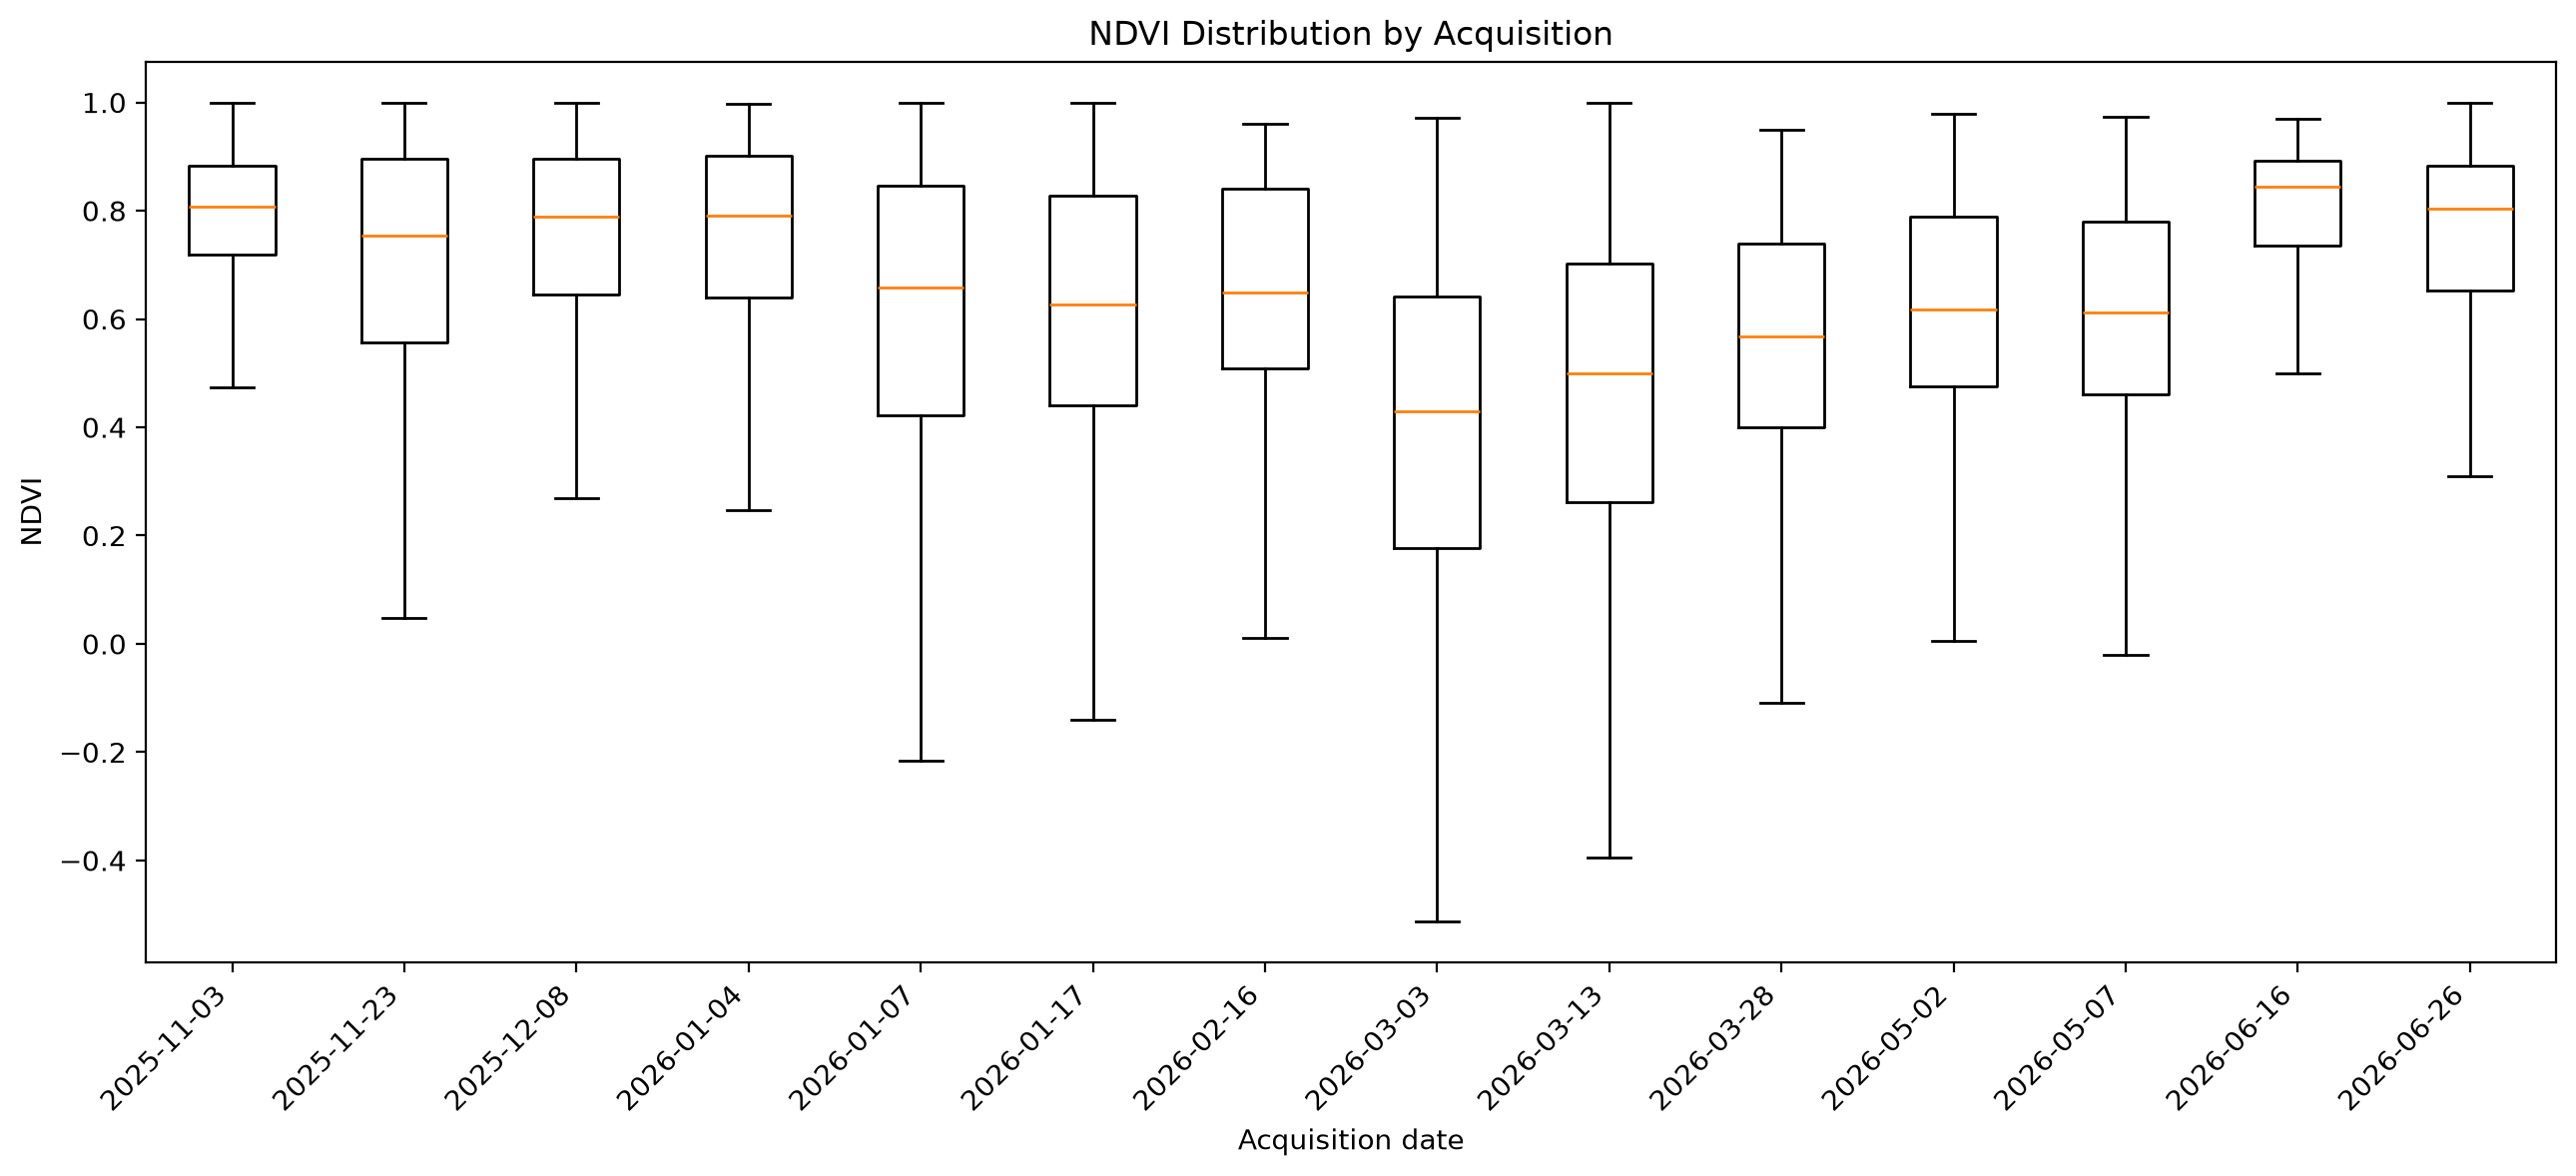
\includegraphics[
	width=0.90\linewidth
	]{../figures/stage5_figure_21.png}
	
	\caption{
		Preliminary distributions of
		pixel-level NDVI values across
		the initially selected
		Sentinel-2 observations.
	}
	
	\label{fig:initial_ndvi_boxplots}
\end{figure}

Inspection revealed that some rasters
provided incomplete spatial coverage
of the broader study area.

The incomplete coverage was associated
with limitations in the available
Sentinel-2 imagery rather than
with the mapped reservoir.

The subsequent agricultural analysis
region was located outside the
affected areas, allowing a consistent
spatial extent to be used for
the final temporal analysis.

The preliminary observations are
therefore presented as exploratory
results and are distinguished from
the final 15-acquisition analysis.


\subsection{Selection of the NDVI Analysis Region}
\label{subsec:ndvi_region_selection}

Five agricultural polygons were selected
from the integrated soil--vegetation
dataset and combined into a unified
analysis region.

Four polygons were associated with
Ferralítico Rojo Típico
(Typical Red Ferrallitic Soil), while
one was associated with
Ferralítico Amarillento Típico
(Typical Yellowish Ferrallitic Soil).

The resulting agricultural analysis
region covered approximately
16.22~km$^2$.

Its spatial distribution is presented
in \Cref{fig:ndvi_selected_region}.

\begin{figure}[htbp]
	\centering
	
	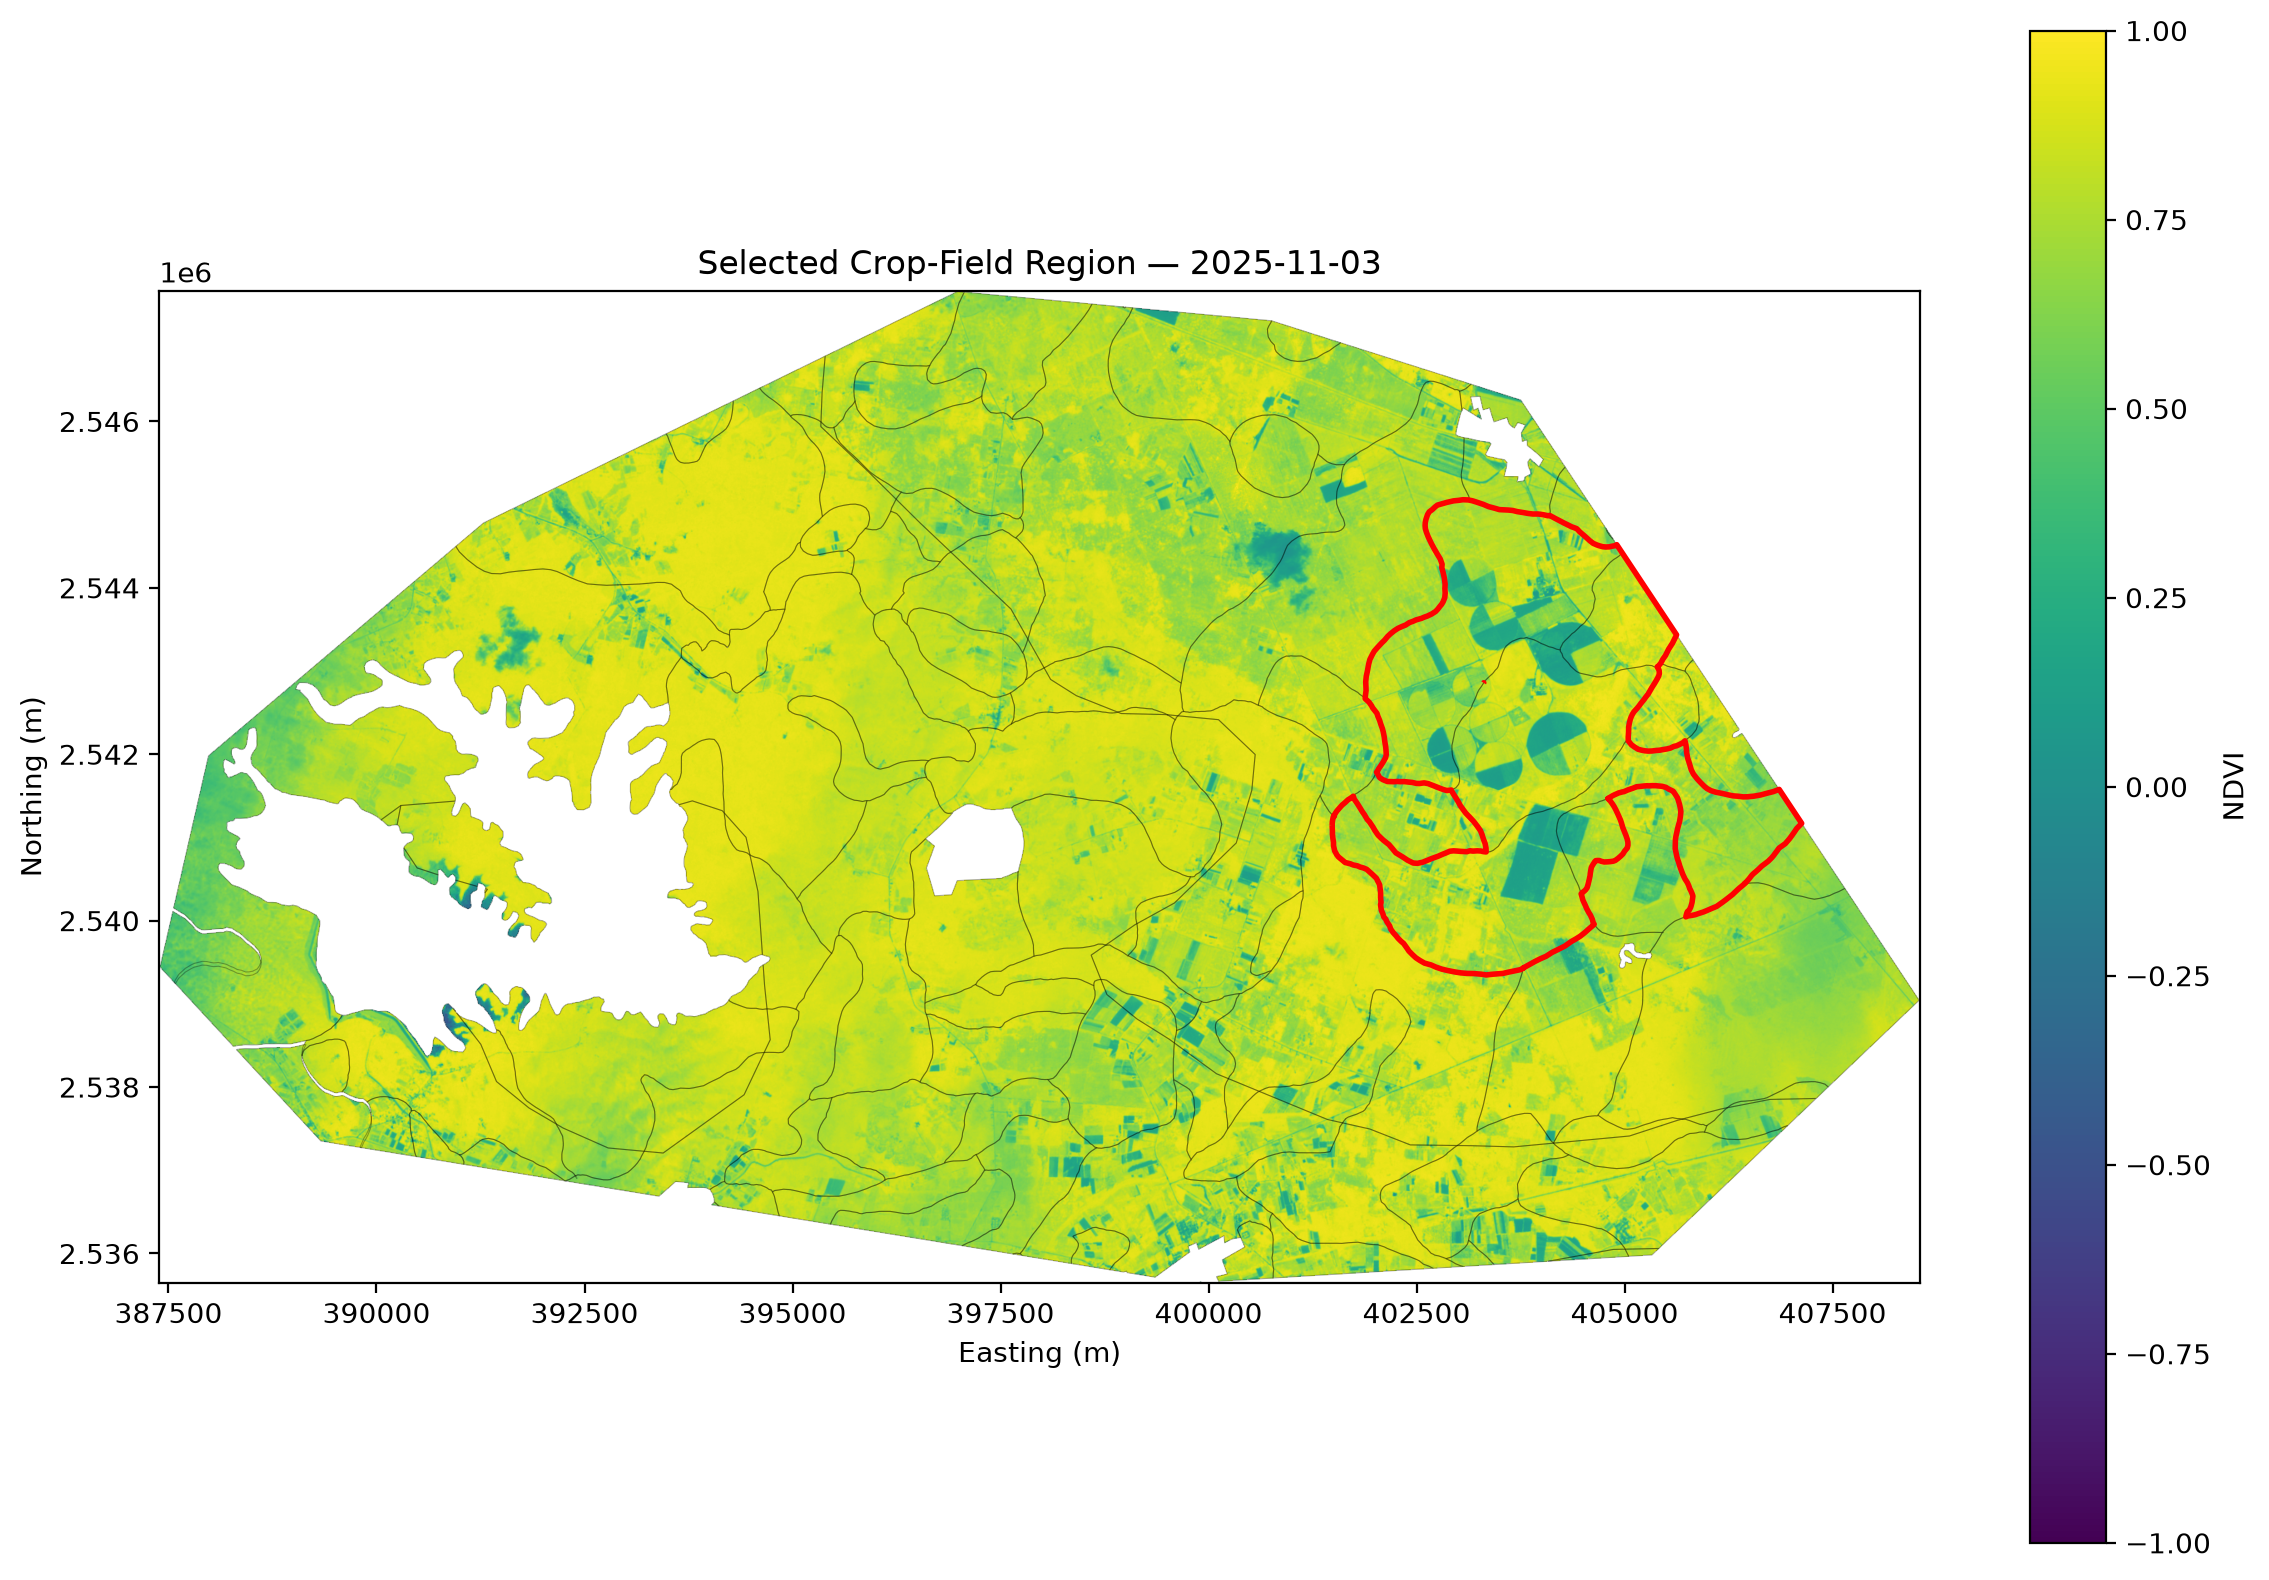
\includegraphics[
	width=0.90\linewidth
	]{../figures/stage5_figure_41.png}
	
	\caption{
		Spatial distribution of the five
		selected agricultural polygons
		and their unified analysis
		region within the study area.
	}
	
	\label{fig:ndvi_selected_region}
\end{figure}

The selected region was located
outside the areas affected by
incomplete satellite coverage
identified during the preliminary
inspection.

The 32 regional NDVI rasters
provided the initial image
collection for this area.

Following regional SCL-based
quality screening, 15 acquisitions
were retained for the temporal
and spatial NDVI analyses.

The retained acquisitions are
illustrated in
\Cref{fig:ndvi_cloud_screening}.

\begin{figure}[htbp]
	\centering
	
	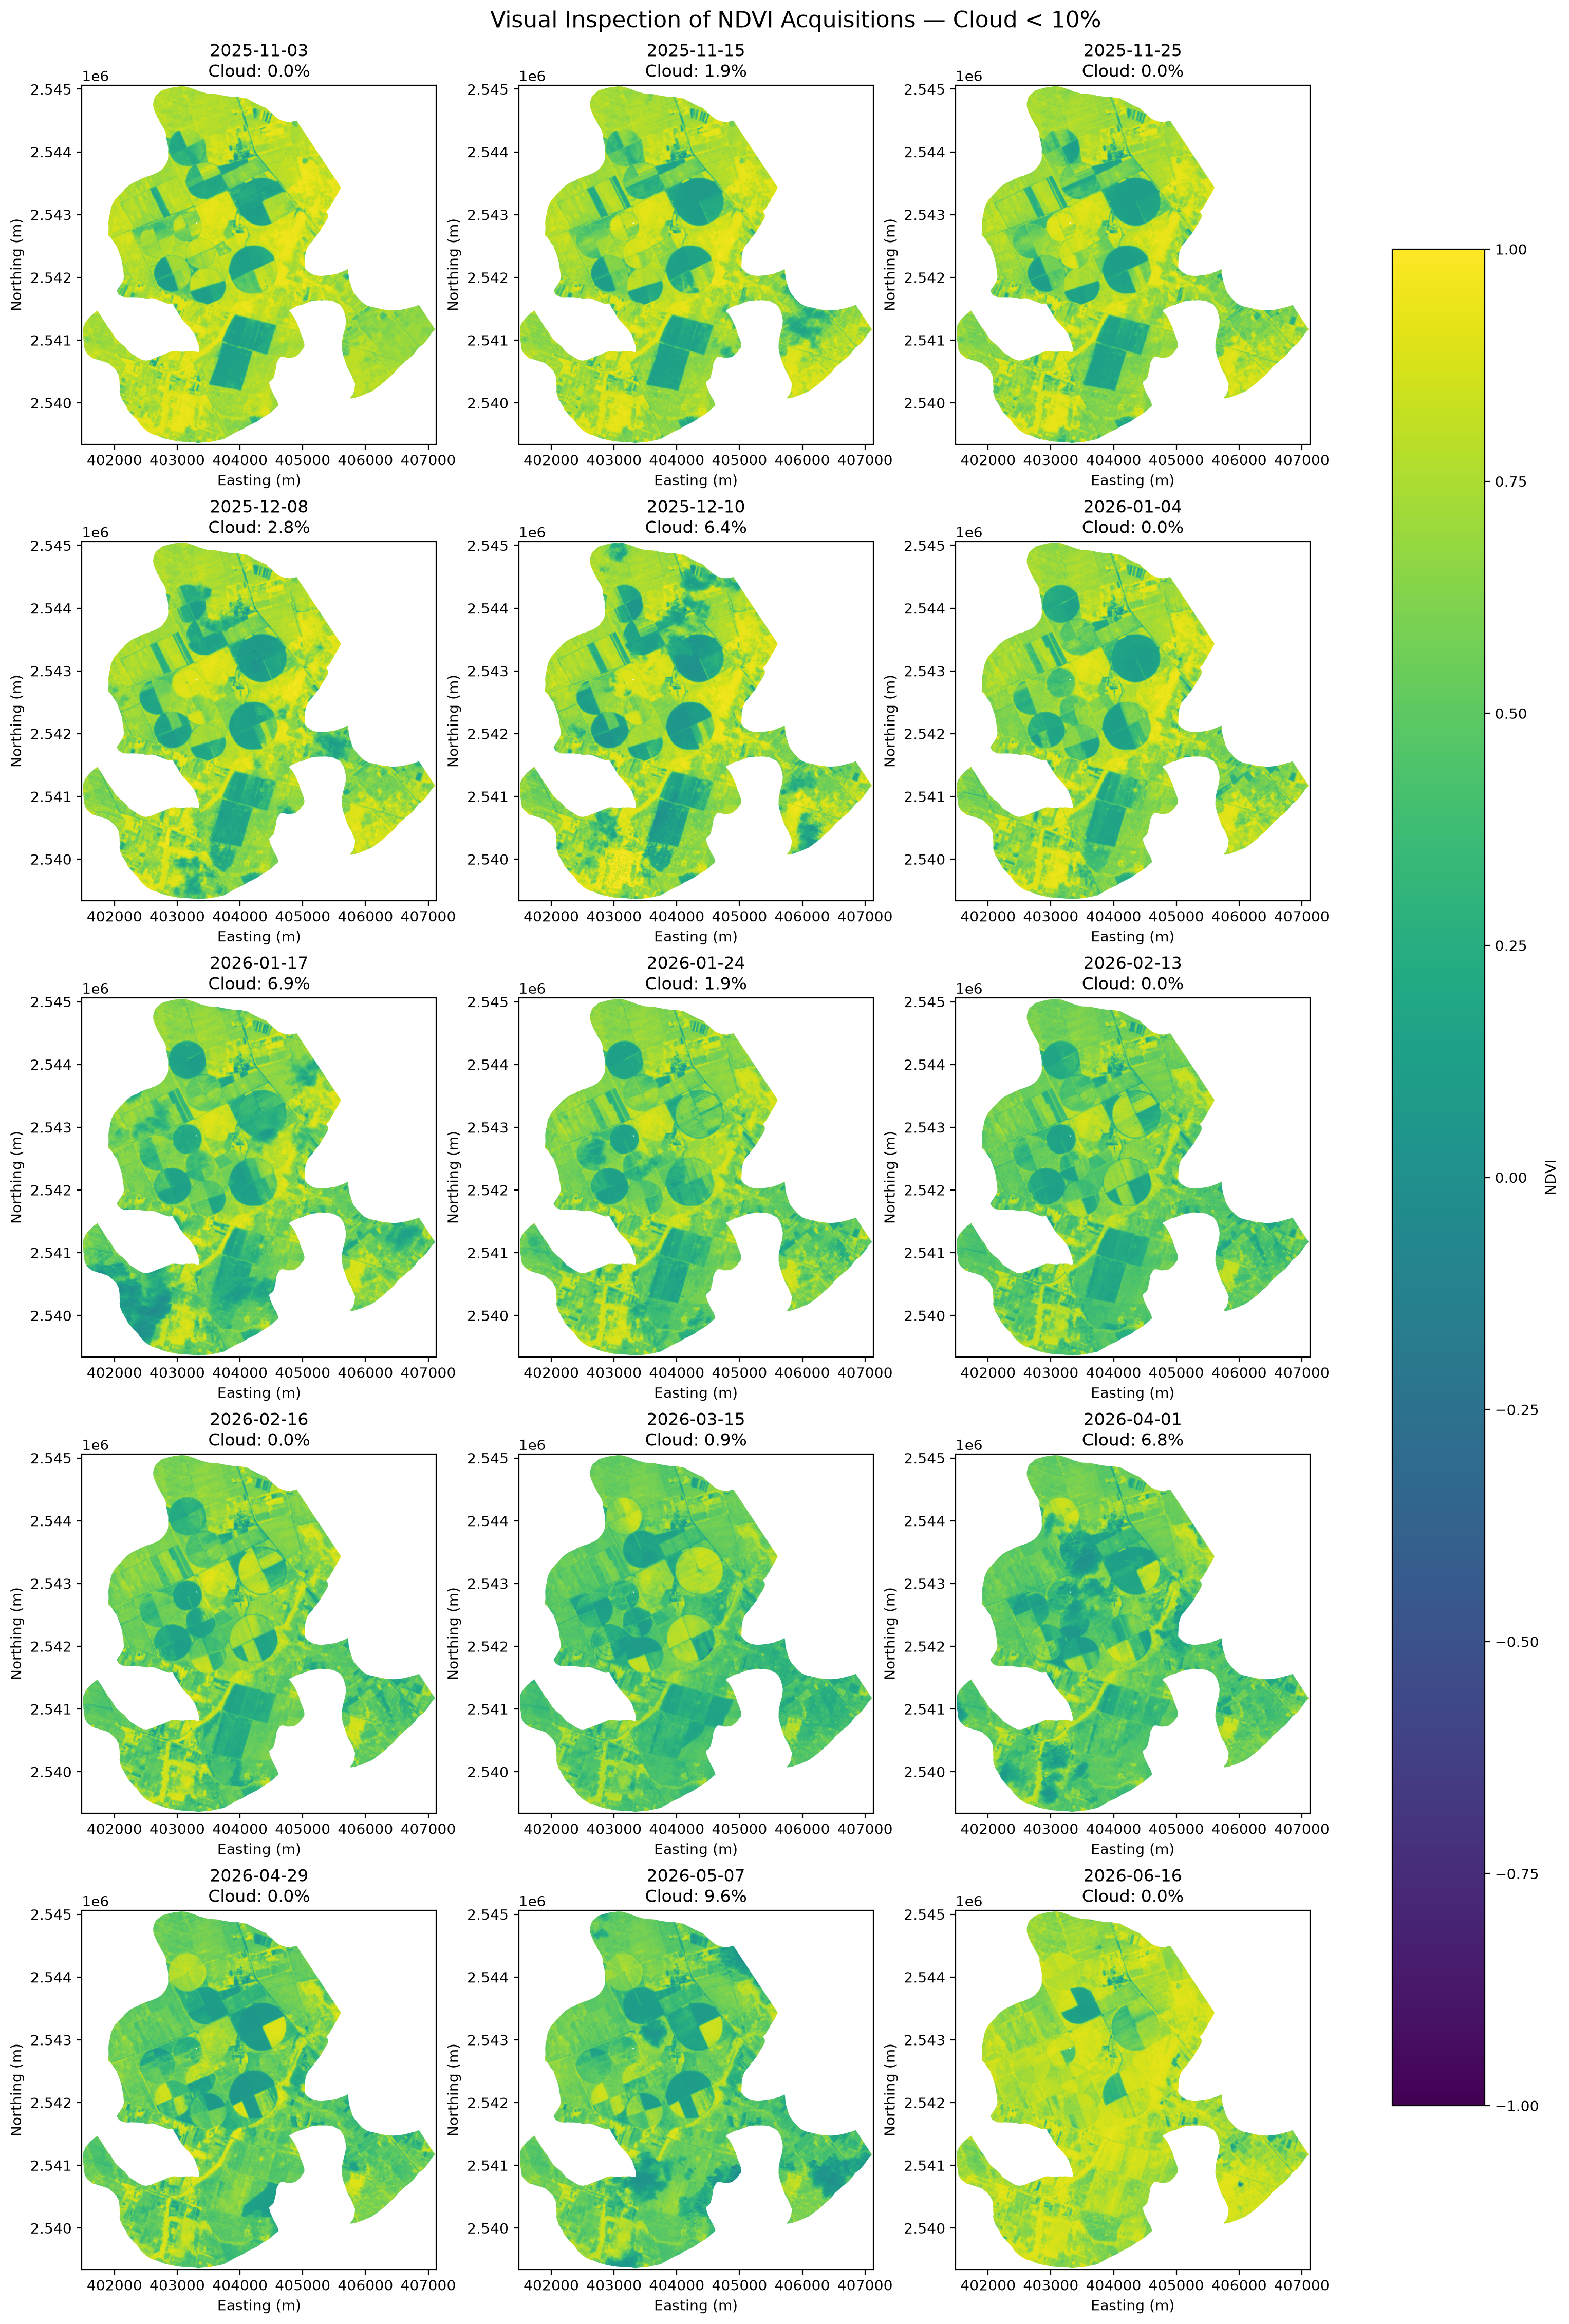
\includegraphics[
	width=\linewidth
	]{../figures/stage5_figure_59.png}
	
	\caption{
		Visual comparison of the
		15 regional NDVI acquisitions
		satisfying the cloud-coverage
		criterion of less than 10\%.
	}
	
	\label{fig:ndvi_cloud_screening}
\end{figure}

The unified region provided a
consistent geographic basis for
comparing vegetation-index
observations throughout the
study period.


\subsection{Temporal NDVI Variability}
\label{subsec:temporal_ndvi_variability}

Temporal NDVI variability was examined
using the mean and median values
calculated for the 15 accepted
Sentinel-2 acquisitions.

The results indicate a general
decline in regional NDVI from
November 2025 through March 2026.

Mean NDVI decreased from approximately
0.688 on 3 November 2025 to
0.466 on 15 March 2026.

Over the same period, median NDVI
declined from approximately
0.754 to 0.463.

Subsequent observations showed
fluctuations rather than a
continuous increase.

Mean NDVI was approximately
0.470 on 1 April 2026,
0.512 on 29 April, and
0.482 on 7 May.

By 16 June 2026, mean NDVI
had increased to approximately
0.737, while median NDVI
reached approximately 0.764.

The temporal evolution of both
statistics is presented in
\Cref{fig:ndvi_temporal_variability}.

\begin{figure}[htbp]
	\centering
	
	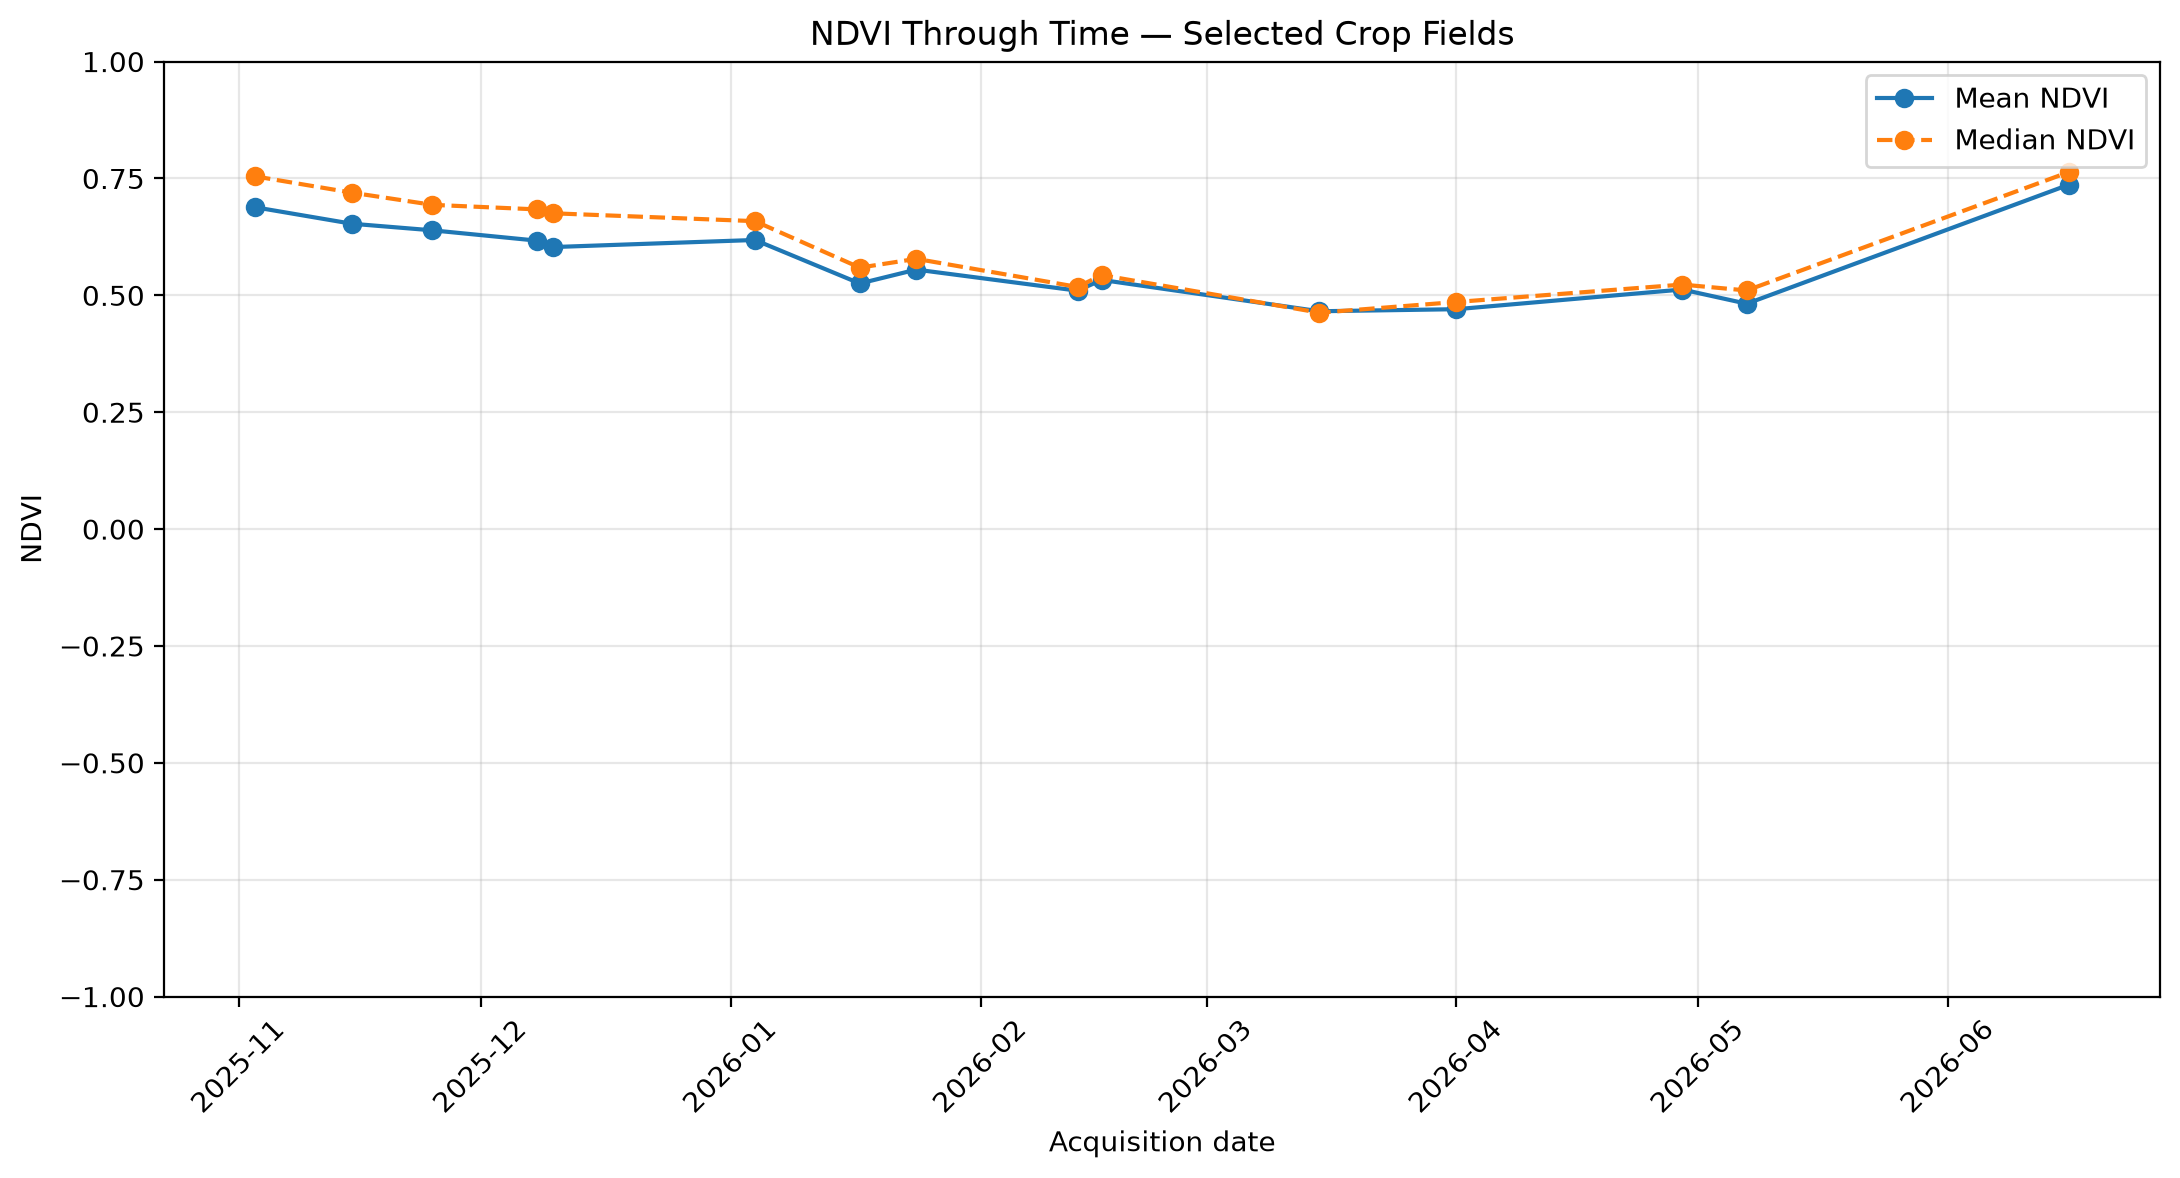
\includegraphics[
	width=0.95\linewidth
	]{../figures/stage5_figure_67.png}
	
	\caption{
		Temporal evolution of mean
		and median NDVI across the
		selected agricultural region
		for the 15 accepted Sentinel-2
		acquisitions from November
		2025 to June 2026.
	}
	
	\label{fig:ndvi_temporal_variability}
\end{figure}

The mean and median series
exhibited broadly similar
temporal patterns.

However, their differences
at individual acquisition dates
indicate that the distributions
were not necessarily symmetric
throughout the observation period.

The regional statistics describe
changes in satellite-derived
vegetation-index values and
do not independently establish
the agricultural or environmental
processes responsible for them.


\subsection{NDVI Distribution and Spatial Variability}
\label{subsec:ndvi_distribution_spatial}

Pixel-level NDVI distributions
were examined to characterize
variability within the selected
agricultural region.

Boxplots for the 15 accepted
acquisitions are presented in
\Cref{fig:ndvi_boxplots}.

\begin{figure}[htbp]
	\centering
	
	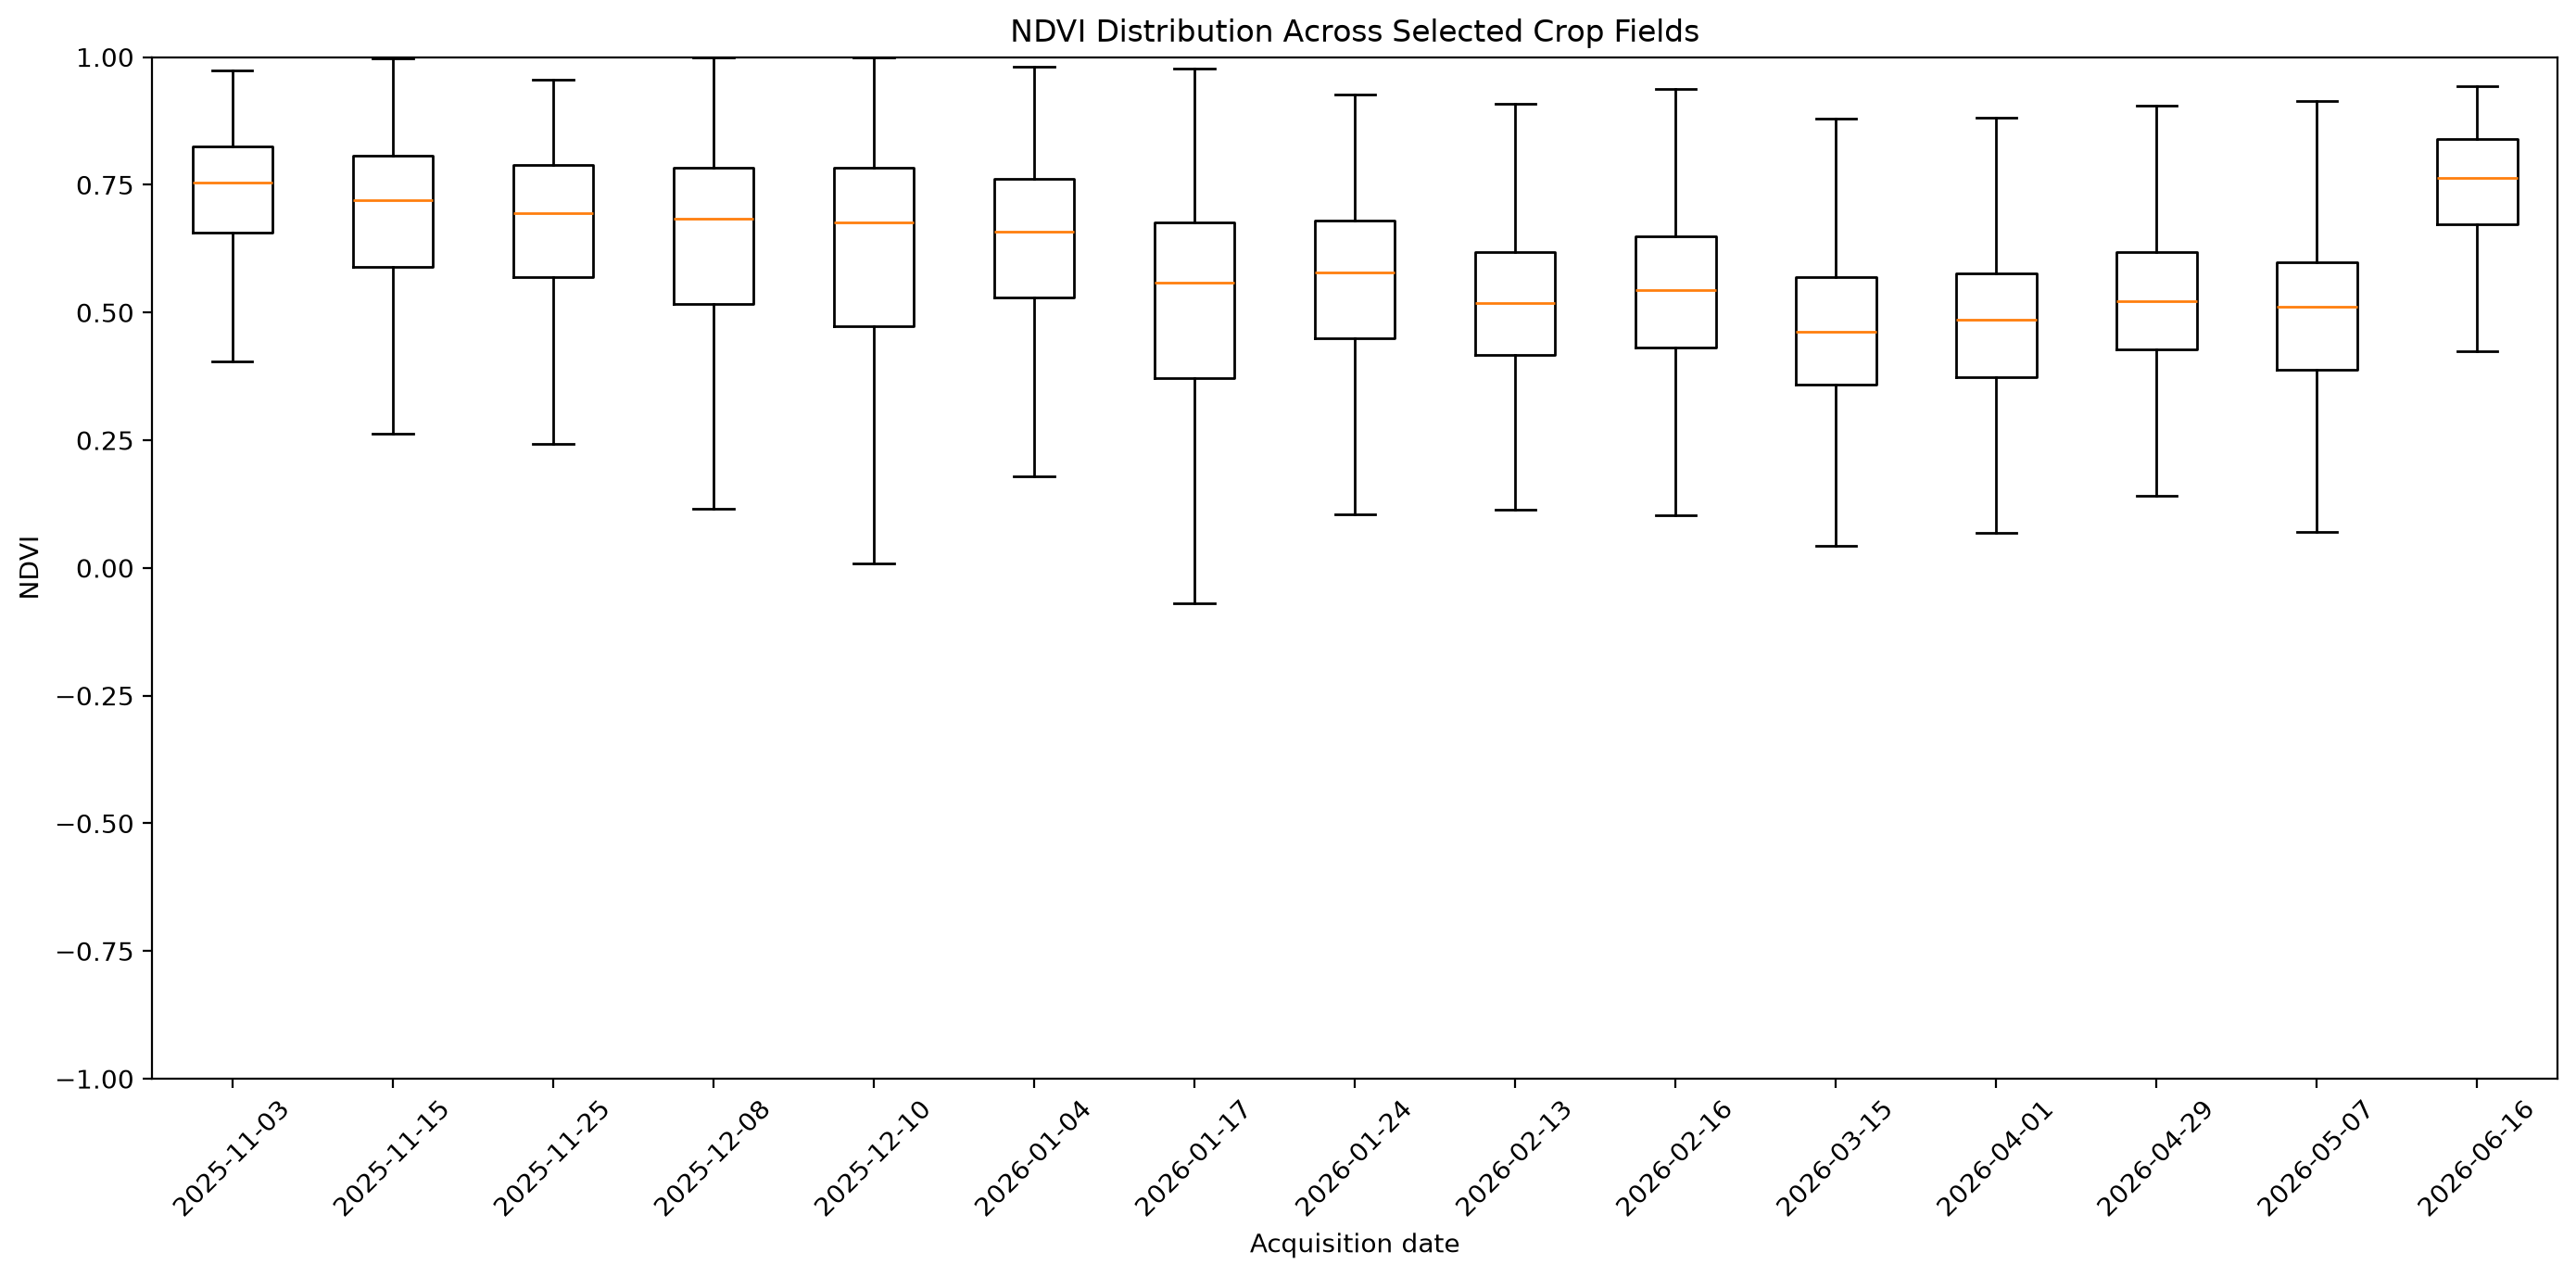
\includegraphics[
	width=0.95\linewidth
	]{../figures/stage5_figure_70.png}
	
	\caption{
		Pixel-level NDVI distributions
		across the 15 accepted
		Sentinel-2 acquisitions,
		represented by boxplots.
	}
	
	\label{fig:ndvi_boxplots}
\end{figure}

The distributions showed changes
in median NDVI, interquartile
range, and overall dispersion
across acquisition dates.

A general shift toward lower
NDVI values was observed between
November 2025 and March 2026,
consistent with the regional
mean and median time series.

To examine differences in
distribution shape, four
representative acquisitions
were selected:

8 December 2025,
16 February 2026,
29 April 2026, and
16 June 2026.

Their NDVI density distributions
are shown in
\Cref{fig:ndvi_density}.

\begin{figure}[htbp]
	\centering
	
	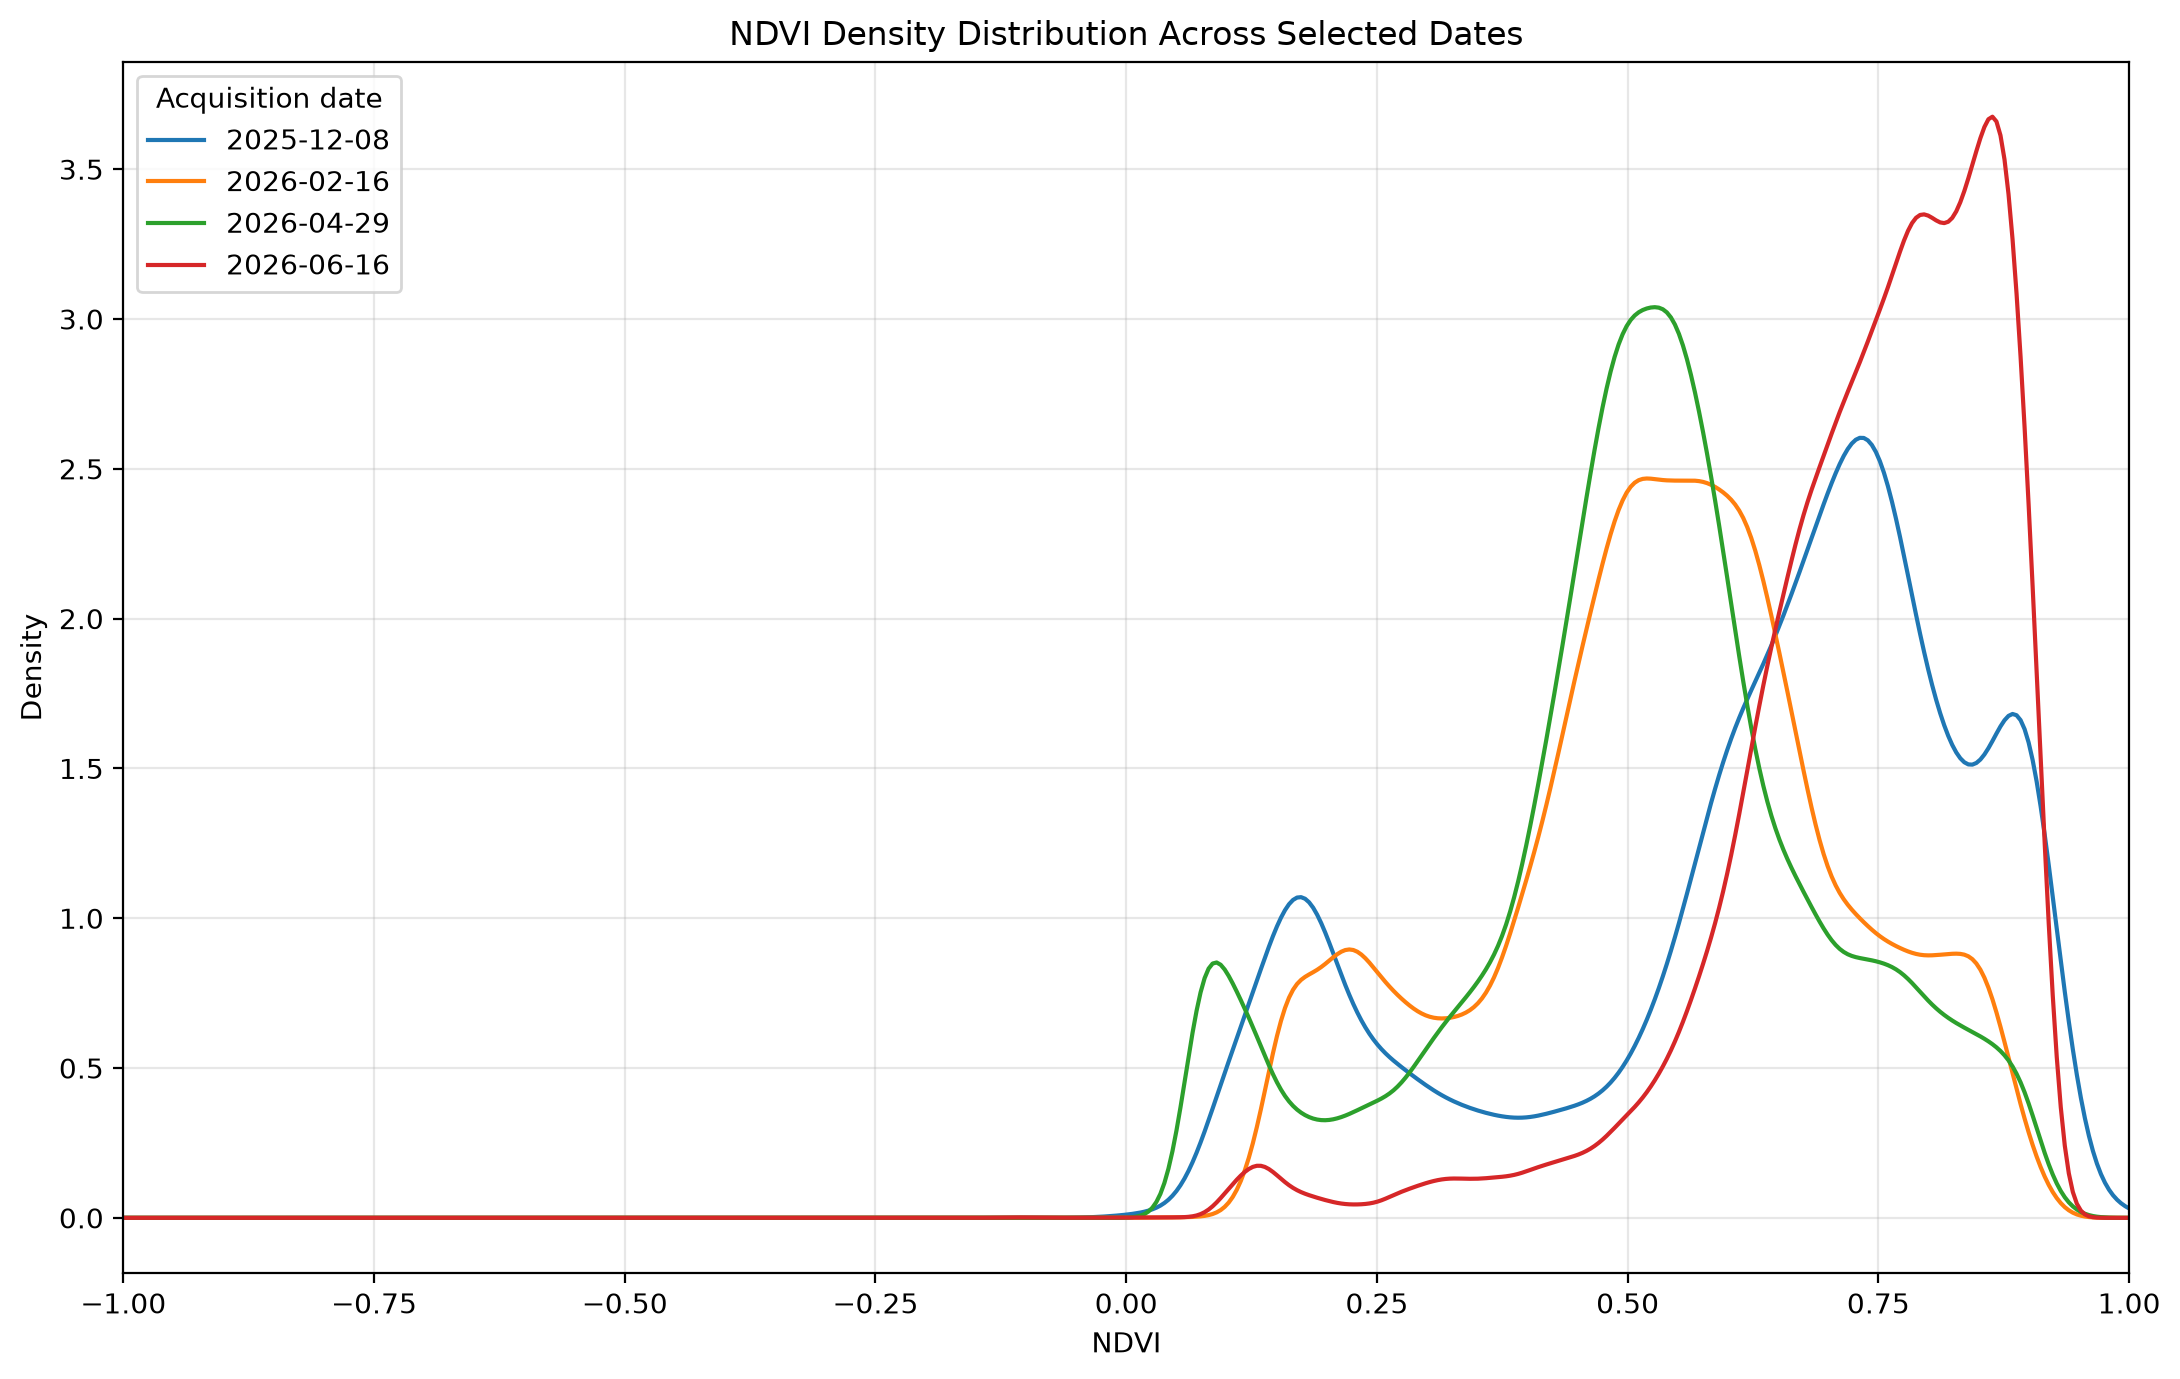
\includegraphics[
	width=0.95\linewidth
	]{../figures/stage5_figure_74.png}
	
	\caption{
		Pixel-level NDVI density
		distributions for four
		representative acquisitions:
		8 December 2025,
		16 February 2026,
		29 April 2026, and
		16 June 2026.
	}
	
	\label{fig:ndvi_density}
\end{figure}

The density curves showed
differences in the relative
frequency of low, intermediate,
and high NDVI values.

These changes indicate that
temporal variability was not
limited to shifts in the
regional mean.

The spatial distribution of
NDVI was also examined for
the same four acquisitions,
as shown in
\Cref{fig:ndvi_spatial_maps}.

\begin{figure}[htbp]
	\centering
	
	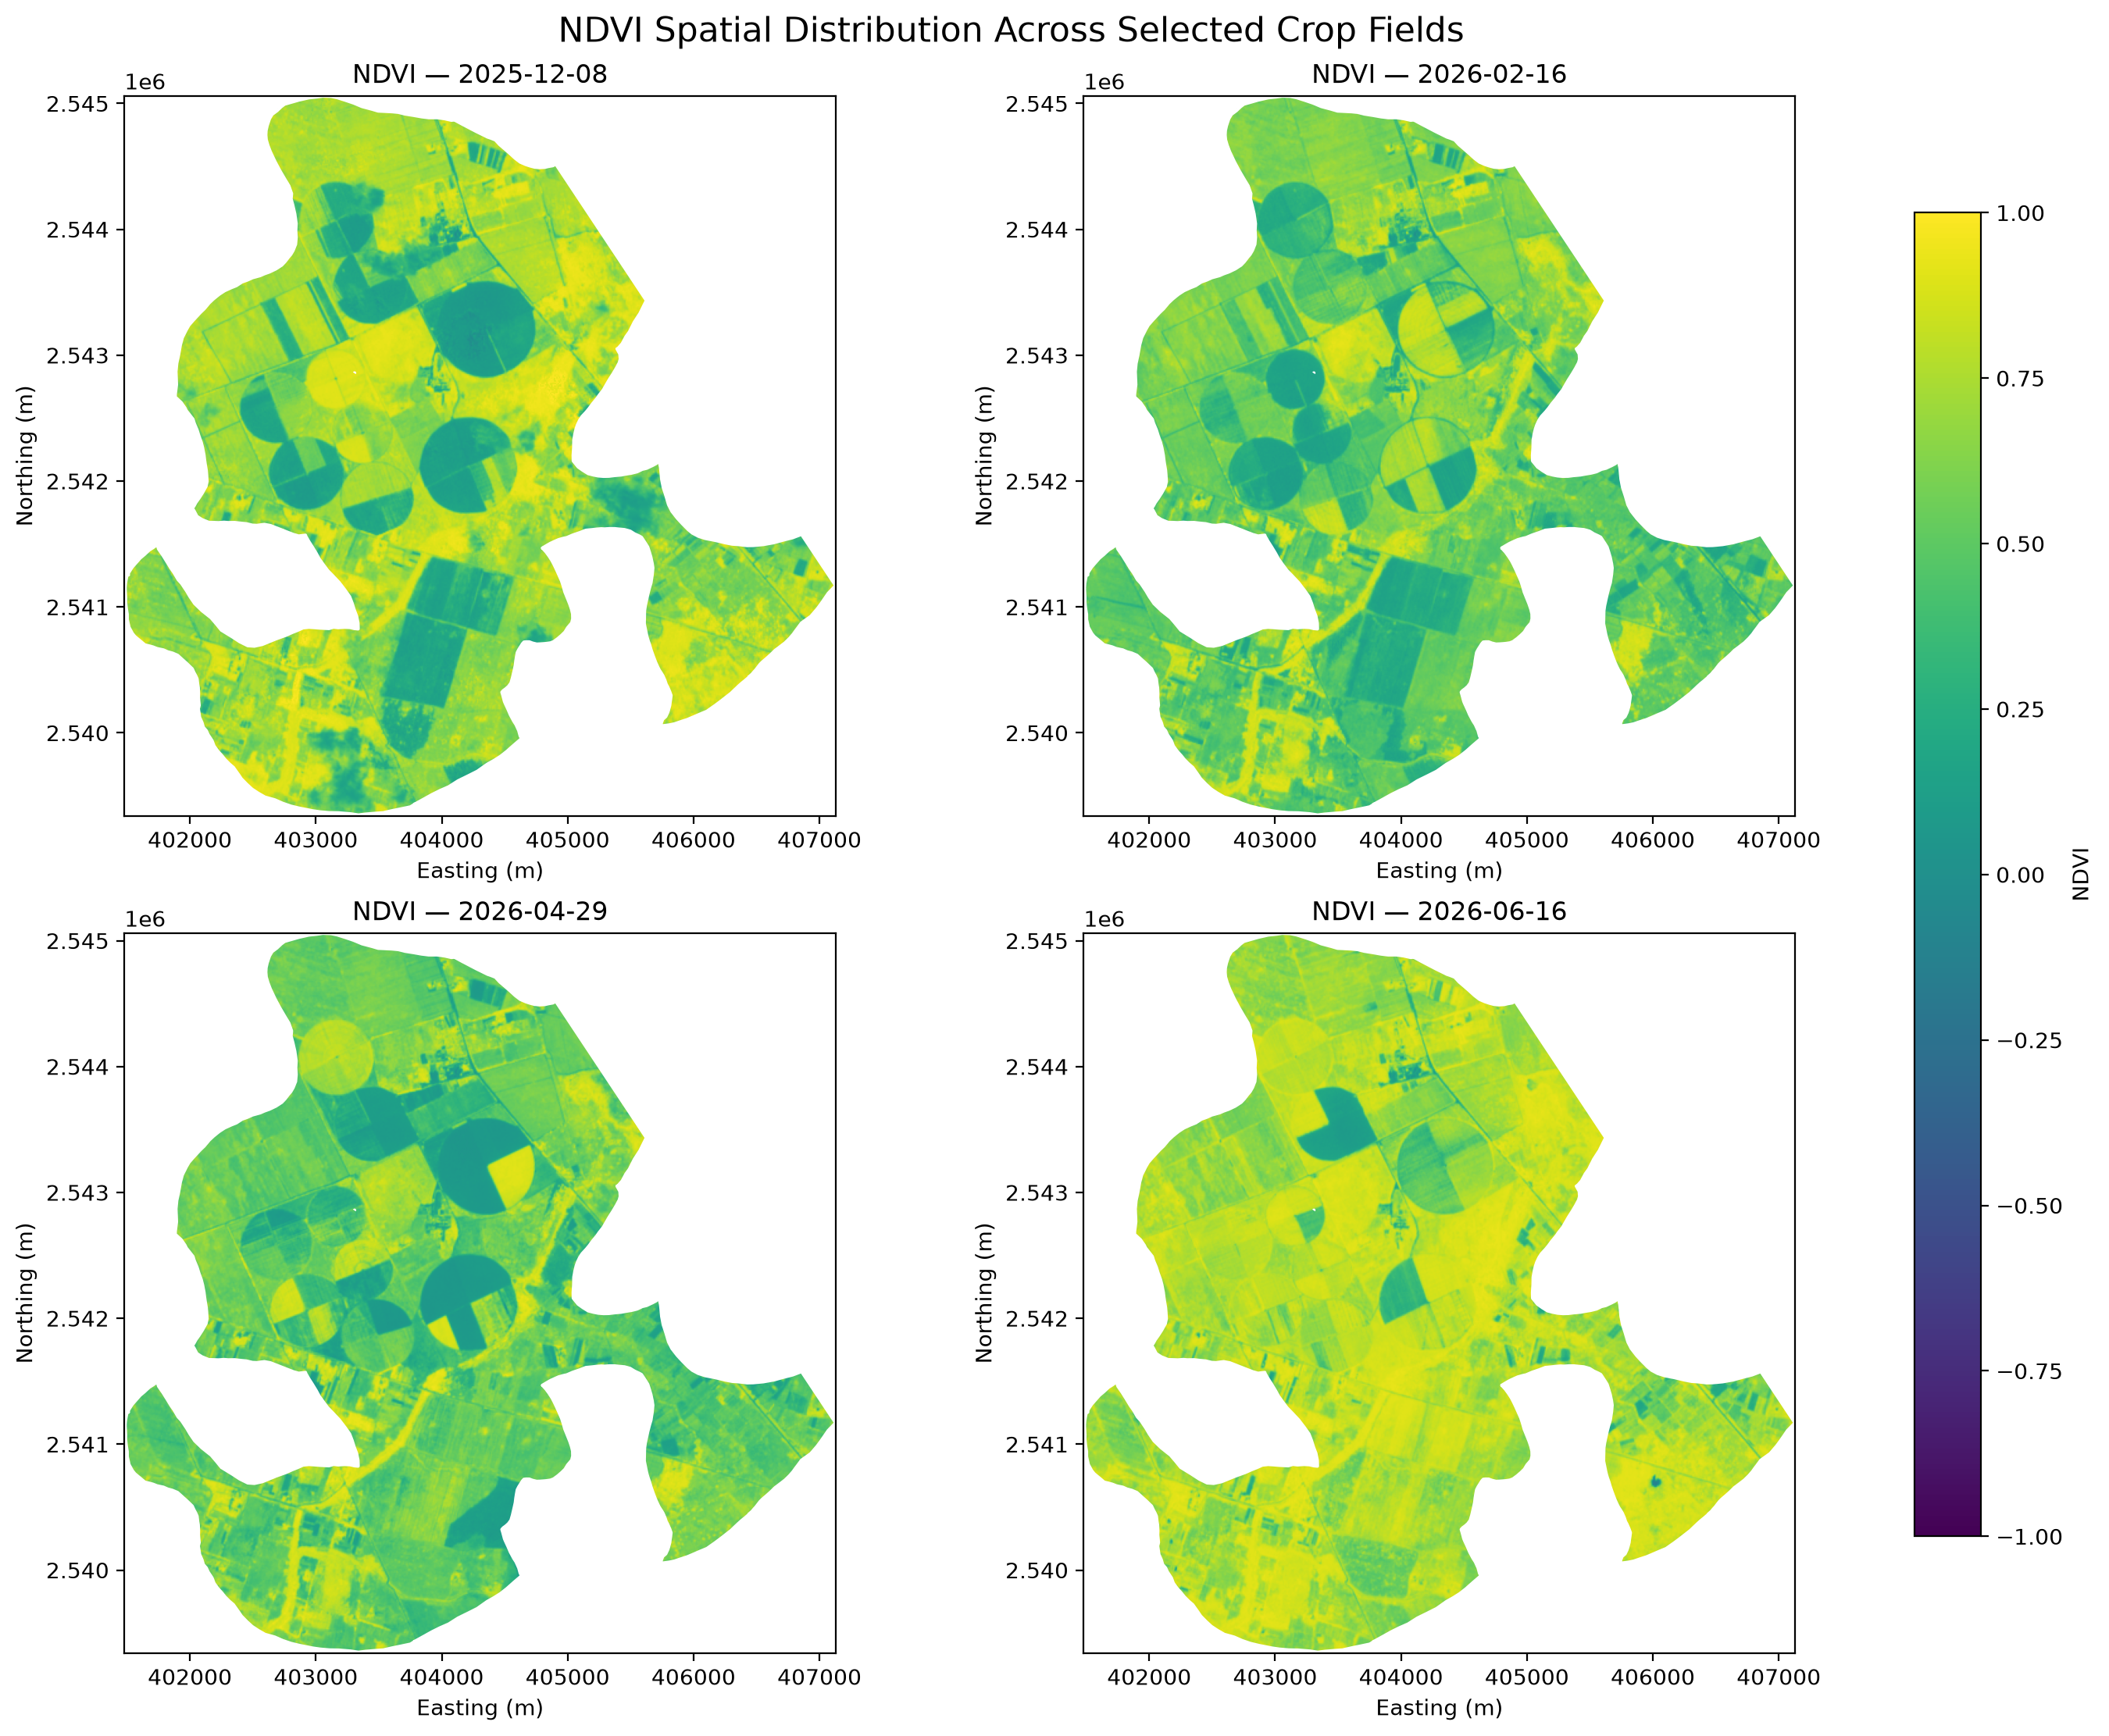
\includegraphics[
	width=\linewidth
	]{../figures/stage5_figure_76.png}
	
	\caption{
		Spatial distribution of
		NDVI within the selected
		agricultural region on
		8 December 2025,
		16 February 2026,
		29 April 2026, and
		16 June 2026.
		All panels use the same
		NDVI scale.
	}
	
	\label{fig:ndvi_spatial_maps}
\end{figure}

The maps revealed geographic
differences in NDVI within
the agricultural region.

Relatively high and low
vegetation-index values were
not distributed uniformly
across the selected polygons.

The June observation exhibited
higher regional NDVI values
than those recorded during
March and April.

However, these regional
distributions include multiple
agricultural and vegetation
conditions and cannot be
interpreted as observations
of potato cultivation alone.


\subsection{Field-Level NDVI Analysis of Selected Potato Fields}
\label{subsec:potato_field_analysis}

A complementary field-level
analysis examined three
locally verified potato fields
within the agricultural region.

The fields were represented
by circular sampling polygons
digitized in QGIS.

Their locations and the
sampling configuration are
illustrated in
\Cref{fig:potato_field_selection}.

\begin{figure}[htbp]
	\centering
	
	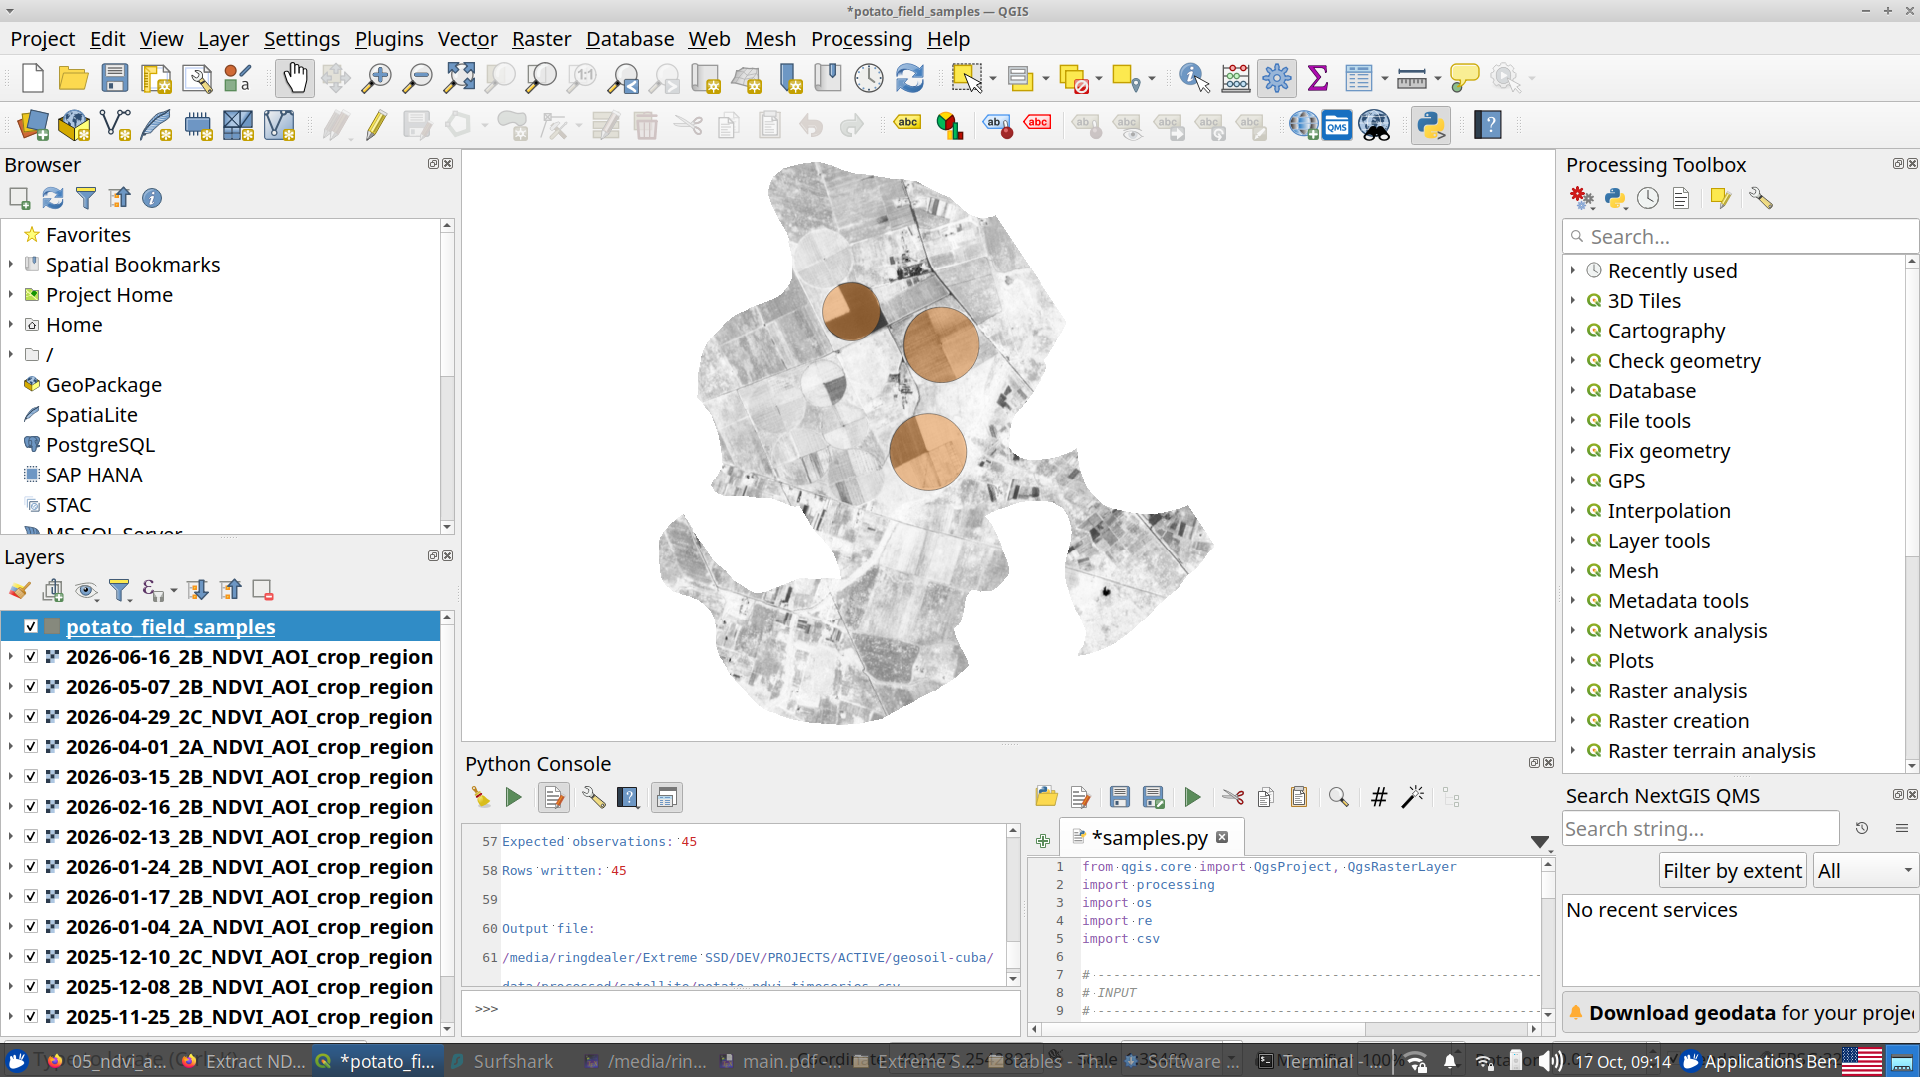
\includegraphics[
	width=\linewidth
	]{../figures/potato_samples.png}
	
	\caption{
		Three locally verified
		potato-field sampling areas
		digitized in QGIS and
		displayed over the
		agricultural-region
		NDVI raster.
	}
	
	\label{fig:potato_field_selection}
\end{figure}

NDVI observations were extracted
for each sampling polygon across
the 15 accepted acquisition dates,
yielding 45 field-date observations.

The number of valid pixels
differed among the sampling
polygons but remained constant
across the acquisition dates
for each field.

Field 1 contained 4,603 valid
pixels, Field 2 contained
4,785 pixels, and Field 3
contained 2,710 pixels.

The temporal evolution of
mean NDVI for the three fields
is presented in
\Cref{fig:potato_field_timeseries}.

\begin{figure}[htbp]
	\centering
	
	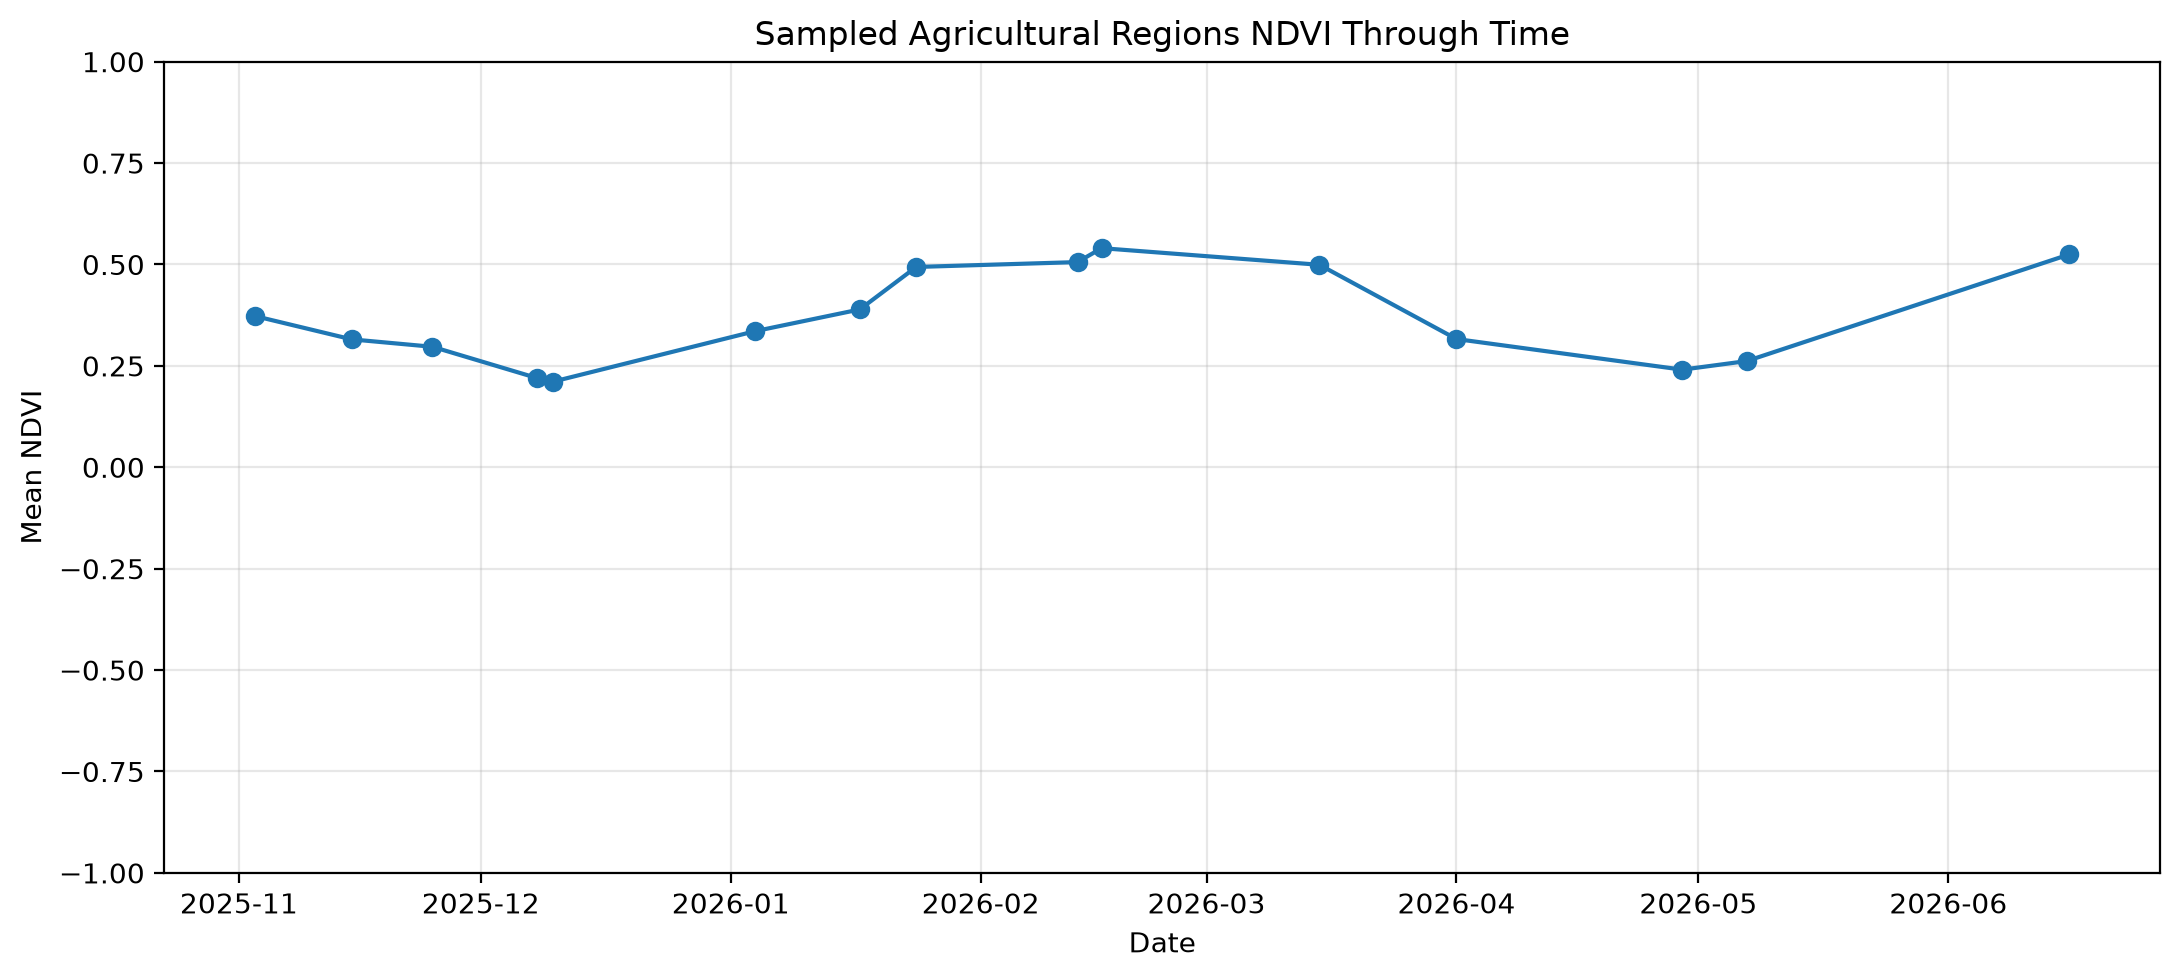
\includegraphics[
	width=0.95\linewidth
	]{../figures/stage5_figure_84.png}
	
	\caption{
		Temporal evolution of
		mean NDVI across the
		three selected potato-field
		sampling areas from
		November 2025 to June 2026.
	}
	
	\label{fig:potato_field_timeseries}
\end{figure}

The three sampled areas exhibited
different temporal NDVI patterns.

Field 1 reached its highest
mean NDVI of approximately
0.744 on 15 March 2026.

Field 2 reached its highest
mean NDVI of approximately
0.690 on 16 June 2026.

Field 3 reached its highest
mean NDVI of approximately
0.573 on 24 January 2026,
followed by a substantial
decline in subsequent
observations.

The maximum observed mean NDVI
values and their corresponding
dates are summarized in
\Cref{tab:potato_field_maxima}.

\begin{table}[htbp]
	\centering
	
	\caption{
		Maximum observed mean NDVI
		for the three selected
		potato-field sampling areas.
	}
	
	\label{tab:potato_field_maxima}
	
	\begin{tabular}{lcc}
		\hline
		
		\textbf{Field} &
		\textbf{Maximum mean NDVI} &
		\textbf{Acquisition date} \\
		
		\hline
		
		Field 1 & 0.744 & 15 March 2026 \\
		Field 2 & 0.690 & 16 June 2026 \\
		Field 3 & 0.573 & 24 January 2026 \\
		
		\hline
	\end{tabular}
\end{table}

The different dates of
maximum mean NDVI indicate
that the sampled fields
did not follow identical
vegetation-index trajectories.

Pixel-level NDVI distributions
were also examined using
boxplots, as presented in
\Cref{fig:potato_field_boxplots}.

\begin{figure}[htbp]
	\centering
	
	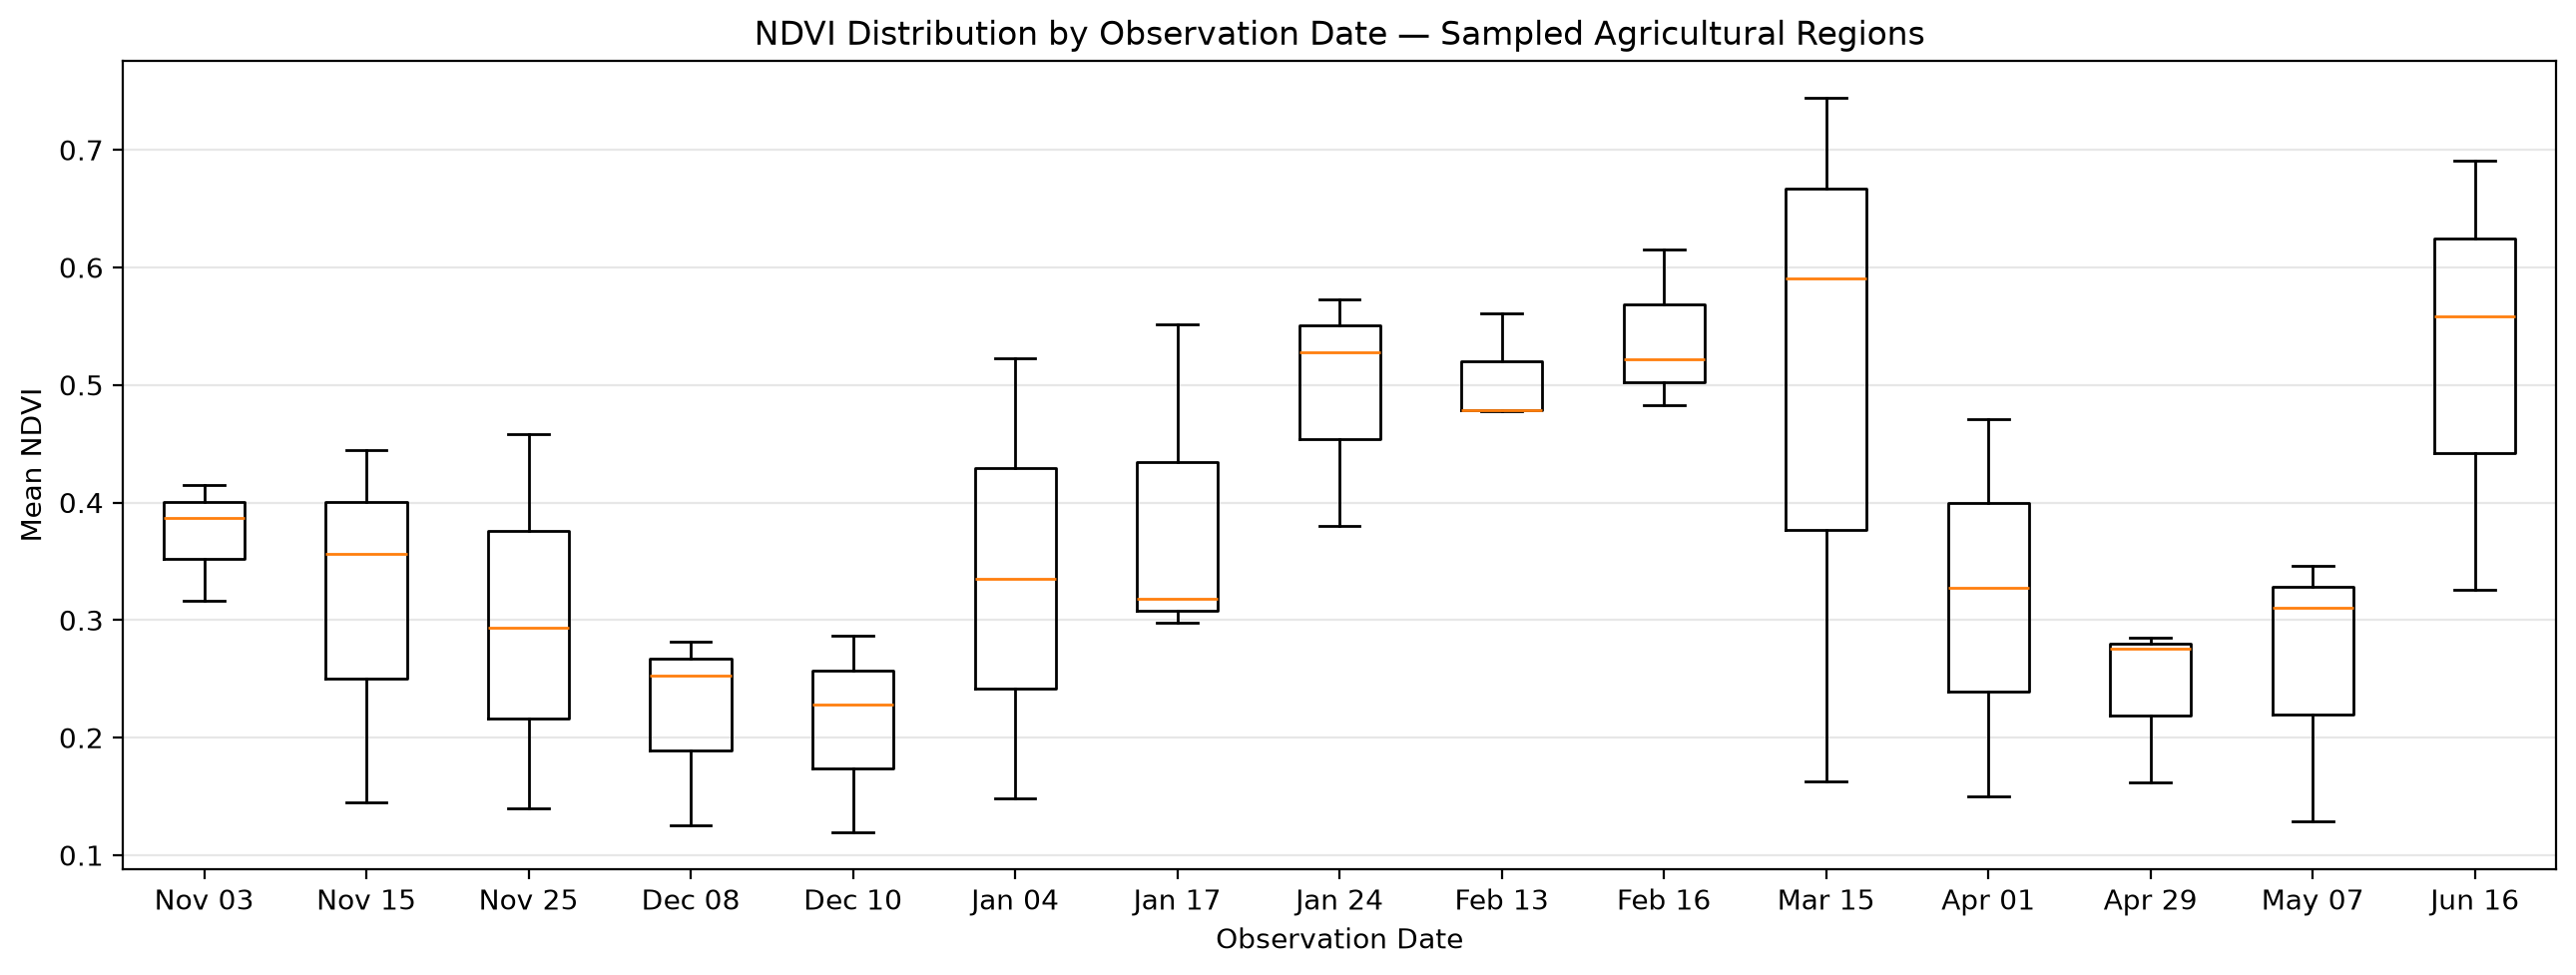
\includegraphics[
	width=0.95\linewidth
	]{../figures/stage5_figure_86}
	
	\caption{
		Distribution of NDVI
		observations across the
		three selected potato-field
		sampling areas and
		acquisition dates.
	}
	
	\label{fig:potato_field_boxplots}
\end{figure}

The field-level results
demonstrate temporal variability
within the selected agricultural
sampling areas that is not
fully represented by the
regional mean NDVI series.

The observed differences
provide a basis for further
investigation of agricultural
conditions but do not
independently identify
crop-development stages,
harvesting dates, or
management practices.
	\section{Discussion and Limitations}
\label{sec:discussion}

\subsection{Spatial Data Integration and Map Completeness}

The results demonstrate the importance of evaluating
geometric consistency and spatial coverage before using
historical soil cartography in contemporary GIS analysis.
Within the 178.47~km$^2$ Area of Interest (AOI), the
soil polygons covered approximately 162.852~km$^2$,
measured as their geometric union in EPSG:3795.
Of the 15.62~km$^2$ not covered by soil polygons,
approximately 11.42~km$^2$ corresponded to mapped
water surfaces, leaving 4.20~km$^2$ of non-water gaps.

Distinguishing water surfaces from unresolved gaps
prevents the absence of terrestrial soil polygons
over the reservoir from being incorrectly interpreted
as a soil-mapping defect. The remaining gaps require
examination against the original cartography and
other authoritative spatial sources before they
can be classified or filled.

Topology checks identified 90 polygon pairs with
positive-area intersections. Their cumulative
pairwise overlap area was approximately
0.054919~km$^2$. Although small relative to the
mapped extent, these overlaps can introduce
duplicate area contributions in spatial summaries
and overlay operations.

The original geometries were preserved to maintain
data provenance. Consequently, the processed dataset
should not be described as fully topologically
corrected. Area statistics based on sums of individual
polygons must be distinguished from statistics based
on their geometric union. Furthermore, cumulative
pairwise overlap areas do not necessarily equal the
geographic area affected by overlaps when three or
more polygons intersect.

Area calculations also varied slightly with the
coordinate reference system (CRS). In EPSG:3795,
the sum of individual polygon areas was
162.907~km$^2$, while their geometric union covered
162.852~km$^2$. After reprojection to EPSG:32617,
the corresponding values were 162.820~km$^2$
and 162.766~km$^2$, respectively. The union area
decreased by approximately 0.086~km$^2$
(0.053\%) after reprojection. In both CRSs,
the difference between the polygon-area sum and
the geometric union remained approximately
0.055~km$^2$, consistent with the contribution
of overlapping polygons to the summed area.
These results emphasize the need to specify the
CRS and area-calculation method when reporting
spatial coverage.

The integration of soil and vegetation polygons
provides a common spatial framework for examining
mapped attributes. Nevertheless, spatial coincidence
does not establish that a soil class determines
the observed vegetation condition. The source
layers may differ in production date, mapping
purpose, classification criteria, and positional
accuracy. These differences limit the interpretation
of direct spatial comparisons.

An additional area-accounting issue concerns the
vegetation dataset. The four reported vegetation
class areas sum to approximately 178.47~km$^2$,
whereas the stated vegetation coverage is
161.93~km$^2$. Their mutual exclusivity, possible
overlaps, and the corresponding area-calculation
procedures must therefore be verified before the
categories can be interpreted as an additive
partition of the AOI.


\subsection{Interpretation of Regional NDVI Dynamics}

The 15 retained Sentinel-2 observations show
substantial temporal variation within the selected
16.22~km$^2$ agricultural region.

Mean NDVI declined from approximately 0.688
on 3 November 2025 to 0.466 on 15 March 2026,
then varied during April and May before reaching
approximately 0.737 on 16 June 2026.

The boxplots, density curves, and spatial maps
indicate that these changes involved both
regional central tendency and the spatial
distribution of NDVI values.

These observations are consistent with changes
in vegetation conditions across an actively
managed agricultural landscape, but they do
not independently identify their causes.

The selected region contains multiple agricultural
polygons rather than an independently verified
single-crop planting area. Consequently, its
aggregate trajectory cannot be interpreted as
a potato growth curve.

Changes in crop composition, planting and
harvesting schedules, vegetation regrowth,
weeds, moisture conditions, and residual
image contamination could contribute to
the observed signal.

In particular, the June increase cannot be
attributed to a specific crop or management
practice without additional field evidence.

The regional analysis is descriptive rather
than causal. The association of the selected
polygons with mapped Ferrallitic soil units
provides geographic context, but the analysis
does not control for irrigation, agricultural
management, crop identity, or other potential
confounding factors.

The results therefore do not support claims
that one mapped soil class produced higher
NDVI or better crop performance than another.


\subsection{Field-Level Observations and Agricultural Context}

The three locally verified potato fields
provide a more specific spatial reference
than the broader agricultural region.

Their NDVI trajectories were not uniform.
Among the retained observations, the highest
mean NDVI occurred on 15 March 2026 in Field~1,
on 16 June 2026 in Field~2, and on
24 January 2026 in Field~3.

These differences illustrate why an aggregate
regional NDVI curve should not be interpreted
as representative of every individual field.

However, the dates of the highest observed
mean NDVI values do not necessarily represent
the actual seasonal vegetation maxima.
Unobserved peaks may have occurred between
the available satellite acquisitions.

Local verification supports the identification
of the sampling locations as potato fields,
but it does not establish that potatoes
occupied each sampled polygon continuously
throughout the November 2025--June 2026
observation period.

In particular, post-harvest NDVI may reflect
subsequent crops, vegetation regrowth, weeds,
or other vegetation rather than the original
potato crop.

The circular sampling polygons are
approximations rather than surveyed field
boundaries. Their geometry and placement
may therefore influence the extracted NDVI
statistics, particularly where sampling
areas intersect heterogeneous vegetation
or field boundaries.

Field-specific planting dates, harvesting
records, accurate field boundaries, and
repeated ground observations would be
needed to assign crop-development stages
and interpret field-level differences
with greater confidence.


\subsection{Remote-Sensing and Reproducibility Limitations}

The regional quality filter retained
acquisitions with less than 10\% cloud
coverage according to the selected SCL
cloud classes.

This acquisition-level threshold reduces
potential contamination but does not
guarantee that every pixel used for NDVI
statistics is free from clouds, cirrus,
haze, or shadows.

Cloud shadows were evaluated separately,
and numerical NDVI validity alone does
not constitute a cloud mask.

Future analyses should implement and
document explicit pixel-level quality
masks, including cloud shadows and
other unsuitable SCL classes, and report
the number and proportion of usable
pixels for each acquisition.

The temporal sample is also irregular.
Fifteen retained dates span November
2025 through June 2026, with unequal
intervals between observations.

These data support comparisons among
the retained acquisition dates but do
not provide a continuously observed
vegetation-development curve.

Short-lived changes and seasonal
maxima may have occurred between
acquisitions. Furthermore, the nearly
constant number of numerically valid
pixels does not independently establish
equivalent atmospheric quality across
the observations.

Radiometric preprocessing used a
quantification factor of 10,000 and
an additive offset of $-1000$ for
both spectral bands, based on inspection
of 111 available product metadata files.

These parameters were also applied
to some images without individually
available XML metadata.

Although this assumption was documented,
product-specific verification remains
necessary to establish the consistency
of radiometric preprocessing across
the full time series.

Unlike a common multiplicative factor,
an additive radiometric offset does
not cancel during NDVI calculation.
Consequently, incorrect offset
parameters may affect the resulting
vegetation-index values.

Additional sources of uncertainty
include the 10~m spatial resolution
of the spectral bands, the 20~m
resolution of the SCL, resampling
choices, and potential positional
differences between historical
vector boundaries and satellite
imagery.

Overall, the principal contribution
of GeoSoil-Cuba is a documented and
reproducible workflow for integrating
historical soil cartography, existing
land-cover information, and
satellite-derived vegetation indices.

The results support spatial
data-quality assessment and
exploratory vegetation monitoring,
but they do not independently
validate soil properties, crop
yield, or causal relationships
between soil classes and
agricultural performance.

The principal priorities for
further development are targeted
topology review, harmonized area
accounting, product-specific
radiometric verification,
explicit pixel-level quality
masking, and field observations
aligned with satellite
acquisition dates.
	\section{Conclusions and Future Work}
\label{sec:conclusions}

GeoSoil-Cuba demonstrates an open-source geospatial
workflow for preparing historical soil cartography,
integrating soil and vegetation attributes, and
examining Sentinel-2 NDVI observations within an
agricultural landscape in Jaruco, Mayabeque, Cuba.
The analysis combines vector-data validation,
coordinate reference system harmonization,
spatial overlay, satellite-image processing,
and temporal vegetation-index analysis within
a documented GIS and Python environment.

Within the 178.47~km$^2$ study area, the soil
coverage assessment reported approximately
162.85~km$^2$ of mapped soil units. Accounting
for mapped water surfaces reduced the remaining
non-water soil-data gaps to approximately
4.20~km$^2$, equivalent to 2.35\% of the AOI.
Topology assessment identified 90 overlapping
polygon pairs with a cumulative pairwise overlap
area of approximately 0.054919~km$^2$.
These findings highlight the importance of
evaluating spatial coverage, geometric consistency,
and area-accounting procedures before interpreting
historical soil-map information.

Satellite processing produced 32 regional NDVI
rasters, of which 15 acquisitions satisfied
the regional cloud-coverage criterion.
Within the selected 16.22~km$^2$ agricultural
region, mean NDVI declined between November 2025
and March 2026, followed by fluctuations and
an increase by June 2026. A complementary
analysis of three locally verified potato fields
revealed different temporal NDVI trajectories,
illustrating the importance of distinguishing
field-level observations from regional aggregates.

The findings characterize spatial and temporal
patterns in the available datasets but do not
establish crop phenological stages, agricultural
productivity, or causal relationships between
soil classes and vegetation conditions.
Interpretation remains constrained by uncertainties
in historical mapping, unresolved topology and
area-accounting discrepancies, irregular satellite
sampling, residual cloud contamination, and
incomplete field and radiometric metadata
verification.

Future development should prioritize reconciling
soil and vegetation area calculations, reviewing
overlapping soil polygons and remaining non-water
gaps, verifying radiometric parameters for
individual satellite products, and implementing
explicit pixel-level cloud and shadow masking.
Additional improvements should include accurate
agricultural field boundaries, planting and
harvesting records, and ground observations
corresponding to satellite acquisition dates.
These developments would provide a stronger
basis for evaluating vegetation variability
across mapped soil units and agricultural
management conditions.

The resulting framework provides a foundation
for further geospatial research and potential
application in other regions where historical
soil cartography, ancillary land-cover data,
and contemporary satellite observations must
be integrated while preserving data provenance
and documenting uncertainty.
	
	\section*{Acknowledgments}
	
	The author acknowledges the Faculty of Geography,
	University of Havana, Cuba (Facultad de Geografía,
	Universidad de La Habana), for providing the soil,
	water-body, and vegetation-cover datasets used in
	this study and authorizing their use for research,
	analysis, and public redistribution.
	
	% --------------------------------------------------
	% AI Assistance and Author Responsibility
	% --------------------------------------------------
	
	\section*{AI Assistance and Author Responsibility}
\label{sec:author-ai}

Generative AI tools were used to assist with the
organization, drafting, and revision of this article.
The author is responsible for the research workflow,
the interpretation of the results, and the final
content of the manuscript. The reported methods,
quantitative results, and references were reviewed
against the available data and source materials.
	
	
	
	% --------------------------------------------------
	% References
	% --------------------------------------------------
	\printbibliography
	
\end{document}